\documentclass[twoside]{book}

% Packages required by doxygen
\usepackage{fixltx2e}
\usepackage{calc}
\usepackage{doxygen}
\usepackage[export]{adjustbox} % also loads graphicx
\usepackage{graphicx}
\usepackage[utf8]{inputenc}
\usepackage{makeidx}
\usepackage{multicol}
\usepackage{multirow}
\PassOptionsToPackage{warn}{textcomp}
\usepackage{textcomp}
\usepackage[nointegrals]{wasysym}
\usepackage[table]{xcolor}

% Font selection
\usepackage[T1]{fontenc}
\usepackage[scaled=.90]{helvet}
\usepackage{courier}
\usepackage{amssymb}
\usepackage{sectsty}
\renewcommand{\familydefault}{\sfdefault}
\allsectionsfont{%
  \fontseries{bc}\selectfont%
  \color{darkgray}%
}
\renewcommand{\DoxyLabelFont}{%
  \fontseries{bc}\selectfont%
  \color{darkgray}%
}
\newcommand{\+}{\discretionary{\mbox{\scriptsize$\hookleftarrow$}}{}{}}

% Page & text layout
\usepackage{geometry}
\geometry{%
  a4paper,%
  top=2.5cm,%
  bottom=2.5cm,%
  left=2.5cm,%
  right=2.5cm%
}
\tolerance=750
\hfuzz=15pt
\hbadness=750
\setlength{\emergencystretch}{15pt}
\setlength{\parindent}{0cm}
\setlength{\parskip}{3ex plus 2ex minus 2ex}
\makeatletter
\renewcommand{\paragraph}{%
  \@startsection{paragraph}{4}{0ex}{-1.0ex}{1.0ex}{%
    \normalfont\normalsize\bfseries\SS@parafont%
  }%
}
\renewcommand{\subparagraph}{%
  \@startsection{subparagraph}{5}{0ex}{-1.0ex}{1.0ex}{%
    \normalfont\normalsize\bfseries\SS@subparafont%
  }%
}
\makeatother

% Headers & footers
\usepackage{fancyhdr}
\pagestyle{fancyplain}
\fancyhead[LE]{\fancyplain{}{\bfseries\thepage}}
\fancyhead[CE]{\fancyplain{}{}}
\fancyhead[RE]{\fancyplain{}{\bfseries\leftmark}}
\fancyhead[LO]{\fancyplain{}{\bfseries\rightmark}}
\fancyhead[CO]{\fancyplain{}{}}
\fancyhead[RO]{\fancyplain{}{\bfseries\thepage}}
\fancyfoot[LE]{\fancyplain{}{}}
\fancyfoot[CE]{\fancyplain{}{}}
\fancyfoot[RE]{\fancyplain{}{\bfseries\scriptsize Generated by Doxygen }}
\fancyfoot[LO]{\fancyplain{}{\bfseries\scriptsize Generated by Doxygen }}
\fancyfoot[CO]{\fancyplain{}{}}
\fancyfoot[RO]{\fancyplain{}{}}
\renewcommand{\footrulewidth}{0.4pt}
\renewcommand{\chaptermark}[1]{%
  \markboth{#1}{}%
}
\renewcommand{\sectionmark}[1]{%
  \markright{\thesection\ #1}%
}

% Indices & bibliography
\usepackage{natbib}
\usepackage[titles]{tocloft}
\setcounter{tocdepth}{3}
\setcounter{secnumdepth}{5}
\makeindex

% Hyperlinks (required, but should be loaded last)
\usepackage{ifpdf}
\ifpdf
  \usepackage[pdftex,pagebackref=true]{hyperref}
\else
  \usepackage[ps2pdf,pagebackref=true]{hyperref}
\fi
\hypersetup{%
  colorlinks=true,%
  linkcolor=blue,%
  citecolor=blue,%
  unicode%
}

% Custom commands
\newcommand{\clearemptydoublepage}{%
  \newpage{\pagestyle{empty}\cleardoublepage}%
}

\usepackage{caption}
\captionsetup{labelsep=space,justification=centering,font={bf},singlelinecheck=off,skip=4pt,position=top}

%===== C O N T E N T S =====

\begin{document}

% Titlepage & ToC
\hypersetup{pageanchor=false,
             bookmarksnumbered=true,
             pdfencoding=unicode
            }
\pagenumbering{roman}
\begin{titlepage}
\vspace*{7cm}
\begin{center}%
{\Large Shoot \textquotesingle{}Em All }\\
\vspace*{1cm}
{\large Generated by Doxygen 1.8.11}\\
\end{center}
\end{titlepage}
\clearemptydoublepage
\tableofcontents
\clearemptydoublepage
\pagenumbering{arabic}
\hypersetup{pageanchor=true}

%--- Begin generated contents ---
\chapter{Shoot \textquotesingle{}Em All}
\label{index}\hypertarget{index}{}\subsection*{Authors}


\begin{DoxyItemize}
\item Kasper De Volder
\item Brian Segers
\item Vladimir Poliakov
\end{DoxyItemize}

\subsection*{Documentation}

Doxygen generated documentation is available in docs/html/index.\+html

\subsection*{Game description}

The point of the game is to defeat all enemies and stay alive. Protagonist can only move while his energy level is higher than zero. Protagonist will not move if the target point is further than he can afford with energy that he has at the moment. Every time protagonist moves according amount of energy is being spent. Every time protagonist interact with an object, e.\+g. picks up a health pack or attack the enemy, the energy level is restored.

The hero can die because of two reasons\+:
\begin{DoxyItemize}
\item The enemy that hero has attacked is stronger than the hero\textquotesingle{}s health level
\item The hero has been poisoned with a poison level bigger than hero\textquotesingle{}s health level. In that case the protagonist still has one move to pick a health pack before he will die.
\end{DoxyItemize}

Before starting the game, player should pick the level, number of enemies and health packs in the world and a level of optimization for the model\textquotesingle{}s controller\+:



Afterwards the main window will appear allowing player to move across the world and beat enemies\+:



Player can switch between graphical and terminal view at any moment by clicking {\ttfamily Switch view} button. Speed of animation can also be changed using {\ttfamily Set animation speed} slider. Player can change or restart the world any time by clicking {\ttfamily World-\/$>$Load world..}

\subsection*{Project description}

This project is an implementation of Media Processing course\textquotesingle{}s final task. The purpose is to create a game in which the player can mode across labyrinth and defeat enemies. The game should be implemented with two views\+: graphical and terminal-\/like.

In graphical view, the player can move with keyboard or mouse. Protagonist is displayed as blue circle, enemies are the red circles, poison area of the enemy is displayed as yellow circle, health packs are the green circles.

Protagonist path finding should be performed in shortest time possible. For that purpose some path finding algorithm should be introduced. Since different algorithms can be used/implemented, application should be able to use any of them, which means that a unified interface for path finding class should be implemented.

\subsection*{Main class diagram\+:}

Following diagram represents the model of the system divided into packages. Each package reprsesents separate module.



{\ttfamily libworld} is a third party library for generating the level and level objects\+: protagonist, health packs, enemies. {\ttfamily model} package represents the model component of the application. {\ttfamily terminalview} and {\ttfamily graphicsview} are view components of the system. {\ttfamily controller} package represents model controller component. Since different algorithms can be later implemented for path finding, abstract class {\ttfamily \hyperlink{classWorldAbstractController}{World\+Abstract\+Controller}} and factory class {\ttfamily \hyperlink{classWorldControllerFactory}{World\+Controller\+Factory}}are introduced.

\subsection*{Model package}

{\ttfamily model} package is the implementation of the model component of the application. {\ttfamily model} package class diagram is shown below\+:



{\ttfamily model} package includes {\ttfamily \hyperlink{classWorldModel}{World\+Model}} class. {\ttfamily \hyperlink{classWorldModel}{World\+Model}} stores information about the world and object that has been created (world tiles, health packs, enemies, protagonist, level image), as well as it provides interfaces to get information about the model to views. Model also owns its controller, which is used to perform protagonist movement. View can call protagonist movement by calling {\ttfamily \hyperlink{classWorldModel_ae02716d99230f6edb0f7caf5b469bc1c}{World\+Model\+::move()}} function.\+In that case, model will call appropriate controller function to find the shortest path to the target.

\subsection*{Controller package}

{\ttfamily controller} package includes abstract class {\ttfamily \hyperlink{classWorldAbstractController}{World\+Abstract\+Controller}}, one its successor {\ttfamily \hyperlink{classAStarController}{A\+Star\+Controller}}, and a factory class {\ttfamily \hyperlink{classWorldControllerFactory}{World\+Controller\+Factory}}. Following diagram visualizes their relations\+:



Static method {\ttfamily create\+Controller()} is used by \hyperlink{classWorldModel}{World\+Model} in order to create a controller of a certain type.\+In order to implement a new controller, it should be inherited from {\ttfamily Abstract\+Controller}, {\ttfamily find\+Path()} function should be implemented, and its type should be added to {\ttfamily Controller\+Type}enumeration. For demonstration purposes, only {\ttfamily \hyperlink{classAStarController}{A\+Star\+Controller}} is implemented.

\subsection*{Graphicsview package}

{\ttfamily graphicsview} package includes {\ttfamily \hyperlink{classWorldGraphicsView}{World\+Graphics\+View}} which is inherited from {\ttfamily Q\+Graphcis\+View}. Following diagram shows members and relations of {\ttfamily \hyperlink{classWorldGraphicsView}{World\+Graphics\+View}}\+:



{\ttfamily \hyperlink{classWorldGraphicsView}{World\+Graphics\+View}} class represents graphical view based on Qt\textquotesingle{}s Model-\/\+Scene-\/\+View technology. Once {\ttfamily set\+Model()} is called, {\ttfamily \hyperlink{classWorldGraphicsView}{World\+Graphics\+View}} draws level background and creates a graphical item {\ttfamily Q\+Graphics\+Ellipse} for each object with appropriate collor, as well as it connects each graphical item to its model object\textquotesingle{}s signals, so every change in the model is automatically impacts the view. Whenever model is reset or reloaded, old scene is being deleted along with its graphical items.

\subsection*{Terminalview package}

{\ttfamily terminalview} package represents the terminal view of the game. Following diagram shows members and relations of {\ttfamily \hyperlink{classWorldTerminalView}{World\+Terminal\+View}}\+:



It has a text field for output, edit line for command input and a button to execute the command(optionally can be done with {\ttfamily Enter}). When {\ttfamily execute\+Cmd()} is called, program reads the input and splits it into actual command and arguments. If no command was specified, help information is shown. Along with output for user commands, {\ttfamily \hyperlink{classWorldTerminalView}{World\+Terminal\+View}} automatically prints information if some changes occur, e.\+g. change of health level, change of protagonist position, death of the enemy, etc.

\subsection*{T\+O\+DO}


\begin{DoxyItemize}
\item \mbox{[} \mbox{]} Modeling
\begin{DoxyItemize}
\item \mbox{[}x\mbox{]} Architechture
\item \mbox{[}x\mbox{]} Model package
\item \mbox{[}x\mbox{]} Controller package
\item \mbox{[}x\mbox{]} View package
\begin{DoxyItemize}
\item \mbox{[}x\mbox{]} Graphics\+View
\item \mbox{[}x\mbox{]} Terminal\+View
\end{DoxyItemize}
\item \mbox{[} \mbox{]} Strategy
\end{DoxyItemize}
\item \mbox{[}x\mbox{]} Implementing
\begin{DoxyItemize}
\item \mbox{[}x\mbox{]} Model package
\item \mbox{[}x\mbox{]} Controller package
\begin{DoxyItemize}
\item \mbox{[}x\mbox{]} Abstract\+Controller
\item \mbox{[}x\mbox{]} \hyperlink{classAStarController}{A\+Star\+Controller}
\end{DoxyItemize}
\item \mbox{[}x\mbox{]} View package
\begin{DoxyItemize}
\item \mbox{[}x\mbox{]} Graphics\+View
\item \mbox{[}x\mbox{]} Terminal\+View
\end{DoxyItemize}
\item \mbox{[}x\mbox{]} UI
\item \mbox{[} \mbox{]} Strategy 
\end{DoxyItemize}
\end{DoxyItemize}
\chapter{Module Index}
\section{Modules}
Here is a list of all modules\+:\begin{DoxyCompactList}
\item \contentsline{section}{Controller}{\pageref{group__controller}}{}
\item \contentsline{section}{Graphicsview}{\pageref{group__graphicsview}}{}
\item \contentsline{section}{Libworld-\/update}{\pageref{group__libworld-update}}{}
\item \contentsline{section}{Mainui}{\pageref{group__mainui}}{}
\item \contentsline{section}{Model}{\pageref{group__model}}{}
\item \contentsline{section}{Strategy}{\pageref{group__strategy}}{}
\item \contentsline{section}{Terminalview}{\pageref{group__terminalview}}{}
\end{DoxyCompactList}

\chapter{Hierarchical Index}
\section{Class Hierarchy}
This inheritance list is sorted roughly, but not completely, alphabetically\+:\begin{DoxyCompactList}
\item \contentsline{section}{Compare\+Cost}{\pageref{classCompareCost}}{}
\item Enemy\begin{DoxyCompactList}
\item \contentsline{section}{U\+Enemy}{\pageref{classUEnemy}}{}
\end{DoxyCompactList}
\item \contentsline{section}{Node}{\pageref{structNode}}{}
\item \contentsline{section}{Path}{\pageref{structPath}}{}
\item P\+Enemy\begin{DoxyCompactList}
\item \contentsline{section}{U\+P\+Enemy}{\pageref{classUPEnemy}}{}
\end{DoxyCompactList}
\item Protagonist\begin{DoxyCompactList}
\item \contentsline{section}{U\+Protagonist}{\pageref{classUProtagonist}}{}
\end{DoxyCompactList}
\item Q\+Dialog\begin{DoxyCompactList}
\item \contentsline{section}{Popup}{\pageref{classPopup}}{}
\end{DoxyCompactList}
\item Q\+Graphics\+View\begin{DoxyCompactList}
\item \contentsline{section}{World\+Graphics\+View}{\pageref{classWorldGraphicsView}}{}
\end{DoxyCompactList}
\item Q\+Main\+Window\begin{DoxyCompactList}
\item \contentsline{section}{Main\+Window}{\pageref{classMainWindow}}{}
\end{DoxyCompactList}
\item Q\+Object\begin{DoxyCompactList}
\item \contentsline{section}{U\+Enemy}{\pageref{classUEnemy}}{}
\item \contentsline{section}{U\+Health\+Pack}{\pageref{classUHealthPack}}{}
\item \contentsline{section}{World\+Abstract\+Controller}{\pageref{classWorldAbstractController}}{}
\begin{DoxyCompactList}
\item \contentsline{section}{A\+Star\+Controller}{\pageref{classAStarController}}{}
\end{DoxyCompactList}
\item \contentsline{section}{World\+Model}{\pageref{classWorldModel}}{}
\item \contentsline{section}{World\+Strategy}{\pageref{classWorldStrategy}}{}
\end{DoxyCompactList}
\item Q\+Widget\begin{DoxyCompactList}
\item \contentsline{section}{World\+Terminal\+View}{\pageref{classWorldTerminalView}}{}
\end{DoxyCompactList}
\item Tile\begin{DoxyCompactList}
\item \contentsline{section}{U\+Health\+Pack}{\pageref{classUHealthPack}}{}
\end{DoxyCompactList}
\item \contentsline{section}{U\+World}{\pageref{classUWorld}}{}
\item \contentsline{section}{Values}{\pageref{structValues}}{}
\item \contentsline{section}{World\+Controller\+Factory}{\pageref{classWorldControllerFactory}}{}
\end{DoxyCompactList}

\chapter{Class Index}
\section{Class List}
Here are the classes, structs, unions and interfaces with brief descriptions\+:\begin{DoxyCompactList}
\item\contentsline{section}{\hyperlink{classAStarController}{A\+Star\+Controller} \\*A$\ast$ controller }{\pageref{dd/d9f/classAStarController}}{}
\item\contentsline{section}{\hyperlink{classCompareCost}{Compare\+Cost} \\*\hyperlink{structNode}{Node} comparison functor }{\pageref{d0/d70/classCompareCost}}{}
\item\contentsline{section}{\hyperlink{classMainWindow}{Main\+Window} \\*Main window of the application }{\pageref{d6/d1a/classMainWindow}}{}
\item\contentsline{section}{\hyperlink{structNode}{Node} \\*The \hyperlink{structNode}{Node} struct }{\pageref{d8/d49/structNode}}{}
\item\contentsline{section}{\hyperlink{structPath}{Path} \\*The \hyperlink{structPath}{Path} struct }{\pageref{d3/d20/structPath}}{}
\item\contentsline{section}{\hyperlink{classPopup}{Popup} \\*Stratup dialog class }{\pageref{d7/d6b/classPopup}}{}
\item\contentsline{section}{\hyperlink{classUEnemy}{U\+Enemy} \\*Updated enemy class }{\pageref{d8/db3/classUEnemy}}{}
\item\contentsline{section}{\hyperlink{classUHealthPack}{U\+Health\+Pack} \\*Updated health pack class }{\pageref{df/d72/classUHealthPack}}{}
\item\contentsline{section}{\hyperlink{classUPEnemy}{U\+P\+Enemy} \\*Updated poisoned enemy class }{\pageref{d5/d01/classUPEnemy}}{}
\item\contentsline{section}{\hyperlink{classUProtagonist}{U\+Protagonist} \\*Updated protagonist class }{\pageref{d7/d65/classUProtagonist}}{}
\item\contentsline{section}{\hyperlink{classUWorld}{U\+World} \\*Updated world class }{\pageref{dc/db2/classUWorld}}{}
\item\contentsline{section}{\hyperlink{structValues}{Values} \\*Current values of \hyperlink{classPopup}{Popup} controls }{\pageref{d5/db7/structValues}}{}
\item\contentsline{section}{\hyperlink{classWorldAbstractController}{World\+Abstract\+Controller} \\*Abstract controller class }{\pageref{d9/ddc/classWorldAbstractController}}{}
\item\contentsline{section}{\hyperlink{classWorldControllerFactory}{World\+Controller\+Factory} \\*Controller factory class }{\pageref{dd/d44/classWorldControllerFactory}}{}
\item\contentsline{section}{\hyperlink{classWorldGraphicsScene}{World\+Graphics\+Scene} \\*Graphics scene class }{\pageref{dd/db5/classWorldGraphicsScene}}{}
\item\contentsline{section}{\hyperlink{classWorldGraphicsView}{World\+Graphics\+View} \\*Graphics view component class implementation }{\pageref{d1/d6c/classWorldGraphicsView}}{}
\item\contentsline{section}{\hyperlink{classWorldModel}{World\+Model} \\*Model component implementation }{\pageref{dc/dd7/classWorldModel}}{}
\item\contentsline{section}{\hyperlink{classWorldStrategy}{World\+Strategy} \\*AI implementation class }{\pageref{d9/da5/classWorldStrategy}}{}
\item\contentsline{section}{\hyperlink{classWorldTerminalView}{World\+Terminal\+View} \\*The \hyperlink{classWorldTerminalView}{World\+Terminal\+View} class }{\pageref{d7/d3c/classWorldTerminalView}}{}
\end{DoxyCompactList}

\chapter{File Index}
\section{File List}
Here is a list of all documented files with brief descriptions\+:\begin{DoxyCompactList}
\item\contentsline{section}{/home/bobiko/ku-\/leuven/media-\/processing/labs/finaltask/finaltask/src/controller/\hyperlink{astarcontroller_8cpp}{astarcontroller.\+cpp} }{\pageref{d3/d6d/astarcontroller_8cpp}}{}
\item\contentsline{section}{/home/bobiko/ku-\/leuven/media-\/processing/labs/finaltask/finaltask/src/controller/\hyperlink{astarcontroller_8h}{astarcontroller.\+h} }{\pageref{de/dba/astarcontroller_8h}}{}
\item\contentsline{section}{/home/bobiko/ku-\/leuven/media-\/processing/labs/finaltask/finaltask/src/controller/\hyperlink{worldabstractcontroller_8cpp}{worldabstractcontroller.\+cpp} }{\pageref{dd/da8/worldabstractcontroller_8cpp}}{}
\item\contentsline{section}{/home/bobiko/ku-\/leuven/media-\/processing/labs/finaltask/finaltask/src/controller/\hyperlink{worldabstractcontroller_8h}{worldabstractcontroller.\+h} }{\pageref{d0/dd2/worldabstractcontroller_8h}}{}
\item\contentsline{section}{/home/bobiko/ku-\/leuven/media-\/processing/labs/finaltask/finaltask/src/controller/\hyperlink{worldcontrollerfactory_8cpp}{worldcontrollerfactory.\+cpp} }{\pageref{de/d20/worldcontrollerfactory_8cpp}}{}
\item\contentsline{section}{/home/bobiko/ku-\/leuven/media-\/processing/labs/finaltask/finaltask/src/controller/\hyperlink{worldcontrollerfactory_8h}{worldcontrollerfactory.\+h} }{\pageref{d5/d0a/worldcontrollerfactory_8h}}{}
\item\contentsline{section}{/home/bobiko/ku-\/leuven/media-\/processing/labs/finaltask/finaltask/src/graphicsview/\hyperlink{worldgraphicsview_8cpp}{worldgraphicsview.\+cpp} }{\pageref{d5/d3a/worldgraphicsview_8cpp}}{}
\item\contentsline{section}{/home/bobiko/ku-\/leuven/media-\/processing/labs/finaltask/finaltask/src/graphicsview/\hyperlink{worldgraphicsview_8h}{worldgraphicsview.\+h} }{\pageref{df/d24/worldgraphicsview_8h}}{}
\item\contentsline{section}{/home/bobiko/ku-\/leuven/media-\/processing/labs/finaltask/finaltask/src/libworld-\/update/\hyperlink{uworld_8cpp}{uworld.\+cpp} }{\pageref{d1/d1d/uworld_8cpp}}{}
\item\contentsline{section}{/home/bobiko/ku-\/leuven/media-\/processing/labs/finaltask/finaltask/src/libworld-\/update/\hyperlink{uworld_8h}{uworld.\+h} }{\pageref{d1/d4e/uworld_8h}}{}
\item\contentsline{section}{/home/bobiko/ku-\/leuven/media-\/processing/labs/finaltask/finaltask/src/mainui/\hyperlink{mainwindow_8cpp}{mainwindow.\+cpp} }{\pageref{d8/dd9/mainwindow_8cpp}}{}
\item\contentsline{section}{/home/bobiko/ku-\/leuven/media-\/processing/labs/finaltask/finaltask/src/mainui/\hyperlink{mainwindow_8h}{mainwindow.\+h} }{\pageref{d9/d53/mainwindow_8h}}{}
\item\contentsline{section}{/home/bobiko/ku-\/leuven/media-\/processing/labs/finaltask/finaltask/src/mainui/\hyperlink{popup_8cpp}{popup.\+cpp} }{\pageref{d5/d80/popup_8cpp}}{}
\item\contentsline{section}{/home/bobiko/ku-\/leuven/media-\/processing/labs/finaltask/finaltask/src/mainui/\hyperlink{popup_8h}{popup.\+h} }{\pageref{db/d70/popup_8h}}{}
\item\contentsline{section}{/home/bobiko/ku-\/leuven/media-\/processing/labs/finaltask/finaltask/src/model/\hyperlink{worldmodel_8cpp}{worldmodel.\+cpp} }{\pageref{d2/d50/worldmodel_8cpp}}{}
\item\contentsline{section}{/home/bobiko/ku-\/leuven/media-\/processing/labs/finaltask/finaltask/src/model/\hyperlink{worldmodel_8h}{worldmodel.\+h} }{\pageref{de/dc4/worldmodel_8h}}{}
\item\contentsline{section}{/home/bobiko/ku-\/leuven/media-\/processing/labs/finaltask/finaltask/src/terminalview/\hyperlink{worldterminalview_8cpp}{worldterminalview.\+cpp} }{\pageref{dd/d19/worldterminalview_8cpp}}{}
\item\contentsline{section}{/home/bobiko/ku-\/leuven/media-\/processing/labs/finaltask/finaltask/src/terminalview/\hyperlink{worldterminalview_8h}{worldterminalview.\+h} }{\pageref{d6/d03/worldterminalview_8h}}{}
\end{DoxyCompactList}

\chapter{Module Documentation}
\hypertarget{group__controller}{}\section{Controller}
\label{group__controller}\index{Controller@{Controller}}


Controller component implementation.  


\subsection*{Classes}
\begin{DoxyCompactItemize}
\item 
struct \hyperlink{structNode}{Node}
\begin{DoxyCompactList}\small\item\em The \hyperlink{structNode}{Node} struct. \end{DoxyCompactList}\item 
class \hyperlink{classCompareCost}{Compare\+Cost}
\begin{DoxyCompactList}\small\item\em \hyperlink{structNode}{Node} comparison functor. \end{DoxyCompactList}\item 
class \hyperlink{classAStarController}{A\+Star\+Controller}
\begin{DoxyCompactList}\small\item\em A$\ast$ controller. \end{DoxyCompactList}\item 
struct \hyperlink{structPath}{Path}
\begin{DoxyCompactList}\small\item\em The \hyperlink{structPath}{Path} struct. \end{DoxyCompactList}\item 
class \hyperlink{classWorldAbstractController}{World\+Abstract\+Controller}
\begin{DoxyCompactList}\small\item\em Abstract controller class. \end{DoxyCompactList}\item 
class \hyperlink{classWorldControllerFactory}{World\+Controller\+Factory}
\begin{DoxyCompactList}\small\item\em Controller factory class. \end{DoxyCompactList}\end{DoxyCompactItemize}
\subsection*{Enumerations}
\begin{DoxyCompactItemize}
\item 
enum \hyperlink{group__controller_ga81059b4122c9dd4608d347eb117ae8c9}{Controller\+Type} \{ {\bfseries A\+Star}
 \}\begin{DoxyCompactList}\small\item\em The Controller\+Type enum. \end{DoxyCompactList}
\end{DoxyCompactItemize}


\subsection{Detailed Description}
Controller component implementation. 

The controller is only responsible for path finding and animated movement of protagonist in space. All other object interaction are automatically binded in the model 

\subsection{Enumeration Type Documentation}
\index{Controller@{Controller}!Controller\+Type@{Controller\+Type}}
\index{Controller\+Type@{Controller\+Type}!Controller@{Controller}}
\subsubsection[{\texorpdfstring{Controller\+Type}{ControllerType}}]{\setlength{\rightskip}{0pt plus 5cm}enum {\bf Controller\+Type}}\hypertarget{group__controller_ga81059b4122c9dd4608d347eb117ae8c9}{}\label{group__controller_ga81059b4122c9dd4608d347eb117ae8c9}


The Controller\+Type enum. 

Defines the type of controller, i.\+e the path finding algorithm standing behind the controller 
\hypertarget{group__graphicsview}{}\section{Graphicsview}
\label{group__graphicsview}\index{Graphicsview@{Graphicsview}}


Graphics view component implementation.  


\subsection*{Classes}
\begin{DoxyCompactItemize}
\item 
class \hyperlink{classWorldGraphicsScene}{World\+Graphics\+Scene}
\begin{DoxyCompactList}\small\item\em Graphics scene class. \end{DoxyCompactList}\item 
class \hyperlink{classWorldGraphicsView}{World\+Graphics\+View}
\begin{DoxyCompactList}\small\item\em Graphics view component class implementation. \end{DoxyCompactList}\end{DoxyCompactItemize}


\subsection{Detailed Description}
Graphics view component implementation. 


\hypertarget{group__libworld-update}{}\section{Libworld-\/update}
\label{group__libworld-update}\index{Libworld-\/update@{Libworld-\/update}}


Update of libworld Evolves classes given in libworld by adding new functionality and members.  


\subsection*{Classes}
\begin{DoxyCompactItemize}
\item 
class \hyperlink{classUHealthPack}{U\+Health\+Pack}
\begin{DoxyCompactList}\small\item\em Updated health pack class. \end{DoxyCompactList}\item 
class \hyperlink{classUEnemy}{U\+Enemy}
\begin{DoxyCompactList}\small\item\em Updated enemy class. \end{DoxyCompactList}\item 
class \hyperlink{classUPEnemy}{U\+P\+Enemy}
\begin{DoxyCompactList}\small\item\em Updated poisoned enemy class. \end{DoxyCompactList}\item 
class \hyperlink{classUProtagonist}{U\+Protagonist}
\begin{DoxyCompactList}\small\item\em Updated protagonist class. \end{DoxyCompactList}\item 
class \hyperlink{classUWorld}{U\+World}
\begin{DoxyCompactList}\small\item\em Updated world class. \end{DoxyCompactList}\end{DoxyCompactItemize}


\subsection{Detailed Description}
Update of libworld Evolves classes given in libworld by adding new functionality and members. 


\hypertarget{group__mainui}{}\section{Mainui}
\label{group__mainui}\index{Mainui@{Mainui}}


UI implementation.  


\subsection*{Classes}
\begin{DoxyCompactItemize}
\item 
struct \hyperlink{structValues}{Values}
\begin{DoxyCompactList}\small\item\em Current values of \hyperlink{classPopup}{Popup} controls. \end{DoxyCompactList}\item 
class \hyperlink{classPopup}{Popup}
\begin{DoxyCompactList}\small\item\em Stratup dialog class. \end{DoxyCompactList}\end{DoxyCompactItemize}


\subsection{Detailed Description}
UI implementation. 


\hypertarget{group__model}{}\section{Model}
\label{group__model}\index{Model@{Model}}


Model component implementation.  


\subsection*{Classes}
\begin{DoxyCompactItemize}
\item 
class \hyperlink{classWorldModel}{World\+Model}
\begin{DoxyCompactList}\small\item\em Model component implementation. \end{DoxyCompactList}\end{DoxyCompactItemize}


\subsection{Detailed Description}
Model component implementation. 


\hypertarget{group__terminalview}{}\section{Terminalview}
\label{group__terminalview}\index{Terminalview@{Terminalview}}


Terminal view implementation.  


\subsection*{Classes}
\begin{DoxyCompactItemize}
\item 
class \hyperlink{classWorldTerminalView}{World\+Terminal\+View}
\begin{DoxyCompactList}\small\item\em The \hyperlink{classWorldTerminalView}{World\+Terminal\+View} class. \end{DoxyCompactList}\end{DoxyCompactItemize}


\subsection{Detailed Description}
Terminal view implementation. 


\chapter{Class Documentation}
\hypertarget{classAStarController}{}\section{A\+Star\+Controller Class Reference}
\label{classAStarController}\index{A\+Star\+Controller@{A\+Star\+Controller}}


A$\ast$ controller.  




{\ttfamily \#include $<$astarcontroller.\+h$>$}



Inheritance diagram for A\+Star\+Controller\+:\nopagebreak
\begin{figure}[H]
\begin{center}
\leavevmode
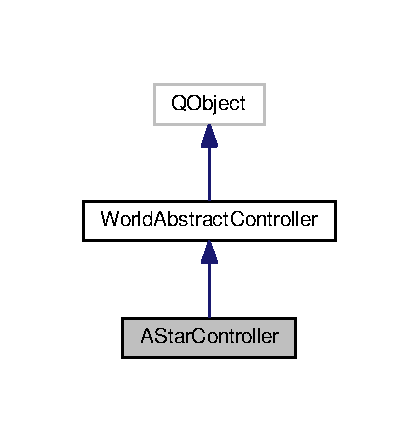
\includegraphics[width=201pt]{d5/dde/classAStarController__inherit__graph}
\end{center}
\end{figure}


Collaboration diagram for A\+Star\+Controller\+:\nopagebreak
\begin{figure}[H]
\begin{center}
\leavevmode
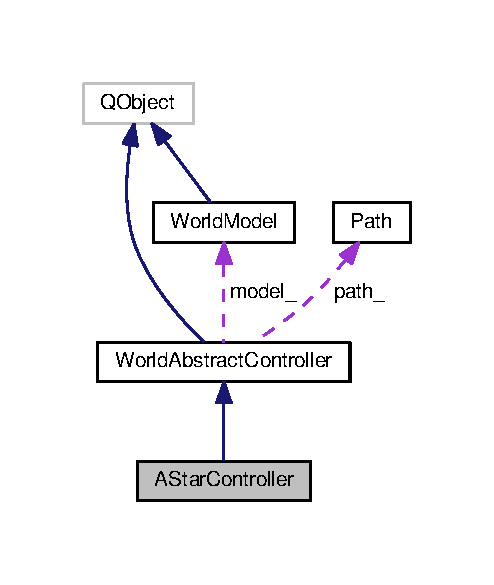
\includegraphics[width=237pt]{d1/dda/classAStarController__coll__graph}
\end{center}
\end{figure}
\subsection*{Public Member Functions}
\begin{DoxyCompactItemize}
\item 
\hyperlink{classAStarController_a098891ef3d828d56392e2e2ff48153b1}{A\+Star\+Controller} (\hyperlink{classWorldModel}{World\+Model} $\ast$model)
\begin{DoxyCompactList}\small\item\em Class constructor. \end{DoxyCompactList}\item 
virtual bool \hyperlink{classAStarController_aa230f8e80731d01daa502af943fe350e}{find\+Path} (const Q\+Point \&from, const Q\+Point \&to, float max\+Cost=I\+N\+F\+I\+N\+I\+TY) override
\begin{DoxyCompactList}\small\item\em Find the path to the position. \end{DoxyCompactList}\item 
virtual void \hyperlink{classAStarController_a228a9bd549dbae704ed6663ed726053e}{init} () override
\begin{DoxyCompactList}\small\item\em Initialization function. \end{DoxyCompactList}\item 
void \hyperlink{classAStarController_a002505340b1518995d830bc93e0ffd3d}{clear\+Nodes} ()\hypertarget{classAStarController_a002505340b1518995d830bc93e0ffd3d}{}\label{classAStarController_a002505340b1518995d830bc93e0ffd3d}

\begin{DoxyCompactList}\small\item\em Marks each node in node vector matrix as not visited. \end{DoxyCompactList}\end{DoxyCompactItemize}
\subsection*{Additional Inherited Members}


\subsection{Detailed Description}
A$\ast$ controller. 

This is the controller based on A$\ast$ path finding algorithm 

\subsection{Constructor \& Destructor Documentation}
\index{A\+Star\+Controller@{A\+Star\+Controller}!A\+Star\+Controller@{A\+Star\+Controller}}
\index{A\+Star\+Controller@{A\+Star\+Controller}!A\+Star\+Controller@{A\+Star\+Controller}}
\subsubsection[{\texorpdfstring{A\+Star\+Controller(\+World\+Model $\ast$model)}{AStarController(WorldModel *model)}}]{\setlength{\rightskip}{0pt plus 5cm}A\+Star\+Controller\+::\+A\+Star\+Controller (
\begin{DoxyParamCaption}
\item[{{\bf World\+Model} $\ast$}]{model}
\end{DoxyParamCaption}
)}\hypertarget{classAStarController_a098891ef3d828d56392e2e2ff48153b1}{}\label{classAStarController_a098891ef3d828d56392e2e2ff48153b1}


Class constructor. 


\begin{DoxyParams}{Parameters}
{\em model} & owner of the controller \\
\hline
\end{DoxyParams}


\subsection{Member Function Documentation}
\index{A\+Star\+Controller@{A\+Star\+Controller}!find\+Path@{find\+Path}}
\index{find\+Path@{find\+Path}!A\+Star\+Controller@{A\+Star\+Controller}}
\subsubsection[{\texorpdfstring{find\+Path(const Q\+Point \&from, const Q\+Point \&to, float max\+Cost=\+I\+N\+F\+I\+N\+I\+T\+Y) override}{findPath(const QPoint &from, const QPoint &to, float maxCost=INFINITY) override}}]{\setlength{\rightskip}{0pt plus 5cm}bool A\+Star\+Controller\+::find\+Path (
\begin{DoxyParamCaption}
\item[{const Q\+Point \&}]{from, }
\item[{const Q\+Point \&}]{to, }
\item[{float}]{max\+Cost = {\ttfamily INFINITY}}
\end{DoxyParamCaption}
)\hspace{0.3cm}{\ttfamily [override]}, {\ttfamily [virtual]}}\hypertarget{classAStarController_aa230f8e80731d01daa502af943fe350e}{}\label{classAStarController_aa230f8e80731d01daa502af943fe350e}


Find the path to the position. 

Find a path to the position using A$\ast$ algorithm 
\begin{DoxyParams}{Parameters}
{\em from} & starting point \\
\hline
{\em to} & destination \\
\hline
\end{DoxyParams}
\begin{DoxyReturn}{Returns}
true if the path was find, false otherwise 
\end{DoxyReturn}


Implements \hyperlink{classWorldAbstractController_a7716b59b6e3cbd086485e7012ae7d4f0}{World\+Abstract\+Controller}.

\index{A\+Star\+Controller@{A\+Star\+Controller}!init@{init}}
\index{init@{init}!A\+Star\+Controller@{A\+Star\+Controller}}
\subsubsection[{\texorpdfstring{init() override}{init() override}}]{\setlength{\rightskip}{0pt plus 5cm}void A\+Star\+Controller\+::init (
\begin{DoxyParamCaption}
{}
\end{DoxyParamCaption}
)\hspace{0.3cm}{\ttfamily [override]}, {\ttfamily [virtual]}}\hypertarget{classAStarController_a228a9bd549dbae704ed6663ed726053e}{}\label{classAStarController_a228a9bd549dbae704ed6663ed726053e}


Initialization function. 

Creates a node vector matrix from world\textquotesingle{}s tiles 

Implements \hyperlink{classWorldAbstractController_af2ab5103153a68f66dcdf75d6c9a4d93}{World\+Abstract\+Controller}.



The documentation for this class was generated from the following files\+:\begin{DoxyCompactItemize}
\item 
/home/bobiko/ku-\/leuven/media-\/processing/labs/finaltask/finaltask/src/controller/\hyperlink{astarcontroller_8h}{astarcontroller.\+h}\item 
/home/bobiko/ku-\/leuven/media-\/processing/labs/finaltask/finaltask/src/controller/\hyperlink{astarcontroller_8cpp}{astarcontroller.\+cpp}\end{DoxyCompactItemize}

\hypertarget{classCompareCost}{}\section{Compare\+Cost Class Reference}
\label{classCompareCost}\index{Compare\+Cost@{Compare\+Cost}}


\hyperlink{structNode}{Node} comparison functor.  




{\ttfamily \#include $<$astarcontroller.\+h$>$}

\subsection*{Public Member Functions}
\begin{DoxyCompactItemize}
\item 
bool {\bfseries operator()} (\hyperlink{structNode}{Node} $\ast$\&t1, \hyperlink{structNode}{Node} $\ast$\&t2) const \hypertarget{classCompareCost_adfeec8d428c577eab5d58c46dd692959}{}\label{classCompareCost_adfeec8d428c577eab5d58c46dd692959}

\end{DoxyCompactItemize}


\subsection{Detailed Description}
\hyperlink{structNode}{Node} comparison functor. 

Defines a more preferable node among two to prioritize in a queue 

The documentation for this class was generated from the following file\+:\begin{DoxyCompactItemize}
\item 
/home/bobiko/ku-\/leuven/media-\/processing/labs/finaltask/finaltask/src/controller/\hyperlink{astarcontroller_8h}{astarcontroller.\+h}\end{DoxyCompactItemize}

\hypertarget{classMainWindow}{}\section{Main\+Window Class Reference}
\label{classMainWindow}\index{Main\+Window@{Main\+Window}}


Main window of the application.  




{\ttfamily \#include $<$mainwindow.\+h$>$}



Inheritance diagram for Main\+Window\+:\nopagebreak
\begin{figure}[H]
\begin{center}
\leavevmode
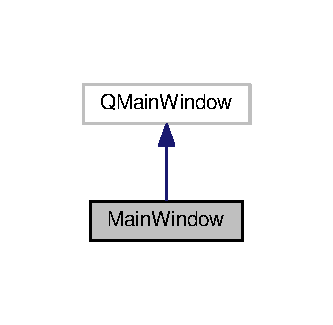
\includegraphics[width=160pt]{d1/d96/classMainWindow__inherit__graph}
\end{center}
\end{figure}


Collaboration diagram for Main\+Window\+:\nopagebreak
\begin{figure}[H]
\begin{center}
\leavevmode
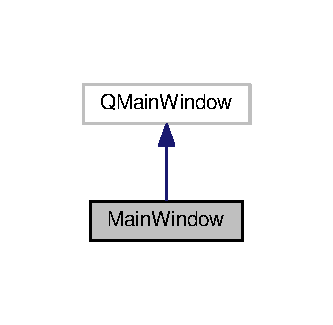
\includegraphics[width=160pt]{d2/d38/classMainWindow__coll__graph}
\end{center}
\end{figure}
\subsection*{Public Member Functions}
\begin{DoxyCompactItemize}
\item 
{\bfseries Main\+Window} (Q\+Widget $\ast$parent=0)\hypertarget{classMainWindow_a8b244be8b7b7db1b08de2a2acb9409db}{}\label{classMainWindow_a8b244be8b7b7db1b08de2a2acb9409db}

\item 
void \hyperlink{classMainWindow_a4b800fca70253ee8d6a38d8f435e5c10}{set\+Model} (\hyperlink{classWorldModel}{World\+Model} $\ast$m)
\begin{DoxyCompactList}\small\item\em Set model for both views. \end{DoxyCompactList}\end{DoxyCompactItemize}


\subsection{Detailed Description}
Main window of the application. 

The most part of implementation is done in Designer 

\subsection{Member Function Documentation}
\index{Main\+Window@{Main\+Window}!set\+Model@{set\+Model}}
\index{set\+Model@{set\+Model}!Main\+Window@{Main\+Window}}
\subsubsection[{\texorpdfstring{set\+Model(\+World\+Model $\ast$m)}{setModel(WorldModel *m)}}]{\setlength{\rightskip}{0pt plus 5cm}void Main\+Window\+::set\+Model (
\begin{DoxyParamCaption}
\item[{{\bf World\+Model} $\ast$}]{m}
\end{DoxyParamCaption}
)}\hypertarget{classMainWindow_a4b800fca70253ee8d6a38d8f435e5c10}{}\label{classMainWindow_a4b800fca70253ee8d6a38d8f435e5c10}


Set model for both views. 


\begin{DoxyParams}{Parameters}
{\em m} & model \\
\hline
\end{DoxyParams}


The documentation for this class was generated from the following files\+:\begin{DoxyCompactItemize}
\item 
/home/bobiko/ku-\/leuven/media-\/processing/labs/finaltask/finaltask/src/mainui/\hyperlink{mainwindow_8h}{mainwindow.\+h}\item 
/home/bobiko/ku-\/leuven/media-\/processing/labs/finaltask/finaltask/src/mainui/\hyperlink{mainwindow_8cpp}{mainwindow.\+cpp}\end{DoxyCompactItemize}

\hypertarget{structNode}{}\section{Node Struct Reference}
\label{structNode}\index{Node@{Node}}


The \hyperlink{structNode}{Node} struct.  




{\ttfamily \#include $<$astarcontroller.\+h$>$}



Collaboration diagram for Node\+:
\nopagebreak
\begin{figure}[H]
\begin{center}
\leavevmode
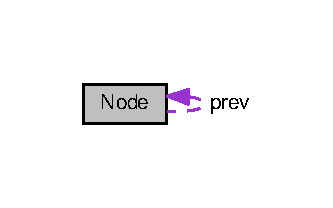
\includegraphics[width=160pt]{d6/d2c/structNode__coll__graph}
\end{center}
\end{figure}
\subsection*{Public Attributes}
\begin{DoxyCompactItemize}
\item 
bool {\bfseries visited}\hypertarget{structNode_aa1bdec4e775fc578632e6a2dced9e251}{}\label{structNode_aa1bdec4e775fc578632e6a2dced9e251}

\item 
float {\bfseries node\+Cost}\hypertarget{structNode_a4b2a95877effb35a6a80d12af0bee8ee}{}\label{structNode_a4b2a95877effb35a6a80d12af0bee8ee}

\item 
float {\bfseries g}\hypertarget{structNode_a914881afe2945fb2e60eb68a6c223d30}{}\label{structNode_a914881afe2945fb2e60eb68a6c223d30}

\item 
float {\bfseries h}\hypertarget{structNode_ab7d8a0250a536b3b221dd6d42e7630e0}{}\label{structNode_ab7d8a0250a536b3b221dd6d42e7630e0}

\item 
float {\bfseries f}\hypertarget{structNode_ad16e9a3090431644ea3283b07c91a6a4}{}\label{structNode_ad16e9a3090431644ea3283b07c91a6a4}

\item 
int {\bfseries x}\hypertarget{structNode_aff1029a518bdc2651007b8856f958364}{}\label{structNode_aff1029a518bdc2651007b8856f958364}

\item 
int {\bfseries y}\hypertarget{structNode_aa3e5b5240023b4528ae85057b3324202}{}\label{structNode_aa3e5b5240023b4528ae85057b3324202}

\item 
std\+::array$<$ \hyperlink{structNode}{Node} $\ast$, 4 $>$ {\bfseries neighbours}\hypertarget{structNode_a44d1de666d130924725a2a7c42daacc4}{}\label{structNode_a44d1de666d130924725a2a7c42daacc4}

\item 
\hyperlink{structNode}{Node} $\ast$ {\bfseries prev}\hypertarget{structNode_a632ea91c6a13082308f7692649a68880}{}\label{structNode_a632ea91c6a13082308f7692649a68880}

\end{DoxyCompactItemize}


\subsection{Detailed Description}
The \hyperlink{structNode}{Node} struct. 

Contains information about tiles visit flag, energy costs, postion, pointers to its neigbours and predicessors 

The documentation for this struct was generated from the following file\+:\begin{DoxyCompactItemize}
\item 
/home/bobiko/ku-\/leuven/media-\/processing/labs/finaltask/finaltask/src/controller/\hyperlink{astarcontroller_8h}{astarcontroller.\+h}\end{DoxyCompactItemize}

\hypertarget{structPath}{}\section{Path Struct Reference}
\label{structPath}\index{Path@{Path}}


The \hyperlink{structPath}{Path} struct.  




{\ttfamily \#include $<$worldabstractcontroller.\+h$>$}

\subsection*{Public Attributes}
\begin{DoxyCompactItemize}
\item 
double {\bfseries cost}\hypertarget{structPath_a4d54acc172b9690ba67bebec88c9d2c6}{}\label{structPath_a4d54acc172b9690ba67bebec88c9d2c6}

\item 
Q\+Vector$<$ Q\+Point $>$ {\bfseries steps}\hypertarget{structPath_a4be65f498114d6bf65f8934c2bb180eb}{}\label{structPath_a4be65f498114d6bf65f8934c2bb180eb}

\end{DoxyCompactItemize}


\subsection{Detailed Description}
The \hyperlink{structPath}{Path} struct. 

Includes vector of steps to perform and overall energy cost 

The documentation for this struct was generated from the following file\+:\begin{DoxyCompactItemize}
\item 
/home/bobiko/ku-\/leuven/media-\/processing/labs/finaltask/finaltask/src/controller/\hyperlink{worldabstractcontroller_8h}{worldabstractcontroller.\+h}\end{DoxyCompactItemize}

\hypertarget{classPopup}{}\section{Popup Class Reference}
\label{classPopup}\index{Popup@{Popup}}


Stratup dialog class.  




{\ttfamily \#include $<$popup.\+h$>$}



Inheritance diagram for Popup\+:\nopagebreak
\begin{figure}[H]
\begin{center}
\leavevmode
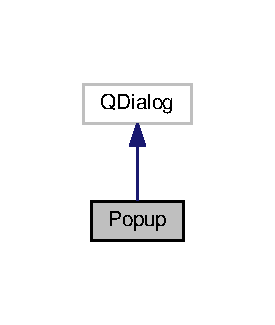
\includegraphics[width=132pt]{d3/dac/classPopup__inherit__graph}
\end{center}
\end{figure}


Collaboration diagram for Popup\+:\nopagebreak
\begin{figure}[H]
\begin{center}
\leavevmode
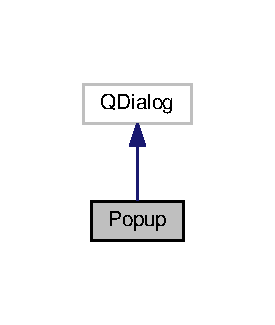
\includegraphics[width=132pt]{d2/dba/classPopup__coll__graph}
\end{center}
\end{figure}
\subsection*{Public Member Functions}
\begin{DoxyCompactItemize}
\item 
{\bfseries Popup} (Q\+Dialog $\ast$parent=nullptr)\hypertarget{classPopup_ae485ca6139d79feabf12322369e7ecbc}{}\label{classPopup_ae485ca6139d79feabf12322369e7ecbc}

\item 
\hyperlink{structValues}{Values} \hyperlink{classPopup_a7db1e47b567d26051a5dd40d1c14dd89}{get\+Values} ()\hypertarget{classPopup_a7db1e47b567d26051a5dd40d1c14dd89}{}\label{classPopup_a7db1e47b567d26051a5dd40d1c14dd89}

\begin{DoxyCompactList}\small\item\em Returns values of \hyperlink{classPopup}{Popup} controls. \end{DoxyCompactList}\end{DoxyCompactItemize}


\subsection{Detailed Description}
Stratup dialog class. 

Allows user to pick the map, number of enemies and health packs and optimization level of the controller 

The documentation for this class was generated from the following files\+:\begin{DoxyCompactItemize}
\item 
/home/bobiko/ku-\/leuven/media-\/processing/labs/finaltask/finaltask/src/mainui/\hyperlink{popup_8h}{popup.\+h}\item 
/home/bobiko/ku-\/leuven/media-\/processing/labs/finaltask/finaltask/src/mainui/\hyperlink{popup_8cpp}{popup.\+cpp}\end{DoxyCompactItemize}

\hypertarget{classUEnemy}{}\section{U\+Enemy Class Reference}
\label{classUEnemy}\index{U\+Enemy@{U\+Enemy}}


Updated enemy class.  




{\ttfamily \#include $<$uworld.\+h$>$}



Inheritance diagram for U\+Enemy\+:
\nopagebreak
\begin{figure}[H]
\begin{center}
\leavevmode
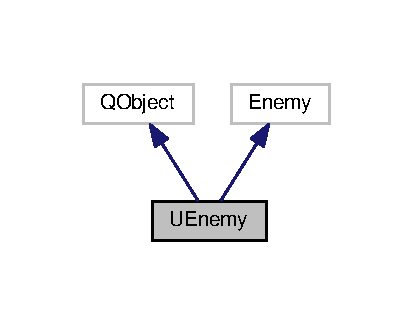
\includegraphics[width=198pt]{da/d90/classUEnemy__inherit__graph}
\end{center}
\end{figure}


Collaboration diagram for U\+Enemy\+:
\nopagebreak
\begin{figure}[H]
\begin{center}
\leavevmode
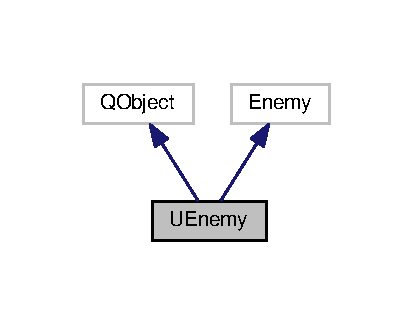
\includegraphics[width=198pt]{d5/d7a/classUEnemy__coll__graph}
\end{center}
\end{figure}
\subsection*{Signals}
\begin{DoxyCompactItemize}
\item 
void \hyperlink{classUEnemy_aa00c76b00d33570ade0136e60beaf9a5}{dead} ()\hypertarget{classUEnemy_aa00c76b00d33570ade0136e60beaf9a5}{}\label{classUEnemy_aa00c76b00d33570ade0136e60beaf9a5}

\begin{DoxyCompactList}\small\item\em Emited once enemy is defeated. \end{DoxyCompactList}\end{DoxyCompactItemize}
\subsection*{Public Member Functions}
\begin{DoxyCompactItemize}
\item 
\hyperlink{classUEnemy_a68c1fd174c1fafe929056d1899bdef49}{U\+Enemy} (int x\+Position, int y\+Position, float strength, int radius=5)
\begin{DoxyCompactList}\small\item\em Class constructor. \end{DoxyCompactList}\item 
float \hyperlink{classUEnemy_a2295a17437a57c677320f5e501fa0474}{attack} ()
\begin{DoxyCompactList}\small\item\em Attack the enemy. \end{DoxyCompactList}\item 
const Q\+Rect \& \hyperlink{classUEnemy_ab89322d753c29076f7f0b0715a87a62a}{area} () const \hypertarget{classUEnemy_ab89322d753c29076f7f0b0715a87a62a}{}\label{classUEnemy_ab89322d753c29076f7f0b0715a87a62a}

\begin{DoxyCompactList}\small\item\em Returns area occupied by the object. \end{DoxyCompactList}\end{DoxyCompactItemize}


\subsection{Detailed Description}
Updated enemy class. 

\subsection{Constructor \& Destructor Documentation}
\index{U\+Enemy@{U\+Enemy}!U\+Enemy@{U\+Enemy}}
\index{U\+Enemy@{U\+Enemy}!U\+Enemy@{U\+Enemy}}
\subsubsection[{\texorpdfstring{U\+Enemy(int x\+Position, int y\+Position, float strength, int radius=5)}{UEnemy(int xPosition, int yPosition, float strength, int radius=5)}}]{\setlength{\rightskip}{0pt plus 5cm}U\+Enemy\+::\+U\+Enemy (
\begin{DoxyParamCaption}
\item[{int}]{x\+Position, }
\item[{int}]{y\+Position, }
\item[{float}]{strength, }
\item[{int}]{radius = {\ttfamily 5}}
\end{DoxyParamCaption}
)\hspace{0.3cm}{\ttfamily [explicit]}}\hypertarget{classUEnemy_a68c1fd174c1fafe929056d1899bdef49}{}\label{classUEnemy_a68c1fd174c1fafe929056d1899bdef49}


Class constructor. 


\begin{DoxyParams}{Parameters}
{\em x} & horizontal position \\
\hline
{\em y} & vertical position \\
\hline
{\em strength} & damage to be caused \\
\hline
{\em radius} & radius of occupied area in pixels \\
\hline
\end{DoxyParams}


\subsection{Member Function Documentation}
\index{U\+Enemy@{U\+Enemy}!attack@{attack}}
\index{attack@{attack}!U\+Enemy@{U\+Enemy}}
\subsubsection[{\texorpdfstring{attack()}{attack()}}]{\setlength{\rightskip}{0pt plus 5cm}float U\+Enemy\+::attack (
\begin{DoxyParamCaption}
{}
\end{DoxyParamCaption}
)}\hypertarget{classUEnemy_a2295a17437a57c677320f5e501fa0474}{}\label{classUEnemy_a2295a17437a57c677320f5e501fa0474}


Attack the enemy. 

Emits dead signal and returns the damage to be caused \begin{DoxyReturn}{Returns}
damage to be caused 
\end{DoxyReturn}


The documentation for this class was generated from the following files\+:\begin{DoxyCompactItemize}
\item 
/home/bobiko/ku-\/leuven/media-\/processing/labs/finaltask/finaltask/src/libworld-\/update/\hyperlink{uworld_8h}{uworld.\+h}\item 
/home/bobiko/ku-\/leuven/media-\/processing/labs/finaltask/finaltask/src/libworld-\/update/\hyperlink{uworld_8cpp}{uworld.\+cpp}\end{DoxyCompactItemize}

\hypertarget{classUHealthPack}{}\section{U\+Health\+Pack Class Reference}
\label{classUHealthPack}\index{U\+Health\+Pack@{U\+Health\+Pack}}


Updated health pack class.  




{\ttfamily \#include $<$uworld.\+h$>$}



Inheritance diagram for U\+Health\+Pack\+:\nopagebreak
\begin{figure}[H]
\begin{center}
\leavevmode
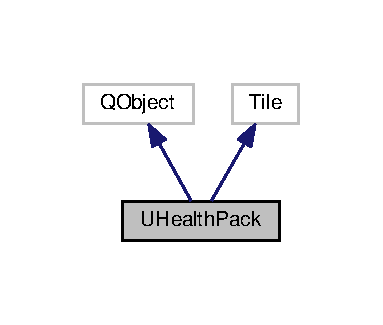
\includegraphics[width=184pt]{d5/dd8/classUHealthPack__inherit__graph}
\end{center}
\end{figure}


Collaboration diagram for U\+Health\+Pack\+:\nopagebreak
\begin{figure}[H]
\begin{center}
\leavevmode
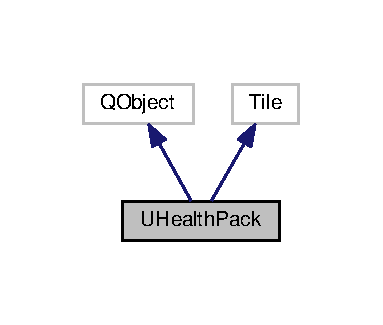
\includegraphics[width=184pt]{df/da1/classUHealthPack__coll__graph}
\end{center}
\end{figure}
\subsection*{Signals}
\begin{DoxyCompactItemize}
\item 
void \hyperlink{classUHealthPack_a1f5645d92da31de8300ad6885875cf92}{used} ()\hypertarget{classUHealthPack_a1f5645d92da31de8300ad6885875cf92}{}\label{classUHealthPack_a1f5645d92da31de8300ad6885875cf92}

\begin{DoxyCompactList}\small\item\em Healthpack was used signal. \end{DoxyCompactList}\end{DoxyCompactItemize}
\subsection*{Public Member Functions}
\begin{DoxyCompactItemize}
\item 
\hyperlink{classUHealthPack_a03ddd3ed3c03bc8b342807b73eb01c49}{U\+Health\+Pack} (int x, int y, float health\+Points)
\begin{DoxyCompactList}\small\item\em Class constructor. \end{DoxyCompactList}\item 
float \hyperlink{classUHealthPack_a19dd8468b98963e293940db3020f9b9d}{use} ()
\begin{DoxyCompactList}\small\item\em Use healthpack. \end{DoxyCompactList}\item 
const Q\+Rect \& \hyperlink{classUHealthPack_a375be70224cbeb112cbcfe9ff76ed700}{area} () const \hypertarget{classUHealthPack_a375be70224cbeb112cbcfe9ff76ed700}{}\label{classUHealthPack_a375be70224cbeb112cbcfe9ff76ed700}

\begin{DoxyCompactList}\small\item\em Returns area occupied by the object. \end{DoxyCompactList}\end{DoxyCompactItemize}


\subsection{Detailed Description}
Updated health pack class. 

\subsection{Constructor \& Destructor Documentation}
\index{U\+Health\+Pack@{U\+Health\+Pack}!U\+Health\+Pack@{U\+Health\+Pack}}
\index{U\+Health\+Pack@{U\+Health\+Pack}!U\+Health\+Pack@{U\+Health\+Pack}}
\subsubsection[{\texorpdfstring{U\+Health\+Pack(int x, int y, float health\+Points)}{UHealthPack(int x, int y, float healthPoints)}}]{\setlength{\rightskip}{0pt plus 5cm}U\+Health\+Pack\+::\+U\+Health\+Pack (
\begin{DoxyParamCaption}
\item[{int}]{x, }
\item[{int}]{y, }
\item[{float}]{health\+Points}
\end{DoxyParamCaption}
)}\hypertarget{classUHealthPack_a03ddd3ed3c03bc8b342807b73eb01c49}{}\label{classUHealthPack_a03ddd3ed3c03bc8b342807b73eb01c49}


Class constructor. 


\begin{DoxyParams}{Parameters}
{\em x} & horizontal position \\
\hline
{\em y} & vertical position \\
\hline
{\em health\+Points} & HP to be restored \\
\hline
{\em radius} & radius of occupied area in pixels \\
\hline
\end{DoxyParams}


\subsection{Member Function Documentation}
\index{U\+Health\+Pack@{U\+Health\+Pack}!use@{use}}
\index{use@{use}!U\+Health\+Pack@{U\+Health\+Pack}}
\subsubsection[{\texorpdfstring{use()}{use()}}]{\setlength{\rightskip}{0pt plus 5cm}float U\+Health\+Pack\+::use (
\begin{DoxyParamCaption}
{}
\end{DoxyParamCaption}
)}\hypertarget{classUHealthPack_a19dd8468b98963e293940db3020f9b9d}{}\label{classUHealthPack_a19dd8468b98963e293940db3020f9b9d}


Use healthpack. 

Emits the signal that the health pack is used and returns HP to be restored \begin{DoxyReturn}{Returns}
HP to be restored 
\end{DoxyReturn}


The documentation for this class was generated from the following files\+:\begin{DoxyCompactItemize}
\item 
/home/bobiko/ku-\/leuven/media-\/processing/labs/finaltask/finaltask/src/libworld-\/update/\hyperlink{uworld_8h}{uworld.\+h}\item 
/home/bobiko/ku-\/leuven/media-\/processing/labs/finaltask/finaltask/src/libworld-\/update/\hyperlink{uworld_8cpp}{uworld.\+cpp}\end{DoxyCompactItemize}

\hypertarget{classUPEnemy}{}\section{U\+P\+Enemy Class Reference}
\label{classUPEnemy}\index{U\+P\+Enemy@{U\+P\+Enemy}}


Updated poisoned enemy class.  




{\ttfamily \#include $<$uworld.\+h$>$}



Inheritance diagram for U\+P\+Enemy\+:\nopagebreak
\begin{figure}[H]
\begin{center}
\leavevmode
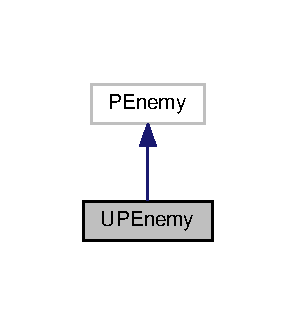
\includegraphics[width=142pt]{da/dff/classUPEnemy__inherit__graph}
\end{center}
\end{figure}


Collaboration diagram for U\+P\+Enemy\+:\nopagebreak
\begin{figure}[H]
\begin{center}
\leavevmode
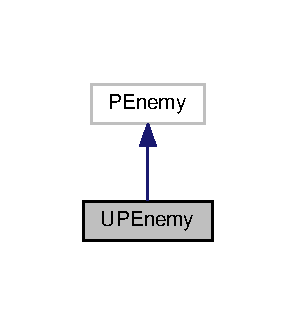
\includegraphics[width=142pt]{d3/dfe/classUPEnemy__coll__graph}
\end{center}
\end{figure}
\subsection*{Signals}
\begin{DoxyCompactItemize}
\item 
void \hyperlink{classUPEnemy_ac021d11a175d2f07c2055a4c8aace52d}{area\+Poisoned} (int value, Q\+Rect \hyperlink{classUPEnemy_aa87ac038b30dccbad0a0966824d99382}{area})
\begin{DoxyCompactList}\small\item\em Poison the area signal. \end{DoxyCompactList}\end{DoxyCompactItemize}
\subsection*{Public Member Functions}
\begin{DoxyCompactItemize}
\item 
\hyperlink{classUPEnemy_a118be97fa267047357fb56571eaef1ed}{U\+P\+Enemy} (int x, int y, float strength)
\begin{DoxyCompactList}\small\item\em Class constructor. \end{DoxyCompactList}\item 
const Q\+Rect \& \hyperlink{classUPEnemy_aa87ac038b30dccbad0a0966824d99382}{area} ()\hypertarget{classUPEnemy_aa87ac038b30dccbad0a0966824d99382}{}\label{classUPEnemy_aa87ac038b30dccbad0a0966824d99382}

\begin{DoxyCompactList}\small\item\em Returns area occupied by the object. \end{DoxyCompactList}\item 
const Q\+Rect \& \hyperlink{classUPEnemy_a88cc91ecae7705053e6cfbab57f60503}{poison\+Area} ()\hypertarget{classUPEnemy_a88cc91ecae7705053e6cfbab57f60503}{}\label{classUPEnemy_a88cc91ecae7705053e6cfbab57f60503}

\begin{DoxyCompactList}\small\item\em Returns poison area of the enemy. \end{DoxyCompactList}\item 
void \hyperlink{classUPEnemy_aa1145894e8e7c203796e653309fdb661}{attack} ()
\begin{DoxyCompactList}\small\item\em Attack the enemy. \end{DoxyCompactList}\item 
bool \hyperlink{classUPEnemy_a4a3e30df0c5f369a4859803970d5e69c}{is\+Triggered} () const \hypertarget{classUPEnemy_a4a3e30df0c5f369a4859803970d5e69c}{}\label{classUPEnemy_a4a3e30df0c5f369a4859803970d5e69c}

\begin{DoxyCompactList}\small\item\em Check if the enemy has been already attacked. \end{DoxyCompactList}\end{DoxyCompactItemize}


\subsection{Detailed Description}
Updated poisoned enemy class. 

\subsection{Constructor \& Destructor Documentation}
\index{U\+P\+Enemy@{U\+P\+Enemy}!U\+P\+Enemy@{U\+P\+Enemy}}
\index{U\+P\+Enemy@{U\+P\+Enemy}!U\+P\+Enemy@{U\+P\+Enemy}}
\subsubsection[{\texorpdfstring{U\+P\+Enemy(int x, int y, float strength)}{UPEnemy(int x, int y, float strength)}}]{\setlength{\rightskip}{0pt plus 5cm}U\+P\+Enemy\+::\+U\+P\+Enemy (
\begin{DoxyParamCaption}
\item[{int}]{x, }
\item[{int}]{y, }
\item[{float}]{strength}
\end{DoxyParamCaption}
)}\hypertarget{classUPEnemy_a118be97fa267047357fb56571eaef1ed}{}\label{classUPEnemy_a118be97fa267047357fb56571eaef1ed}


Class constructor. 


\begin{DoxyParams}{Parameters}
{\em x} & horizontal position \\
\hline
{\em y} & vertical position \\
\hline
{\em strength} & damage to be caused \\
\hline
{\em radius} & radius of occupied area in pixels \\
\hline
\end{DoxyParams}


\subsection{Member Function Documentation}
\index{U\+P\+Enemy@{U\+P\+Enemy}!area\+Poisoned@{area\+Poisoned}}
\index{area\+Poisoned@{area\+Poisoned}!U\+P\+Enemy@{U\+P\+Enemy}}
\subsubsection[{\texorpdfstring{area\+Poisoned}{areaPoisoned}}]{\setlength{\rightskip}{0pt plus 5cm}void U\+P\+Enemy\+::area\+Poisoned (
\begin{DoxyParamCaption}
\item[{int}]{value, }
\item[{Q\+Rect}]{area}
\end{DoxyParamCaption}
)\hspace{0.3cm}{\ttfamily [signal]}}\hypertarget{classUPEnemy_ac021d11a175d2f07c2055a4c8aace52d}{}\label{classUPEnemy_ac021d11a175d2f07c2055a4c8aace52d}


Poison the area signal. 


\begin{DoxyParams}{Parameters}
{\em value} & poison level \\
\hline
{\em area} & poisoned area \\
\hline
\end{DoxyParams}
\index{U\+P\+Enemy@{U\+P\+Enemy}!attack@{attack}}
\index{attack@{attack}!U\+P\+Enemy@{U\+P\+Enemy}}
\subsubsection[{\texorpdfstring{attack()}{attack()}}]{\setlength{\rightskip}{0pt plus 5cm}void U\+P\+Enemy\+::attack (
\begin{DoxyParamCaption}
{}
\end{DoxyParamCaption}
)}\hypertarget{classUPEnemy_aa1145894e8e7c203796e653309fdb661}{}\label{classUPEnemy_aa1145894e8e7c203796e653309fdb661}


Attack the enemy. 

Triggers the posioning process 

The documentation for this class was generated from the following files\+:\begin{DoxyCompactItemize}
\item 
/home/bobiko/ku-\/leuven/media-\/processing/labs/finaltask/finaltask/src/libworld-\/update/\hyperlink{uworld_8h}{uworld.\+h}\item 
/home/bobiko/ku-\/leuven/media-\/processing/labs/finaltask/finaltask/src/libworld-\/update/\hyperlink{uworld_8cpp}{uworld.\+cpp}\end{DoxyCompactItemize}

\hypertarget{classUProtagonist}{}\section{U\+Protagonist Class Reference}
\label{classUProtagonist}\index{U\+Protagonist@{U\+Protagonist}}


Updated protagonist class.  




{\ttfamily \#include $<$uworld.\+h$>$}



Inheritance diagram for U\+Protagonist\+:\nopagebreak
\begin{figure}[H]
\begin{center}
\leavevmode
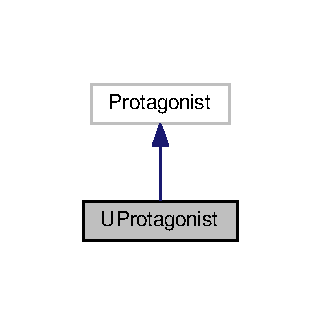
\includegraphics[width=154pt]{d8/da2/classUProtagonist__inherit__graph}
\end{center}
\end{figure}


Collaboration diagram for U\+Protagonist\+:\nopagebreak
\begin{figure}[H]
\begin{center}
\leavevmode
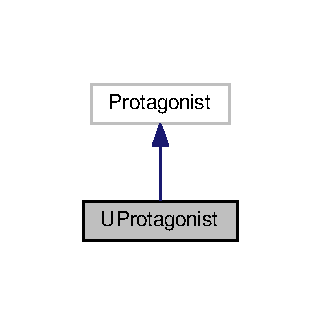
\includegraphics[width=154pt]{df/d4d/classUProtagonist__coll__graph}
\end{center}
\end{figure}
\subsection*{Public Slots}
\begin{DoxyCompactItemize}
\item 
void \hyperlink{classUProtagonist_aafceebba330665d6c8cf6943515526d5}{restore\+Energy} ()\hypertarget{classUProtagonist_aafceebba330665d6c8cf6943515526d5}{}\label{classUProtagonist_aafceebba330665d6c8cf6943515526d5}

\begin{DoxyCompactList}\small\item\em Completely restore the energy level. \end{DoxyCompactList}\end{DoxyCompactItemize}
\subsection*{Signals}
\begin{DoxyCompactItemize}
\item 
void \hyperlink{classUProtagonist_a51cf4f46d0b8d841ac91fb26cd175f04}{health\+Level\+Changed} (int value)
\begin{DoxyCompactList}\small\item\em Health changed signal. \end{DoxyCompactList}\item 
void \hyperlink{classUProtagonist_a5f04fffdddf19813626e2676152425d9}{energy\+Level\+Changed} (int value)
\begin{DoxyCompactList}\small\item\em Energy changed signal. \end{DoxyCompactList}\item 
void \hyperlink{classUProtagonist_ade87a2c665976c4e46991e6aa9e41875}{poisoned} ()\hypertarget{classUProtagonist_ade87a2c665976c4e46991e6aa9e41875}{}\label{classUProtagonist_ade87a2c665976c4e46991e6aa9e41875}

\begin{DoxyCompactList}\small\item\em Signal to be emitted every time the hero is poisoned. \end{DoxyCompactList}\end{DoxyCompactItemize}
\subsection*{Public Member Functions}
\begin{DoxyCompactItemize}
\item 
\hyperlink{classUProtagonist_aecc46a5d2ad349f141f7d623b6454816}{U\+Protagonist} (int radius=5)
\begin{DoxyCompactList}\small\item\em Class constructor. \end{DoxyCompactList}\item 
void \hyperlink{classUProtagonist_a453bac1fc034e1c15ad8d7bdac566421}{update\+Health} (float diff)
\begin{DoxyCompactList}\small\item\em Update health. \end{DoxyCompactList}\item 
void \hyperlink{classUProtagonist_a56f48e2a59eca29575cac673a03cbd69}{update\+Energy} (float diff)
\begin{DoxyCompactList}\small\item\em Update energy. \end{DoxyCompactList}\item 
const Q\+Rect \& \hyperlink{classUProtagonist_ae564263d78b9c1e15a27392376b1c2b3}{area} () const \hypertarget{classUProtagonist_ae564263d78b9c1e15a27392376b1c2b3}{}\label{classUProtagonist_ae564263d78b9c1e15a27392376b1c2b3}

\begin{DoxyCompactList}\small\item\em Returns area occupied by the object. \end{DoxyCompactList}\item 
void \hyperlink{classUProtagonist_a367f9c57f2b80bcc088d8cc2f88037a4}{poison} (float damage)
\begin{DoxyCompactList}\small\item\em Poison the enemy. \end{DoxyCompactList}\end{DoxyCompactItemize}


\subsection{Detailed Description}
Updated protagonist class. 

\subsection{Constructor \& Destructor Documentation}
\index{U\+Protagonist@{U\+Protagonist}!U\+Protagonist@{U\+Protagonist}}
\index{U\+Protagonist@{U\+Protagonist}!U\+Protagonist@{U\+Protagonist}}
\subsubsection[{\texorpdfstring{U\+Protagonist(int radius=5)}{UProtagonist(int radius=5)}}]{\setlength{\rightskip}{0pt plus 5cm}U\+Protagonist\+::\+U\+Protagonist (
\begin{DoxyParamCaption}
\item[{int}]{radius = {\ttfamily 5}}
\end{DoxyParamCaption}
)}\hypertarget{classUProtagonist_aecc46a5d2ad349f141f7d623b6454816}{}\label{classUProtagonist_aecc46a5d2ad349f141f7d623b6454816}


Class constructor. 


\begin{DoxyParams}{Parameters}
{\em radius} & radius occupied by the object \\
\hline
\end{DoxyParams}


\subsection{Member Function Documentation}
\index{U\+Protagonist@{U\+Protagonist}!energy\+Level\+Changed@{energy\+Level\+Changed}}
\index{energy\+Level\+Changed@{energy\+Level\+Changed}!U\+Protagonist@{U\+Protagonist}}
\subsubsection[{\texorpdfstring{energy\+Level\+Changed}{energyLevelChanged}}]{\setlength{\rightskip}{0pt plus 5cm}void U\+Protagonist\+::energy\+Level\+Changed (
\begin{DoxyParamCaption}
\item[{int}]{value}
\end{DoxyParamCaption}
)\hspace{0.3cm}{\ttfamily [signal]}}\hypertarget{classUProtagonist_a5f04fffdddf19813626e2676152425d9}{}\label{classUProtagonist_a5f04fffdddf19813626e2676152425d9}


Energy changed signal. 

\begin{DoxySeeAlso}{See also}
\hyperlink{classUProtagonist_a56f48e2a59eca29575cac673a03cbd69}{update\+Energy} 
\end{DoxySeeAlso}

\begin{DoxyParams}{Parameters}
{\em value} & current energy level \\
\hline
\end{DoxyParams}
\index{U\+Protagonist@{U\+Protagonist}!health\+Level\+Changed@{health\+Level\+Changed}}
\index{health\+Level\+Changed@{health\+Level\+Changed}!U\+Protagonist@{U\+Protagonist}}
\subsubsection[{\texorpdfstring{health\+Level\+Changed}{healthLevelChanged}}]{\setlength{\rightskip}{0pt plus 5cm}void U\+Protagonist\+::health\+Level\+Changed (
\begin{DoxyParamCaption}
\item[{int}]{value}
\end{DoxyParamCaption}
)\hspace{0.3cm}{\ttfamily [signal]}}\hypertarget{classUProtagonist_a51cf4f46d0b8d841ac91fb26cd175f04}{}\label{classUProtagonist_a51cf4f46d0b8d841ac91fb26cd175f04}


Health changed signal. 

\begin{DoxySeeAlso}{See also}
\hyperlink{classUProtagonist_a453bac1fc034e1c15ad8d7bdac566421}{update\+Health} 
\end{DoxySeeAlso}

\begin{DoxyParams}{Parameters}
{\em value} & current health level \\
\hline
\end{DoxyParams}
\index{U\+Protagonist@{U\+Protagonist}!poison@{poison}}
\index{poison@{poison}!U\+Protagonist@{U\+Protagonist}}
\subsubsection[{\texorpdfstring{poison(float damage)}{poison(float damage)}}]{\setlength{\rightskip}{0pt plus 5cm}void U\+Protagonist\+::poison (
\begin{DoxyParamCaption}
\item[{float}]{damage}
\end{DoxyParamCaption}
)}\hypertarget{classUProtagonist_a367f9c57f2b80bcc088d8cc2f88037a4}{}\label{classUProtagonist_a367f9c57f2b80bcc088d8cc2f88037a4}


Poison the enemy. 

Decreases protagonist\textquotesingle{}s health and emits \hyperlink{classUProtagonist_ade87a2c665976c4e46991e6aa9e41875}{poisoned()} signal 
\begin{DoxyParams}{Parameters}
{\em damage} & HP to decrease \\
\hline
\end{DoxyParams}
\index{U\+Protagonist@{U\+Protagonist}!update\+Energy@{update\+Energy}}
\index{update\+Energy@{update\+Energy}!U\+Protagonist@{U\+Protagonist}}
\subsubsection[{\texorpdfstring{update\+Energy(float diff)}{updateEnergy(float diff)}}]{\setlength{\rightskip}{0pt plus 5cm}void U\+Protagonist\+::update\+Energy (
\begin{DoxyParamCaption}
\item[{float}]{diff}
\end{DoxyParamCaption}
)}\hypertarget{classUProtagonist_a56f48e2a59eca29575cac673a03cbd69}{}\label{classUProtagonist_a56f48e2a59eca29575cac673a03cbd69}


Update energy. 

\begin{DoxySeeAlso}{See also}
\hyperlink{classUProtagonist_a5f04fffdddf19813626e2676152425d9}{energy\+Level\+Changed} 
\end{DoxySeeAlso}

\begin{DoxyParams}{Parameters}
{\em diff} & EP to be added \\
\hline
\end{DoxyParams}
\index{U\+Protagonist@{U\+Protagonist}!update\+Health@{update\+Health}}
\index{update\+Health@{update\+Health}!U\+Protagonist@{U\+Protagonist}}
\subsubsection[{\texorpdfstring{update\+Health(float diff)}{updateHealth(float diff)}}]{\setlength{\rightskip}{0pt plus 5cm}void U\+Protagonist\+::update\+Health (
\begin{DoxyParamCaption}
\item[{float}]{diff}
\end{DoxyParamCaption}
)}\hypertarget{classUProtagonist_a453bac1fc034e1c15ad8d7bdac566421}{}\label{classUProtagonist_a453bac1fc034e1c15ad8d7bdac566421}


Update health. 

\begin{DoxySeeAlso}{See also}
\hyperlink{classUProtagonist_a51cf4f46d0b8d841ac91fb26cd175f04}{health\+Level\+Changed} 
\end{DoxySeeAlso}

\begin{DoxyParams}{Parameters}
{\em diff} & HP to be added \\
\hline
\end{DoxyParams}


The documentation for this class was generated from the following files\+:\begin{DoxyCompactItemize}
\item 
/home/bobiko/ku-\/leuven/media-\/processing/labs/finaltask/finaltask/src/libworld-\/update/\hyperlink{uworld_8h}{uworld.\+h}\item 
/home/bobiko/ku-\/leuven/media-\/processing/labs/finaltask/finaltask/src/libworld-\/update/\hyperlink{uworld_8cpp}{uworld.\+cpp}\end{DoxyCompactItemize}

\hypertarget{classUWorld}{}\section{U\+World Class Reference}
\label{classUWorld}\index{U\+World@{U\+World}}


Updated world class.  




{\ttfamily \#include $<$uworld.\+h$>$}

\subsection*{Public Member Functions}
\begin{DoxyCompactItemize}
\item 
\hyperlink{classUWorld_a4336a8896885a7ce345b13a142902dd5}{U\+World} (Q\+String filename)
\begin{DoxyCompactList}\small\item\em Class constructor. \end{DoxyCompactList}\item 
const std\+::vector$<$ std\+::unique\+\_\+ptr$<$ Tile $>$ $>$ \& \hyperlink{classUWorld_a5903b82b41401b80f6f0a7b10f4a7f9e}{get\+Map} () const \hypertarget{classUWorld_a5903b82b41401b80f6f0a7b10f4a7f9e}{}\label{classUWorld_a5903b82b41401b80f6f0a7b10f4a7f9e}

\begin{DoxyCompactList}\small\item\em Return map tiles. \end{DoxyCompactList}\item 
int \hyperlink{classUWorld_a4664a9e8e2b77b3f5be4674a81c09519}{get\+Cols} () const \hypertarget{classUWorld_a4664a9e8e2b77b3f5be4674a81c09519}{}\label{classUWorld_a4664a9e8e2b77b3f5be4674a81c09519}

\begin{DoxyCompactList}\small\item\em Return number of columns. \end{DoxyCompactList}\item 
int \hyperlink{classUWorld_a92045ebff66f4ddb7435cff51a9bd9e6}{get\+Rows} () const \hypertarget{classUWorld_a92045ebff66f4ddb7435cff51a9bd9e6}{}\label{classUWorld_a92045ebff66f4ddb7435cff51a9bd9e6}

\begin{DoxyCompactList}\small\item\em Return number of rows. \end{DoxyCompactList}\item 
std\+::vector$<$ std\+::unique\+\_\+ptr$<$ Enemy $>$ $>$ \hyperlink{classUWorld_a8f5381b4bfddca1da982ce1eb90a7dc8}{create\+Enemies} (unsigned int enemies)
\begin{DoxyCompactList}\small\item\em Generate enemies. \end{DoxyCompactList}\item 
std\+::vector$<$ std\+::unique\+\_\+ptr$<$ \hyperlink{classUHealthPack}{U\+Health\+Pack} $>$ $>$ \hyperlink{classUWorld_a2fc65319ab83d0bcdab368a0e34a4e6c}{create\+Healthpacks} (unsigned int packs)
\begin{DoxyCompactList}\small\item\em Generate health packs. \end{DoxyCompactList}\item 
std\+::unique\+\_\+ptr$<$ \hyperlink{classUProtagonist}{U\+Protagonist} $>$ \hyperlink{classUWorld_afad995be9c242f0624f1b20d27713fe5}{create\+Protagonist} ()
\begin{DoxyCompactList}\small\item\em Create protagonist. \end{DoxyCompactList}\end{DoxyCompactItemize}


\subsection{Detailed Description}
Updated world class. 

\subsection{Constructor \& Destructor Documentation}
\index{U\+World@{U\+World}!U\+World@{U\+World}}
\index{U\+World@{U\+World}!U\+World@{U\+World}}
\subsubsection[{\texorpdfstring{U\+World(\+Q\+String filename)}{UWorld(QString filename)}}]{\setlength{\rightskip}{0pt plus 5cm}U\+World\+::\+U\+World (
\begin{DoxyParamCaption}
\item[{Q\+String}]{filename}
\end{DoxyParamCaption}
)}\hypertarget{classUWorld_a4336a8896885a7ce345b13a142902dd5}{}\label{classUWorld_a4336a8896885a7ce345b13a142902dd5}


Class constructor. 


\begin{DoxyParams}{Parameters}
{\em filename} & path to map image \\
\hline
\end{DoxyParams}


\subsection{Member Function Documentation}
\index{U\+World@{U\+World}!create\+Enemies@{create\+Enemies}}
\index{create\+Enemies@{create\+Enemies}!U\+World@{U\+World}}
\subsubsection[{\texorpdfstring{create\+Enemies(unsigned int enemies)}{createEnemies(unsigned int enemies)}}]{\setlength{\rightskip}{0pt plus 5cm}vector$<$ unique\+\_\+ptr$<$ Enemy $>$ $>$ U\+World\+::create\+Enemies (
\begin{DoxyParamCaption}
\item[{unsigned int}]{enemies}
\end{DoxyParamCaption}
)}\hypertarget{classUWorld_a8f5381b4bfddca1da982ce1eb90a7dc8}{}\label{classUWorld_a8f5381b4bfddca1da982ce1eb90a7dc8}


Generate enemies. 

Generate enemies using World\+::get\+Enemies 
\begin{DoxyParams}{Parameters}
{\em enemies} & number of enemies \\
\hline
\end{DoxyParams}
\begin{DoxyReturn}{Returns}
vector of unique pointers to enemies 
\end{DoxyReturn}
\index{U\+World@{U\+World}!create\+Healthpacks@{create\+Healthpacks}}
\index{create\+Healthpacks@{create\+Healthpacks}!U\+World@{U\+World}}
\subsubsection[{\texorpdfstring{create\+Healthpacks(unsigned int packs)}{createHealthpacks(unsigned int packs)}}]{\setlength{\rightskip}{0pt plus 5cm}vector$<$ unique\+\_\+ptr$<$ {\bf U\+Health\+Pack} $>$ $>$ U\+World\+::create\+Healthpacks (
\begin{DoxyParamCaption}
\item[{unsigned int}]{packs}
\end{DoxyParamCaption}
)}\hypertarget{classUWorld_a2fc65319ab83d0bcdab368a0e34a4e6c}{}\label{classUWorld_a2fc65319ab83d0bcdab368a0e34a4e6c}


Generate health packs. 

Generate packs using World\+::get\+Health\+Packs 
\begin{DoxyParams}{Parameters}
{\em packs} & number of packs \\
\hline
\end{DoxyParams}
\begin{DoxyReturn}{Returns}
vector of unique pointers to health packs 
\end{DoxyReturn}
\index{U\+World@{U\+World}!create\+Protagonist@{create\+Protagonist}}
\index{create\+Protagonist@{create\+Protagonist}!U\+World@{U\+World}}
\subsubsection[{\texorpdfstring{create\+Protagonist()}{createProtagonist()}}]{\setlength{\rightskip}{0pt plus 5cm}unique\+\_\+ptr$<$ {\bf U\+Protagonist} $>$ U\+World\+::create\+Protagonist (
\begin{DoxyParamCaption}
{}
\end{DoxyParamCaption}
)}\hypertarget{classUWorld_afad995be9c242f0624f1b20d27713fe5}{}\label{classUWorld_afad995be9c242f0624f1b20d27713fe5}


Create protagonist. 

Create protagonist and moves it to a first available point in space \begin{DoxyReturn}{Returns}
unique pointer to protagonist 
\end{DoxyReturn}


The documentation for this class was generated from the following files\+:\begin{DoxyCompactItemize}
\item 
/home/bobiko/ku-\/leuven/media-\/processing/labs/finaltask/finaltask/src/libworld-\/update/\hyperlink{uworld_8h}{uworld.\+h}\item 
/home/bobiko/ku-\/leuven/media-\/processing/labs/finaltask/finaltask/src/libworld-\/update/\hyperlink{uworld_8cpp}{uworld.\+cpp}\end{DoxyCompactItemize}

\hypertarget{structValues}{}\section{Values Struct Reference}
\label{structValues}\index{Values@{Values}}


Current values of \hyperlink{classPopup}{Popup} controls.  




{\ttfamily \#include $<$popup.\+h$>$}

\subsection*{Public Attributes}
\begin{DoxyCompactItemize}
\item 
Q\+String {\bfseries map}\hypertarget{structValues_a9599915bd0bd7b31ea73038ebcd2fc7f}{}\label{structValues_a9599915bd0bd7b31ea73038ebcd2fc7f}

\item 
int {\bfseries healthpacks}\hypertarget{structValues_ab3bb6a5ee626c6778831a30dfaf2fb72}{}\label{structValues_ab3bb6a5ee626c6778831a30dfaf2fb72}

\item 
int {\bfseries enemies}\hypertarget{structValues_a7a02de91e3e76a3e0e3a8be5d4c5bf75}{}\label{structValues_a7a02de91e3e76a3e0e3a8be5d4c5bf75}

\item 
int {\bfseries optimization}\hypertarget{structValues_a43becf75ca7a69cbdbb8cbfa7ef7bfea}{}\label{structValues_a43becf75ca7a69cbdbb8cbfa7ef7bfea}

\end{DoxyCompactItemize}


\subsection{Detailed Description}
Current values of \hyperlink{classPopup}{Popup} controls. 

The documentation for this struct was generated from the following file\+:\begin{DoxyCompactItemize}
\item 
/home/bobiko/ku-\/leuven/media-\/processing/labs/finaltask/finaltask/src/mainui/\hyperlink{popup_8h}{popup.\+h}\end{DoxyCompactItemize}

\hypertarget{classWorldAbstractController}{}\section{World\+Abstract\+Controller Class Reference}
\label{classWorldAbstractController}\index{World\+Abstract\+Controller@{World\+Abstract\+Controller}}


Abstract controller class.  




{\ttfamily \#include $<$worldabstractcontroller.\+h$>$}



Inheritance diagram for World\+Abstract\+Controller\+:\nopagebreak
\begin{figure}[H]
\begin{center}
\leavevmode
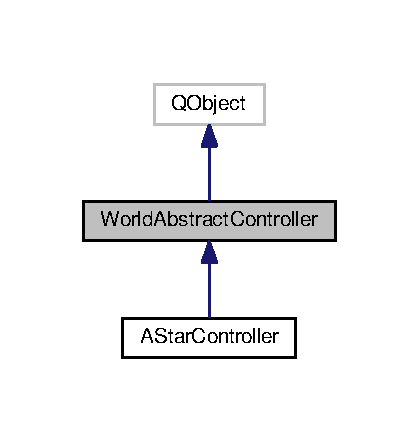
\includegraphics[width=201pt]{d9/d94/classWorldAbstractController__inherit__graph}
\end{center}
\end{figure}


Collaboration diagram for World\+Abstract\+Controller\+:\nopagebreak
\begin{figure}[H]
\begin{center}
\leavevmode
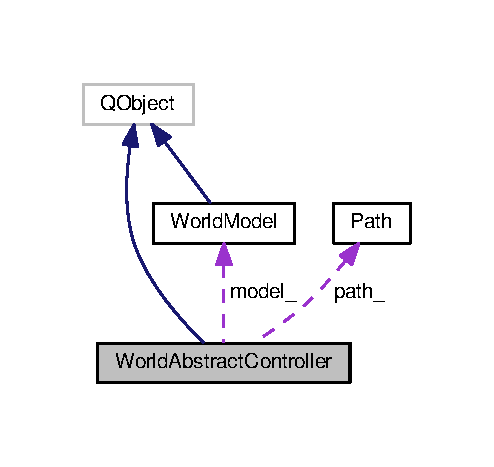
\includegraphics[width=237pt]{d1/d39/classWorldAbstractController__coll__graph}
\end{center}
\end{figure}
\subsection*{Public Slots}
\begin{DoxyCompactItemize}
\item 
virtual void \hyperlink{classWorldAbstractController_af2ab5103153a68f66dcdf75d6c9a4d93}{init} ()=0
\begin{DoxyCompactList}\small\item\em Initialization of the controller. \end{DoxyCompactList}\item 
void \hyperlink{classWorldAbstractController_ab271df7d1af98b87afc0d50a4156616a}{set\+Animation\+Speed} (int value)
\begin{DoxyCompactList}\small\item\em Set animation speed. \end{DoxyCompactList}\end{DoxyCompactItemize}
\subsection*{Signals}
\begin{DoxyCompactItemize}
\item 
void \hyperlink{classWorldAbstractController_ae967946c752a88d3e18a365389f349eb}{animation\+Done} ()
\begin{DoxyCompactList}\small\item\em Animation finished signal. \end{DoxyCompactList}\end{DoxyCompactItemize}
\subsection*{Public Member Functions}
\begin{DoxyCompactItemize}
\item 
\hyperlink{classWorldAbstractController_a8f4be5436078c93733197d76809df45c}{World\+Abstract\+Controller} (\hyperlink{classWorldModel}{World\+Model} $\ast$model)
\begin{DoxyCompactList}\small\item\em Class constructor. \end{DoxyCompactList}\item 
bool \hyperlink{classWorldAbstractController_a6fdee5689b6fd4b2e8f69d26c0181840}{move} (const Q\+Point \&from, const Q\+Point \&to)
\begin{DoxyCompactList}\small\item\em Move protagonist to the position. \end{DoxyCompactList}\item 
Tile $\ast$ \hyperlink{classWorldAbstractController_ac5789c244d880519632c14c073773389}{find\+Closest} (\hyperlink{worldabstractcontroller_8h_a842c5e2e69277690b064bf363c017980}{Object\+Type} type, float min\+Value=0.\+0f, float max\+Value=100.\+0f)
\begin{DoxyCompactList}\small\item\em Find the closest object of a given type. \end{DoxyCompactList}\item 
virtual bool \hyperlink{classWorldAbstractController_a7716b59b6e3cbd086485e7012ae7d4f0}{find\+Path} (const Q\+Point \&from, const Q\+Point \&to, float max\+Cost=I\+N\+F\+I\+N\+I\+TY)=0
\begin{DoxyCompactList}\small\item\em Find the path to the position. \end{DoxyCompactList}\item 
const \hyperlink{structPath}{Path} \& \hyperlink{classWorldAbstractController_ad3c7531df375e1a5b97e0532acb9c28e}{current\+Path} ()\hypertarget{classWorldAbstractController_ad3c7531df375e1a5b97e0532acb9c28e}{}\label{classWorldAbstractController_ad3c7531df375e1a5b97e0532acb9c28e}

\begin{DoxyCompactList}\small\item\em Returns last calculated path. \end{DoxyCompactList}\item 
void \hyperlink{classWorldAbstractController_ad7c83b4de6ee365ef241c0755faa6e0d}{set\+Optimization\+Level} (float value)
\begin{DoxyCompactList}\small\item\em Set level of optimization, e.\+g. h weight in A$\ast$ controller. \end{DoxyCompactList}\item 
virtual void \hyperlink{classWorldAbstractController_a7e70e58d1a22f825034c7d583bf8d662}{set\+Min\+Cost} (float value)
\begin{DoxyCompactList}\small\item\em Set minimal tile energy cost. \end{DoxyCompactList}\item 
void \hyperlink{classWorldAbstractController_a803d78a89d8aa8644e6755d86cb55a5f}{stop} ()\hypertarget{classWorldAbstractController_a803d78a89d8aa8644e6755d86cb55a5f}{}\label{classWorldAbstractController_a803d78a89d8aa8644e6755d86cb55a5f}

\begin{DoxyCompactList}\small\item\em Stop the animation and clear the last path. \end{DoxyCompactList}\end{DoxyCompactItemize}
\subsection*{Protected Member Functions}
\begin{DoxyCompactItemize}
\item 
float \hyperlink{classWorldAbstractController_a556c8e2b55b017f5e837db2b58d3553e}{calculate\+Cost} (float tile)
\begin{DoxyCompactList}\small\item\em Translate tile value to energy cost. \end{DoxyCompactList}\end{DoxyCompactItemize}
\subsection*{Protected Attributes}
\begin{DoxyCompactItemize}
\item 
\hyperlink{classWorldModel}{World\+Model} $\ast$ \hyperlink{classWorldAbstractController_a45fe9595cbcc1eafe6f3f418a08f46c4}{model\+\_\+}\hypertarget{classWorldAbstractController_a45fe9595cbcc1eafe6f3f418a08f46c4}{}\label{classWorldAbstractController_a45fe9595cbcc1eafe6f3f418a08f46c4}

\begin{DoxyCompactList}\small\item\em Owner of the controller. \end{DoxyCompactList}\item 
\hyperlink{structPath}{Path} \hyperlink{classWorldAbstractController_a8e42846e0e46245149339a79758c8a4b}{path\+\_\+}\hypertarget{classWorldAbstractController_a8e42846e0e46245149339a79758c8a4b}{}\label{classWorldAbstractController_a8e42846e0e46245149339a79758c8a4b}

\begin{DoxyCompactList}\small\item\em Last calculated path. \end{DoxyCompactList}\item 
Q\+Timer \hyperlink{classWorldAbstractController_ad152162c39be7f44e48f5ab2de7fcafa}{animation\+\_\+}\hypertarget{classWorldAbstractController_ad152162c39be7f44e48f5ab2de7fcafa}{}\label{classWorldAbstractController_ad152162c39be7f44e48f5ab2de7fcafa}

\begin{DoxyCompactList}\small\item\em Animation timer. \end{DoxyCompactList}\item 
float \hyperlink{classWorldAbstractController_abaf4fb0106d4f5ee475b609a1b3116dd}{optimization\+\_\+}\hypertarget{classWorldAbstractController_abaf4fb0106d4f5ee475b609a1b3116dd}{}\label{classWorldAbstractController_abaf4fb0106d4f5ee475b609a1b3116dd}

\begin{DoxyCompactList}\small\item\em Optimization level. \end{DoxyCompactList}\item 
float \hyperlink{classWorldAbstractController_ad6c2ffd420b9c691d372a8232ab128cc}{min\+Cost\+\_\+} \{0.\+01f\}
\begin{DoxyCompactList}\small\item\em Minimal energy cost of a tile (white tile energy cost) \end{DoxyCompactList}\end{DoxyCompactItemize}


\subsection{Detailed Description}
Abstract controller class. 

Defines the basic functionality of the world model controller. In order to implement a new controller, this class should be inherited, its type should be added to Controller\+Type, init and find\+Path should be re-\/implemented 

\subsection{Constructor \& Destructor Documentation}
\index{World\+Abstract\+Controller@{World\+Abstract\+Controller}!World\+Abstract\+Controller@{World\+Abstract\+Controller}}
\index{World\+Abstract\+Controller@{World\+Abstract\+Controller}!World\+Abstract\+Controller@{World\+Abstract\+Controller}}
\subsubsection[{\texorpdfstring{World\+Abstract\+Controller(\+World\+Model $\ast$model)}{WorldAbstractController(WorldModel *model)}}]{\setlength{\rightskip}{0pt plus 5cm}World\+Abstract\+Controller\+::\+World\+Abstract\+Controller (
\begin{DoxyParamCaption}
\item[{{\bf World\+Model} $\ast$}]{model}
\end{DoxyParamCaption}
)\hspace{0.3cm}{\ttfamily [explicit]}}\hypertarget{classWorldAbstractController_a8f4be5436078c93733197d76809df45c}{}\label{classWorldAbstractController_a8f4be5436078c93733197d76809df45c}


Class constructor. 


\begin{DoxyParams}{Parameters}
{\em model} & owner of the controller \\
\hline
\end{DoxyParams}


\subsection{Member Function Documentation}
\index{World\+Abstract\+Controller@{World\+Abstract\+Controller}!animation\+Done@{animation\+Done}}
\index{animation\+Done@{animation\+Done}!World\+Abstract\+Controller@{World\+Abstract\+Controller}}
\subsubsection[{\texorpdfstring{animation\+Done}{animationDone}}]{\setlength{\rightskip}{0pt plus 5cm}void World\+Abstract\+Controller\+::animation\+Done (
\begin{DoxyParamCaption}
{}
\end{DoxyParamCaption}
)\hspace{0.3cm}{\ttfamily [signal]}}\hypertarget{classWorldAbstractController_ae967946c752a88d3e18a365389f349eb}{}\label{classWorldAbstractController_ae967946c752a88d3e18a365389f349eb}


Animation finished signal. 

Emitted every time the path is performed completely \index{World\+Abstract\+Controller@{World\+Abstract\+Controller}!calculate\+Cost@{calculate\+Cost}}
\index{calculate\+Cost@{calculate\+Cost}!World\+Abstract\+Controller@{World\+Abstract\+Controller}}
\subsubsection[{\texorpdfstring{calculate\+Cost(float tile)}{calculateCost(float tile)}}]{\setlength{\rightskip}{0pt plus 5cm}float World\+Abstract\+Controller\+::calculate\+Cost (
\begin{DoxyParamCaption}
\item[{float}]{tile}
\end{DoxyParamCaption}
)\hspace{0.3cm}{\ttfamily [inline]}, {\ttfamily [protected]}}\hypertarget{classWorldAbstractController_a556c8e2b55b017f5e837db2b58d3553e}{}\label{classWorldAbstractController_a556c8e2b55b017f5e837db2b58d3553e}


Translate tile value to energy cost. 


\begin{DoxyParams}{Parameters}
{\em tile} & tile value \\
\hline
\end{DoxyParams}
\begin{DoxyReturn}{Returns}
energy cost 
\end{DoxyReturn}
\index{World\+Abstract\+Controller@{World\+Abstract\+Controller}!find\+Closest@{find\+Closest}}
\index{find\+Closest@{find\+Closest}!World\+Abstract\+Controller@{World\+Abstract\+Controller}}
\subsubsection[{\texorpdfstring{find\+Closest(\+Object\+Type type, float min\+Value=0.\+0f, float max\+Value=100.\+0f)}{findClosest(ObjectType type, float minValue=0.0f, float maxValue=100.0f)}}]{\setlength{\rightskip}{0pt plus 5cm}Tile $\ast$ World\+Abstract\+Controller\+::find\+Closest (
\begin{DoxyParamCaption}
\item[{{\bf Object\+Type}}]{type, }
\item[{float}]{min\+Value = {\ttfamily 0.0f}, }
\item[{float}]{max\+Value = {\ttfamily 100.0f}}
\end{DoxyParamCaption}
)}\hypertarget{classWorldAbstractController_ac5789c244d880519632c14c073773389}{}\label{classWorldAbstractController_ac5789c244d880519632c14c073773389}


Find the closest object of a given type. 

Searches for the closest object, enemy or health pack, with a given max and min values.


\begin{DoxyParams}{Parameters}
{\em type} & type of object \\
\hline
{\em min\+Value} & minimal tile value(strength of the enemy or H\+P of health pack) \\
\hline
{\em max\+Value} & maximal tile value(strength of the enemy or H\+P of health pack) \\
\hline
\end{DoxyParams}
\begin{DoxyReturn}{Returns}
Tile pointer to the object. If no object was found, returns nullptr
\end{DoxyReturn}
\begin{DoxySeeAlso}{See also}
\hyperlink{worldabstractcontroller_8h_a842c5e2e69277690b064bf363c017980}{Object\+Type} 
\end{DoxySeeAlso}
\index{World\+Abstract\+Controller@{World\+Abstract\+Controller}!find\+Path@{find\+Path}}
\index{find\+Path@{find\+Path}!World\+Abstract\+Controller@{World\+Abstract\+Controller}}
\subsubsection[{\texorpdfstring{find\+Path(const Q\+Point \&from, const Q\+Point \&to, float max\+Cost=\+I\+N\+F\+I\+N\+I\+T\+Y)=0}{findPath(const QPoint &from, const QPoint &to, float maxCost=INFINITY)=0}}]{\setlength{\rightskip}{0pt plus 5cm}virtual bool World\+Abstract\+Controller\+::find\+Path (
\begin{DoxyParamCaption}
\item[{const Q\+Point \&}]{from, }
\item[{const Q\+Point \&}]{to, }
\item[{float}]{max\+Cost = {\ttfamily INFINITY}}
\end{DoxyParamCaption}
)\hspace{0.3cm}{\ttfamily [pure virtual]}}\hypertarget{classWorldAbstractController_a7716b59b6e3cbd086485e7012ae7d4f0}{}\label{classWorldAbstractController_a7716b59b6e3cbd086485e7012ae7d4f0}


Find the path to the position. 

\begin{DoxyNote}{Note}
This is a virtual function to be implemented by successors 
\end{DoxyNote}

\begin{DoxyParams}{Parameters}
{\em from} & starting point \\
\hline
{\em to} & destination \\
\hline
\end{DoxyParams}
\begin{DoxyReturn}{Returns}
true if the path was find, false otherwise 
\end{DoxyReturn}


Implemented in \hyperlink{classAStarController_aa230f8e80731d01daa502af943fe350e}{A\+Star\+Controller}.

\index{World\+Abstract\+Controller@{World\+Abstract\+Controller}!init@{init}}
\index{init@{init}!World\+Abstract\+Controller@{World\+Abstract\+Controller}}
\subsubsection[{\texorpdfstring{init}{init}}]{\setlength{\rightskip}{0pt plus 5cm}virtual void World\+Abstract\+Controller\+::init (
\begin{DoxyParamCaption}
{}
\end{DoxyParamCaption}
)\hspace{0.3cm}{\ttfamily [pure virtual]}, {\ttfamily [slot]}}\hypertarget{classWorldAbstractController_af2ab5103153a68f66dcdf75d6c9a4d93}{}\label{classWorldAbstractController_af2ab5103153a68f66dcdf75d6c9a4d93}


Initialization of the controller. 

\begin{DoxyNote}{Note}
This is a virtual function to be implemented by successors 
\end{DoxyNote}


Implemented in \hyperlink{classAStarController_a228a9bd549dbae704ed6663ed726053e}{A\+Star\+Controller}.

\index{World\+Abstract\+Controller@{World\+Abstract\+Controller}!move@{move}}
\index{move@{move}!World\+Abstract\+Controller@{World\+Abstract\+Controller}}
\subsubsection[{\texorpdfstring{move(const Q\+Point \&from, const Q\+Point \&to)}{move(const QPoint &from, const QPoint &to)}}]{\setlength{\rightskip}{0pt plus 5cm}bool World\+Abstract\+Controller\+::move (
\begin{DoxyParamCaption}
\item[{const Q\+Point \&}]{from, }
\item[{const Q\+Point \&}]{to}
\end{DoxyParamCaption}
)}\hypertarget{classWorldAbstractController_a6fdee5689b6fd4b2e8f69d26c0181840}{}\label{classWorldAbstractController_a6fdee5689b6fd4b2e8f69d26c0181840}


Move protagonist to the position. 

Finds the path to a given point and animates the movement to it 
\begin{DoxyParams}{Parameters}
{\em from} & starting point \\
\hline
{\em to} & destination \\
\hline
\end{DoxyParams}
\index{World\+Abstract\+Controller@{World\+Abstract\+Controller}!set\+Animation\+Speed@{set\+Animation\+Speed}}
\index{set\+Animation\+Speed@{set\+Animation\+Speed}!World\+Abstract\+Controller@{World\+Abstract\+Controller}}
\subsubsection[{\texorpdfstring{set\+Animation\+Speed}{setAnimationSpeed}}]{\setlength{\rightskip}{0pt plus 5cm}void World\+Abstract\+Controller\+::set\+Animation\+Speed (
\begin{DoxyParamCaption}
\item[{int}]{value}
\end{DoxyParamCaption}
)\hspace{0.3cm}{\ttfamily [slot]}}\hypertarget{classWorldAbstractController_ab271df7d1af98b87afc0d50a4156616a}{}\label{classWorldAbstractController_ab271df7d1af98b87afc0d50a4156616a}


Set animation speed. 

Set animation speed between 100(fastest) and 1(slowest) 
\begin{DoxyParams}{Parameters}
{\em value} & animation speed \\
\hline
\end{DoxyParams}
\index{World\+Abstract\+Controller@{World\+Abstract\+Controller}!set\+Min\+Cost@{set\+Min\+Cost}}
\index{set\+Min\+Cost@{set\+Min\+Cost}!World\+Abstract\+Controller@{World\+Abstract\+Controller}}
\subsubsection[{\texorpdfstring{set\+Min\+Cost(float value)}{setMinCost(float value)}}]{\setlength{\rightskip}{0pt plus 5cm}void World\+Abstract\+Controller\+::set\+Min\+Cost (
\begin{DoxyParamCaption}
\item[{float}]{value}
\end{DoxyParamCaption}
)\hspace{0.3cm}{\ttfamily [virtual]}}\hypertarget{classWorldAbstractController_a7e70e58d1a22f825034c7d583bf8d662}{}\label{classWorldAbstractController_a7e70e58d1a22f825034c7d583bf8d662}


Set minimal tile energy cost. 

Defines the energy cost of white tile 
\begin{DoxyParams}{Parameters}
{\em value} & energy cost multiplied by 1000 \\
\hline
\end{DoxyParams}
\index{World\+Abstract\+Controller@{World\+Abstract\+Controller}!set\+Optimization\+Level@{set\+Optimization\+Level}}
\index{set\+Optimization\+Level@{set\+Optimization\+Level}!World\+Abstract\+Controller@{World\+Abstract\+Controller}}
\subsubsection[{\texorpdfstring{set\+Optimization\+Level(float value)}{setOptimizationLevel(float value)}}]{\setlength{\rightskip}{0pt plus 5cm}void World\+Abstract\+Controller\+::set\+Optimization\+Level (
\begin{DoxyParamCaption}
\item[{float}]{value}
\end{DoxyParamCaption}
)\hspace{0.3cm}{\ttfamily [inline]}}\hypertarget{classWorldAbstractController_ad7c83b4de6ee365ef241c0755faa6e0d}{}\label{classWorldAbstractController_ad7c83b4de6ee365ef241c0755faa6e0d}


Set level of optimization, e.\+g. h weight in A$\ast$ controller. 


\begin{DoxyParams}{Parameters}
{\em value} & level from 0 to 100 \\
\hline
\end{DoxyParams}


\subsection{Member Data Documentation}
\index{World\+Abstract\+Controller@{World\+Abstract\+Controller}!min\+Cost\+\_\+@{min\+Cost\+\_\+}}
\index{min\+Cost\+\_\+@{min\+Cost\+\_\+}!World\+Abstract\+Controller@{World\+Abstract\+Controller}}
\subsubsection[{\texorpdfstring{min\+Cost\+\_\+}{minCost_}}]{\setlength{\rightskip}{0pt plus 5cm}float World\+Abstract\+Controller\+::min\+Cost\+\_\+ \{0.\+01f\}\hspace{0.3cm}{\ttfamily [protected]}}\hypertarget{classWorldAbstractController_ad6c2ffd420b9c691d372a8232ab128cc}{}\label{classWorldAbstractController_ad6c2ffd420b9c691d372a8232ab128cc}


Minimal energy cost of a tile (white tile energy cost) 

\begin{DoxySeeAlso}{See also}
\hyperlink{classWorldAbstractController_a556c8e2b55b017f5e837db2b58d3553e}{calculate\+Cost} 
\end{DoxySeeAlso}


The documentation for this class was generated from the following files\+:\begin{DoxyCompactItemize}
\item 
/home/bobiko/ku-\/leuven/media-\/processing/labs/finaltask/finaltask/src/controller/\hyperlink{worldabstractcontroller_8h}{worldabstractcontroller.\+h}\item 
/home/bobiko/ku-\/leuven/media-\/processing/labs/finaltask/finaltask/src/controller/\hyperlink{worldabstractcontroller_8cpp}{worldabstractcontroller.\+cpp}\end{DoxyCompactItemize}

\hypertarget{classWorldControllerFactory}{}\section{World\+Controller\+Factory Class Reference}
\label{classWorldControllerFactory}\index{World\+Controller\+Factory@{World\+Controller\+Factory}}


Controller factory class.  




{\ttfamily \#include $<$worldcontrollerfactory.\+h$>$}

\subsection*{Static Public Member Functions}
\begin{DoxyCompactItemize}
\item 
static \hyperlink{classWorldAbstractController}{World\+Abstract\+Controller} $\ast$ \hyperlink{classWorldControllerFactory_a90d9c0f2d0b6a58b2ad4336e539057d0}{create\+Controller} (\hyperlink{classWorldModel}{World\+Model} $\ast$model, \hyperlink{group__controller_ga81059b4122c9dd4608d347eb117ae8c9}{Controller\+Type} type=A\+Star)
\begin{DoxyCompactList}\small\item\em Create a controller for the model. \end{DoxyCompactList}\end{DoxyCompactItemize}


\subsection{Detailed Description}
Controller factory class. 

This class is an implementation of factory pattern. Factory is needed since different algorythms can be used for path finding, thus it is sufficient to have a unified interface, in this case \hyperlink{classWorldAbstractController}{World\+Abstract\+Controller} 

\subsection{Member Function Documentation}
\index{World\+Controller\+Factory@{World\+Controller\+Factory}!create\+Controller@{create\+Controller}}
\index{create\+Controller@{create\+Controller}!World\+Controller\+Factory@{World\+Controller\+Factory}}
\subsubsection[{\texorpdfstring{create\+Controller(\+World\+Model $\ast$model, Controller\+Type type=\+A\+Star)}{createController(WorldModel *model, ControllerType type=AStar)}}]{\setlength{\rightskip}{0pt plus 5cm}{\bf World\+Abstract\+Controller} $\ast$ World\+Controller\+Factory\+::create\+Controller (
\begin{DoxyParamCaption}
\item[{{\bf World\+Model} $\ast$}]{model, }
\item[{{\bf Controller\+Type}}]{type = {\ttfamily AStar}}
\end{DoxyParamCaption}
)\hspace{0.3cm}{\ttfamily [static]}}\hypertarget{classWorldControllerFactory_a90d9c0f2d0b6a58b2ad4336e539057d0}{}\label{classWorldControllerFactory_a90d9c0f2d0b6a58b2ad4336e539057d0}


Create a controller for the model. 


\begin{DoxyParams}{Parameters}
{\em model} & pointer to owner of the controller \\
\hline
{\em type} & type of controller \\
\hline
\end{DoxyParams}
\begin{DoxyReturn}{Returns}
created controller 
\end{DoxyReturn}


The documentation for this class was generated from the following files\+:\begin{DoxyCompactItemize}
\item 
/home/bobiko/ku-\/leuven/media-\/processing/labs/finaltask/finaltask/src/controller/\hyperlink{worldcontrollerfactory_8h}{worldcontrollerfactory.\+h}\item 
/home/bobiko/ku-\/leuven/media-\/processing/labs/finaltask/finaltask/src/controller/\hyperlink{worldcontrollerfactory_8cpp}{worldcontrollerfactory.\+cpp}\end{DoxyCompactItemize}

\hypertarget{classWorldGraphicsView}{}\section{World\+Graphics\+View Class Reference}
\label{classWorldGraphicsView}\index{World\+Graphics\+View@{World\+Graphics\+View}}


Graphics view component class implementation.  




{\ttfamily \#include $<$worldgraphicsview.\+h$>$}



Inheritance diagram for World\+Graphics\+View\+:\nopagebreak
\begin{figure}[H]
\begin{center}
\leavevmode
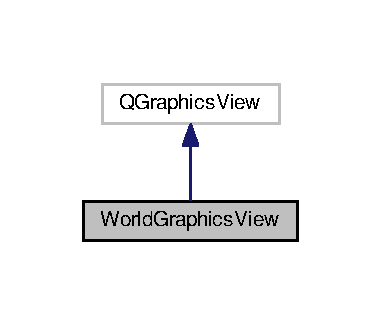
\includegraphics[width=183pt]{d8/d05/classWorldGraphicsView__inherit__graph}
\end{center}
\end{figure}


Collaboration diagram for World\+Graphics\+View\+:\nopagebreak
\begin{figure}[H]
\begin{center}
\leavevmode
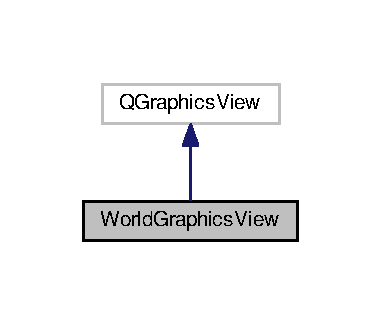
\includegraphics[width=183pt]{d9/d69/classWorldGraphicsView__coll__graph}
\end{center}
\end{figure}
\subsection*{Public Slots}
\begin{DoxyCompactItemize}
\item 
void \hyperlink{classWorldGraphicsView_afe30c74f794ae1b385ca3a89cb9ede25}{on\+Protagonist\+Position\+Changed} (int x, int y)
\begin{DoxyCompactList}\small\item\em Update protagonist position. \end{DoxyCompactList}\item 
void \hyperlink{classWorldGraphicsView_a8bdead6606060dc49a5faa5464d94c8d}{reload\+Scene} ()
\begin{DoxyCompactList}\small\item\em Reload the model slot. \end{DoxyCompactList}\item 
void \hyperlink{classWorldGraphicsView_a57c88f9c11bd3bc2df3aeba015d8ca67}{enlarge} ()\hypertarget{classWorldGraphicsView_a57c88f9c11bd3bc2df3aeba015d8ca67}{}\label{classWorldGraphicsView_a57c88f9c11bd3bc2df3aeba015d8ca67}

\begin{DoxyCompactList}\small\item\em Scale the scene up. \end{DoxyCompactList}\item 
void \hyperlink{classWorldGraphicsView_a87a8d6055562a76d6e7e3b61832497cf}{shrink} ()\hypertarget{classWorldGraphicsView_a87a8d6055562a76d6e7e3b61832497cf}{}\label{classWorldGraphicsView_a87a8d6055562a76d6e7e3b61832497cf}

\begin{DoxyCompactList}\small\item\em Scale the scene down. \end{DoxyCompactList}\end{DoxyCompactItemize}
\subsection*{Public Member Functions}
\begin{DoxyCompactItemize}
\item 
\hyperlink{classWorldGraphicsView_aac181c5fb59c553a885afc62c9f58576}{World\+Graphics\+View} (Q\+Widget $\ast$parent=0)
\begin{DoxyCompactList}\small\item\em Class constructor. \end{DoxyCompactList}\item 
void \hyperlink{classWorldGraphicsView_ac9bfe6153b0106f0cb6591b511f9391a}{set\+Model} (\hyperlink{classWorldModel}{World\+Model} $\ast$model)
\begin{DoxyCompactList}\small\item\em Set the data model. \end{DoxyCompactList}\item 
virtual void \hyperlink{classWorldGraphicsView_abdb212ddc141fdc73054bab7b5320d51}{key\+Press\+Event} (Q\+Key\+Event $\ast$e) override
\begin{DoxyCompactList}\small\item\em Key press event handler. \end{DoxyCompactList}\item 
virtual void \hyperlink{classWorldGraphicsView_af4b8a71cfd9f363c8056a506ef60344c}{mouse\+Press\+Event} (Q\+Mouse\+Event $\ast$e) override
\begin{DoxyCompactList}\small\item\em Mouse press event handler. \end{DoxyCompactList}\item 
virtual void \hyperlink{classWorldGraphicsView_a07a8843b73603a3eb71f768308aa5310}{mouse\+Move\+Event} (Q\+Mouse\+Event $\ast$e) override
\begin{DoxyCompactList}\small\item\em Mouse move event handler. \end{DoxyCompactList}\end{DoxyCompactItemize}


\subsection{Detailed Description}
Graphics view component class implementation. 

The class is based on Q\+Graphics\+View and uses Q\+Graphics\+Scene as a graphical model(scene), and a \hyperlink{classWorldModel}{World\+Model} instance as a data model for the scene. 

\subsection{Constructor \& Destructor Documentation}
\index{World\+Graphics\+View@{World\+Graphics\+View}!World\+Graphics\+View@{World\+Graphics\+View}}
\index{World\+Graphics\+View@{World\+Graphics\+View}!World\+Graphics\+View@{World\+Graphics\+View}}
\subsubsection[{\texorpdfstring{World\+Graphics\+View(\+Q\+Widget $\ast$parent=0)}{WorldGraphicsView(QWidget *parent=0)}}]{\setlength{\rightskip}{0pt plus 5cm}World\+Graphics\+View\+::\+World\+Graphics\+View (
\begin{DoxyParamCaption}
\item[{Q\+Widget $\ast$}]{parent = {\ttfamily 0}}
\end{DoxyParamCaption}
)}\hypertarget{classWorldGraphicsView_aac181c5fb59c553a885afc62c9f58576}{}\label{classWorldGraphicsView_aac181c5fb59c553a885afc62c9f58576}


Class constructor. 


\begin{DoxyParams}{Parameters}
{\em parent} & visual parent of the view \\
\hline
\end{DoxyParams}


\subsection{Member Function Documentation}
\index{World\+Graphics\+View@{World\+Graphics\+View}!key\+Press\+Event@{key\+Press\+Event}}
\index{key\+Press\+Event@{key\+Press\+Event}!World\+Graphics\+View@{World\+Graphics\+View}}
\subsubsection[{\texorpdfstring{key\+Press\+Event(\+Q\+Key\+Event $\ast$e) override}{keyPressEvent(QKeyEvent *e) override}}]{\setlength{\rightskip}{0pt plus 5cm}void World\+Graphics\+View\+::key\+Press\+Event (
\begin{DoxyParamCaption}
\item[{Q\+Key\+Event $\ast$}]{e}
\end{DoxyParamCaption}
)\hspace{0.3cm}{\ttfamily [override]}, {\ttfamily [virtual]}}\hypertarget{classWorldGraphicsView_abdb212ddc141fdc73054bab7b5320d51}{}\label{classWorldGraphicsView_abdb212ddc141fdc73054bab7b5320d51}


Key press event handler. 


\begin{DoxyParams}{Parameters}
{\em e} & key event \\
\hline
\end{DoxyParams}
\index{World\+Graphics\+View@{World\+Graphics\+View}!mouse\+Move\+Event@{mouse\+Move\+Event}}
\index{mouse\+Move\+Event@{mouse\+Move\+Event}!World\+Graphics\+View@{World\+Graphics\+View}}
\subsubsection[{\texorpdfstring{mouse\+Move\+Event(\+Q\+Mouse\+Event $\ast$e) override}{mouseMoveEvent(QMouseEvent *e) override}}]{\setlength{\rightskip}{0pt plus 5cm}void World\+Graphics\+View\+::mouse\+Move\+Event (
\begin{DoxyParamCaption}
\item[{Q\+Mouse\+Event $\ast$}]{e}
\end{DoxyParamCaption}
)\hspace{0.3cm}{\ttfamily [override]}, {\ttfamily [virtual]}}\hypertarget{classWorldGraphicsView_a07a8843b73603a3eb71f768308aa5310}{}\label{classWorldGraphicsView_a07a8843b73603a3eb71f768308aa5310}


Mouse move event handler. 


\begin{DoxyParams}{Parameters}
{\em e} & mouse event \\
\hline
\end{DoxyParams}
\index{World\+Graphics\+View@{World\+Graphics\+View}!mouse\+Press\+Event@{mouse\+Press\+Event}}
\index{mouse\+Press\+Event@{mouse\+Press\+Event}!World\+Graphics\+View@{World\+Graphics\+View}}
\subsubsection[{\texorpdfstring{mouse\+Press\+Event(\+Q\+Mouse\+Event $\ast$e) override}{mousePressEvent(QMouseEvent *e) override}}]{\setlength{\rightskip}{0pt plus 5cm}void World\+Graphics\+View\+::mouse\+Press\+Event (
\begin{DoxyParamCaption}
\item[{Q\+Mouse\+Event $\ast$}]{e}
\end{DoxyParamCaption}
)\hspace{0.3cm}{\ttfamily [override]}, {\ttfamily [virtual]}}\hypertarget{classWorldGraphicsView_af4b8a71cfd9f363c8056a506ef60344c}{}\label{classWorldGraphicsView_af4b8a71cfd9f363c8056a506ef60344c}


Mouse press event handler. 


\begin{DoxyParams}{Parameters}
{\em e} & mouse event \\
\hline
\end{DoxyParams}
\index{World\+Graphics\+View@{World\+Graphics\+View}!on\+Protagonist\+Position\+Changed@{on\+Protagonist\+Position\+Changed}}
\index{on\+Protagonist\+Position\+Changed@{on\+Protagonist\+Position\+Changed}!World\+Graphics\+View@{World\+Graphics\+View}}
\subsubsection[{\texorpdfstring{on\+Protagonist\+Position\+Changed}{onProtagonistPositionChanged}}]{\setlength{\rightskip}{0pt plus 5cm}void World\+Graphics\+View\+::on\+Protagonist\+Position\+Changed (
\begin{DoxyParamCaption}
\item[{int}]{x, }
\item[{int}]{y}
\end{DoxyParamCaption}
)\hspace{0.3cm}{\ttfamily [slot]}}\hypertarget{classWorldGraphicsView_afe30c74f794ae1b385ca3a89cb9ede25}{}\label{classWorldGraphicsView_afe30c74f794ae1b385ca3a89cb9ede25}


Update protagonist position. 

Move protagonist item to a given point and centers the view on this position 
\begin{DoxyParams}{Parameters}
{\em x} & horizontal coordinate \\
\hline
{\em y} & vertical coordinate \\
\hline
\end{DoxyParams}
\index{World\+Graphics\+View@{World\+Graphics\+View}!reload\+Scene@{reload\+Scene}}
\index{reload\+Scene@{reload\+Scene}!World\+Graphics\+View@{World\+Graphics\+View}}
\subsubsection[{\texorpdfstring{reload\+Scene}{reloadScene}}]{\setlength{\rightskip}{0pt plus 5cm}void World\+Graphics\+View\+::reload\+Scene (
\begin{DoxyParamCaption}
{}
\end{DoxyParamCaption}
)\hspace{0.3cm}{\ttfamily [slot]}}\hypertarget{classWorldGraphicsView_a8bdead6606060dc49a5faa5464d94c8d}{}\label{classWorldGraphicsView_a8bdead6606060dc49a5faa5464d94c8d}


Reload the model slot. 

Re-\/initializes the scene in accordance with a given model. \index{World\+Graphics\+View@{World\+Graphics\+View}!set\+Model@{set\+Model}}
\index{set\+Model@{set\+Model}!World\+Graphics\+View@{World\+Graphics\+View}}
\subsubsection[{\texorpdfstring{set\+Model(\+World\+Model $\ast$model)}{setModel(WorldModel *model)}}]{\setlength{\rightskip}{0pt plus 5cm}void World\+Graphics\+View\+::set\+Model (
\begin{DoxyParamCaption}
\item[{{\bf World\+Model} $\ast$}]{model}
\end{DoxyParamCaption}
)}\hypertarget{classWorldGraphicsView_ac9bfe6153b0106f0cb6591b511f9391a}{}\label{classWorldGraphicsView_ac9bfe6153b0106f0cb6591b511f9391a}


Set the data model. 

Every time a new model is set, the view re-\/initializes the scene in accordance with a given model.


\begin{DoxyParams}{Parameters}
{\em model} & model to be set \\
\hline
\end{DoxyParams}


The documentation for this class was generated from the following files\+:\begin{DoxyCompactItemize}
\item 
/home/bobiko/ku-\/leuven/media-\/processing/labs/finaltask/finaltask/src/graphicsview/\hyperlink{worldgraphicsview_8h}{worldgraphicsview.\+h}\item 
/home/bobiko/ku-\/leuven/media-\/processing/labs/finaltask/finaltask/src/graphicsview/\hyperlink{worldgraphicsview_8cpp}{worldgraphicsview.\+cpp}\end{DoxyCompactItemize}

\hypertarget{classWorldModel}{}\section{World\+Model Class Reference}
\label{classWorldModel}\index{World\+Model@{World\+Model}}


Model component implementation.  




{\ttfamily \#include $<$worldmodel.\+h$>$}



Inheritance diagram for World\+Model\+:\nopagebreak
\begin{figure}[H]
\begin{center}
\leavevmode
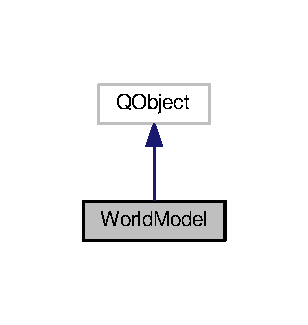
\includegraphics[width=148pt]{de/d4d/classWorldModel__inherit__graph}
\end{center}
\end{figure}


Collaboration diagram for World\+Model\+:\nopagebreak
\begin{figure}[H]
\begin{center}
\leavevmode
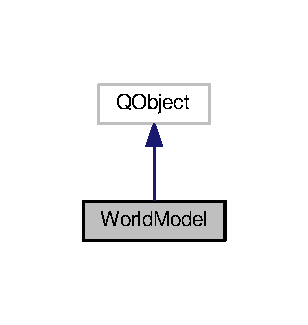
\includegraphics[width=148pt]{da/dcc/classWorldModel__coll__graph}
\end{center}
\end{figure}
\subsection*{Public Slots}
\begin{DoxyCompactItemize}
\item 
void \hyperlink{classWorldModel_ae0cc05dba8df542709d08ece9d3412db}{attack\+Enemy} ()
\begin{DoxyCompactList}\small\item\em Attack an enemy at the position. \end{DoxyCompactList}\item 
void \hyperlink{classWorldModel_a8cb4ca5355bd9825deefbf8cc86f067a}{use\+Healthpack} ()
\begin{DoxyCompactList}\small\item\em Use a health pack at the position. \end{DoxyCompactList}\item 
void \hyperlink{classWorldModel_a68cdcbf4857f21bf0af3042d7a73cdc4}{poison\+Area} (int value, Q\+Rect rect)
\begin{DoxyCompactList}\small\item\em Spead the poison slot. \end{DoxyCompactList}\item 
void \hyperlink{classWorldModel_ae02716d99230f6edb0f7caf5b469bc1c}{move} (int x, int y)
\begin{DoxyCompactList}\small\item\em Move the protagonist to a certain position. \end{DoxyCompactList}\item 
void \hyperlink{classWorldModel_add90c164136141295e968e9419b3f3a9}{move} (const Q\+Point \&pos)
\begin{DoxyCompactList}\small\item\em Move the protagonist to a certain position. \end{DoxyCompactList}\end{DoxyCompactItemize}
\subsection*{Signals}
\begin{DoxyCompactItemize}
\item 
void \hyperlink{classWorldModel_a9ee97272fc756d45c411f578f98905af}{reload} ()\hypertarget{classWorldModel_a9ee97272fc756d45c411f578f98905af}{}\label{classWorldModel_a9ee97272fc756d45c411f578f98905af}

\begin{DoxyCompactList}\small\item\em Reload signal Emited every time \hyperlink{classWorldModel_a9003814b10d3b533d3c4313613712493}{init()} is called. \end{DoxyCompactList}\item 
void \hyperlink{classWorldModel_a1f403da0540ae3e4fe55ea7262ee2fe8}{healthpack\+Used} (int x, int y)
\begin{DoxyCompactList}\small\item\em Health pack is used signal Emited every time one of health packs is used. \end{DoxyCompactList}\item 
void \hyperlink{classWorldModel_af66c7d6051c21a0933e9ac168096dd8b}{enemy\+Defeated} (int x, int y)
\begin{DoxyCompactList}\small\item\em Enemy is defeated signal Emited every time one of enemies is defeated. \end{DoxyCompactList}\item 
void \hyperlink{classWorldModel_aceb49c5514940947dbcacc97484aa4bd}{area\+Poisoned} (int value, Q\+Rect rect)
\begin{DoxyCompactList}\small\item\em Area is poisoned signal. \end{DoxyCompactList}\item 
void \hyperlink{classWorldModel_a128eb886de920133792e1e26f1caf468}{win} ()
\begin{DoxyCompactList}\small\item\em Win signal. \end{DoxyCompactList}\item 
void \hyperlink{classWorldModel_a73bdac0d024fd7ae02f09b58e833cad3}{protagonist\+Dead} ()
\begin{DoxyCompactList}\small\item\em Protagonist is dead signal. \end{DoxyCompactList}\item 
void \hyperlink{classWorldModel_ad97bbf59d3714296882d2be9038e27bb}{protagonist\+No\+Energy} ()
\begin{DoxyCompactList}\small\item\em Protagonist ran out of energy signal. \end{DoxyCompactList}\end{DoxyCompactItemize}
\subsection*{Public Member Functions}
\begin{DoxyCompactItemize}
\item 
\hyperlink{classWorldModel_a6787b97a5c8826279e9a31740819f277}{World\+Model} (Q\+Object $\ast$parent=0)
\begin{DoxyCompactList}\small\item\em Class constructor. \end{DoxyCompactList}\item 
void \hyperlink{classWorldModel_a9003814b10d3b533d3c4313613712493}{init} (Q\+String filename=\char`\"{}\char`\"{}, int enemies=0, int healthpacks=0)
\begin{DoxyCompactList}\small\item\em Initialization of the model. \end{DoxyCompactList}\item 
const std\+::unique\+\_\+ptr$<$ \hyperlink{classUWorld}{U\+World} $>$ \& \hyperlink{classWorldModel_a0b50ae0247e6c6553ab39f47e4dd54ca}{get\+World} () const \hypertarget{classWorldModel_a0b50ae0247e6c6553ab39f47e4dd54ca}{}\label{classWorldModel_a0b50ae0247e6c6553ab39f47e4dd54ca}

\begin{DoxyCompactList}\small\item\em Return World instance of the model. \end{DoxyCompactList}\item 
const std\+::vector$<$ std\+::unique\+\_\+ptr$<$ \hyperlink{classUEnemy}{U\+Enemy} $>$ $>$ \& \hyperlink{classWorldModel_ad14d1117ade3ef9fbc16c0384c505e82}{get\+Enemies} () const \hypertarget{classWorldModel_ad14d1117ade3ef9fbc16c0384c505e82}{}\label{classWorldModel_ad14d1117ade3ef9fbc16c0384c505e82}

\begin{DoxyCompactList}\small\item\em Returns vector of unique pointers to regular enemies. \end{DoxyCompactList}\item 
const std\+::vector$<$ std\+::unique\+\_\+ptr$<$ \hyperlink{classUPEnemy}{U\+P\+Enemy} $>$ $>$ \& \hyperlink{classWorldModel_a3a573fb0a631baa1b7eb788748181bb7}{get\+P\+Enemies} () const \hypertarget{classWorldModel_a3a573fb0a631baa1b7eb788748181bb7}{}\label{classWorldModel_a3a573fb0a631baa1b7eb788748181bb7}

\begin{DoxyCompactList}\small\item\em Returns vector of unique pointers to poisoned enemies. \end{DoxyCompactList}\item 
const std\+::vector$<$ std\+::unique\+\_\+ptr$<$ \hyperlink{classUHealthPack}{U\+Health\+Pack} $>$ $>$ \& \hyperlink{classWorldModel_a81a07a89bb6f67371553656b1780f54d}{get\+Healthpacks} () const \hypertarget{classWorldModel_a81a07a89bb6f67371553656b1780f54d}{}\label{classWorldModel_a81a07a89bb6f67371553656b1780f54d}

\begin{DoxyCompactList}\small\item\em Returns vector of unique pointers to health packs. \end{DoxyCompactList}\item 
const std\+::unique\+\_\+ptr$<$ \hyperlink{classUProtagonist}{U\+Protagonist} $>$ \& \hyperlink{classWorldModel_ae77f38af10f91c3ce963633530f0644a}{get\+Protagonist} () const \hypertarget{classWorldModel_ae77f38af10f91c3ce963633530f0644a}{}\label{classWorldModel_ae77f38af10f91c3ce963633530f0644a}

\begin{DoxyCompactList}\small\item\em Returns unique pointer to protagonist. \end{DoxyCompactList}\item 
const std\+::unique\+\_\+ptr$<$ \hyperlink{classWorldAbstractController}{World\+Abstract\+Controller} $>$ \& \hyperlink{classWorldModel_a7cf1b1a42990ab40ccd638ae868f5f21}{get\+Controller} () const \hypertarget{classWorldModel_a7cf1b1a42990ab40ccd638ae868f5f21}{}\label{classWorldModel_a7cf1b1a42990ab40ccd638ae868f5f21}

\begin{DoxyCompactList}\small\item\em Returns unique pointer to controller. \end{DoxyCompactList}\item 
const Q\+String \& \hyperlink{classWorldModel_a1f4957f65c7b044dffe4d4c5e6886438}{get\+Level} () const \hypertarget{classWorldModel_a1f4957f65c7b044dffe4d4c5e6886438}{}\label{classWorldModel_a1f4957f65c7b044dffe4d4c5e6886438}

\begin{DoxyCompactList}\small\item\em Returns level map image. \end{DoxyCompactList}\item 
bool \hyperlink{classWorldModel_a1ccf488139cdbfa6a25262d01a0401d5}{ready} () const \hypertarget{classWorldModel_a1ccf488139cdbfa6a25262d01a0401d5}{}\label{classWorldModel_a1ccf488139cdbfa6a25262d01a0401d5}

\begin{DoxyCompactList}\small\item\em Check if the model is initialized. \end{DoxyCompactList}\item 
void \hyperlink{classWorldModel_a83284690f9b21540528cf13d114a6dc9}{check\+If\+Win} ()\hypertarget{classWorldModel_a83284690f9b21540528cf13d114a6dc9}{}\label{classWorldModel_a83284690f9b21540528cf13d114a6dc9}

\begin{DoxyCompactList}\small\item\em Check if all enemies are dead. \end{DoxyCompactList}\end{DoxyCompactItemize}


\subsection{Detailed Description}
Model component implementation. 

Stores all the objects created in the world and enables their interactions. 

\subsection{Constructor \& Destructor Documentation}
\index{World\+Model@{World\+Model}!World\+Model@{World\+Model}}
\index{World\+Model@{World\+Model}!World\+Model@{World\+Model}}
\subsubsection[{\texorpdfstring{World\+Model(\+Q\+Object $\ast$parent=0)}{WorldModel(QObject *parent=0)}}]{\setlength{\rightskip}{0pt plus 5cm}World\+Model\+::\+World\+Model (
\begin{DoxyParamCaption}
\item[{Q\+Object $\ast$}]{parent = {\ttfamily 0}}
\end{DoxyParamCaption}
)\hspace{0.3cm}{\ttfamily [explicit]}}\hypertarget{classWorldModel_a6787b97a5c8826279e9a31740819f277}{}\label{classWorldModel_a6787b97a5c8826279e9a31740819f277}


Class constructor. 


\begin{DoxyParams}{Parameters}
{\em parent} & parent object, passed to Q\+Object constructor \\
\hline
\end{DoxyParams}


\subsection{Member Function Documentation}
\index{World\+Model@{World\+Model}!area\+Poisoned@{area\+Poisoned}}
\index{area\+Poisoned@{area\+Poisoned}!World\+Model@{World\+Model}}
\subsubsection[{\texorpdfstring{area\+Poisoned}{areaPoisoned}}]{\setlength{\rightskip}{0pt plus 5cm}void World\+Model\+::area\+Poisoned (
\begin{DoxyParamCaption}
\item[{int}]{value, }
\item[{Q\+Rect}]{rect}
\end{DoxyParamCaption}
)\hspace{0.3cm}{\ttfamily [signal]}}\hypertarget{classWorldModel_aceb49c5514940947dbcacc97484aa4bd}{}\label{classWorldModel_aceb49c5514940947dbcacc97484aa4bd}


Area is poisoned signal. 

Emited every time a certain area is poisoned


\begin{DoxyParams}{Parameters}
{\em value} & level of poison \\
\hline
{\em rect} & poisoned area \\
\hline
\end{DoxyParams}
\begin{DoxySeeAlso}{See also}
\hyperlink{classWorldModel_a68cdcbf4857f21bf0af3042d7a73cdc4}{poison\+Area} 
\end{DoxySeeAlso}
\index{World\+Model@{World\+Model}!attack\+Enemy@{attack\+Enemy}}
\index{attack\+Enemy@{attack\+Enemy}!World\+Model@{World\+Model}}
\subsubsection[{\texorpdfstring{attack\+Enemy}{attackEnemy}}]{\setlength{\rightskip}{0pt plus 5cm}void World\+Model\+::attack\+Enemy (
\begin{DoxyParamCaption}
{}
\end{DoxyParamCaption}
)\hspace{0.3cm}{\ttfamily [slot]}}\hypertarget{classWorldModel_ae0cc05dba8df542709d08ece9d3412db}{}\label{classWorldModel_ae0cc05dba8df542709d08ece9d3412db}


Attack an enemy at the position. 

Attacks any enemy that occupies the given position \index{World\+Model@{World\+Model}!enemy\+Defeated@{enemy\+Defeated}}
\index{enemy\+Defeated@{enemy\+Defeated}!World\+Model@{World\+Model}}
\subsubsection[{\texorpdfstring{enemy\+Defeated}{enemyDefeated}}]{\setlength{\rightskip}{0pt plus 5cm}void World\+Model\+::enemy\+Defeated (
\begin{DoxyParamCaption}
\item[{int}]{x, }
\item[{int}]{y}
\end{DoxyParamCaption}
)\hspace{0.3cm}{\ttfamily [signal]}}\hypertarget{classWorldModel_af66c7d6051c21a0933e9ac168096dd8b}{}\label{classWorldModel_af66c7d6051c21a0933e9ac168096dd8b}


Enemy is defeated signal Emited every time one of enemies is defeated. 


\begin{DoxyParams}{Parameters}
{\em x} & horizontal position of the defeated enemy \\
\hline
{\em y} & vertical position of the defeated enemy \\
\hline
\end{DoxyParams}
\index{World\+Model@{World\+Model}!healthpack\+Used@{healthpack\+Used}}
\index{healthpack\+Used@{healthpack\+Used}!World\+Model@{World\+Model}}
\subsubsection[{\texorpdfstring{healthpack\+Used}{healthpackUsed}}]{\setlength{\rightskip}{0pt plus 5cm}void World\+Model\+::healthpack\+Used (
\begin{DoxyParamCaption}
\item[{int}]{x, }
\item[{int}]{y}
\end{DoxyParamCaption}
)\hspace{0.3cm}{\ttfamily [signal]}}\hypertarget{classWorldModel_a1f403da0540ae3e4fe55ea7262ee2fe8}{}\label{classWorldModel_a1f403da0540ae3e4fe55ea7262ee2fe8}


Health pack is used signal Emited every time one of health packs is used. 


\begin{DoxyParams}{Parameters}
{\em x} & horizontal position of the used health pack \\
\hline
{\em y} & vertical position of the used health pack \\
\hline
\end{DoxyParams}
\index{World\+Model@{World\+Model}!init@{init}}
\index{init@{init}!World\+Model@{World\+Model}}
\subsubsection[{\texorpdfstring{init(\+Q\+String filename="""", int enemies=0, int healthpacks=0)}{init(QString filename="", int enemies=0, int healthpacks=0)}}]{\setlength{\rightskip}{0pt plus 5cm}void World\+Model\+::init (
\begin{DoxyParamCaption}
\item[{Q\+String}]{filename = {\ttfamily \char`\"{}\char`\"{}}, }
\item[{int}]{enemies = {\ttfamily 0}, }
\item[{int}]{healthpacks = {\ttfamily 0}}
\end{DoxyParamCaption}
)}\hypertarget{classWorldModel_a9003814b10d3b533d3c4313613712493}{}\label{classWorldModel_a9003814b10d3b533d3c4313613712493}


Initialization of the model. 

Creates the world, enemies, poisoned enemies, health packs and protagonist and stores it in separate containers, create level image and stores it in level\+\_\+


\begin{DoxyParams}{Parameters}
{\em filename} & level image filename \\
\hline
{\em enemies} & number of enemies to create \\
\hline
{\em healthpacks} & number of healthpacks to create \\
\hline
\end{DoxyParams}
\index{World\+Model@{World\+Model}!move@{move}}
\index{move@{move}!World\+Model@{World\+Model}}
\subsubsection[{\texorpdfstring{move}{move}}]{\setlength{\rightskip}{0pt plus 5cm}void World\+Model\+::move (
\begin{DoxyParamCaption}
\item[{int}]{x, }
\item[{int}]{y}
\end{DoxyParamCaption}
)\hspace{0.3cm}{\ttfamily [slot]}}\hypertarget{classWorldModel_ae02716d99230f6edb0f7caf5b469bc1c}{}\label{classWorldModel_ae02716d99230f6edb0f7caf5b469bc1c}


Move the protagonist to a certain position. 

This is an overloaded function.

\begin{DoxySeeAlso}{See also}
move(const Q\+Pos \&pos)
\end{DoxySeeAlso}

\begin{DoxyParams}{Parameters}
{\em x} & vertical coordinate of a new position \\
\hline
{\em y} & horizontal coordinate of a new position \\
\hline
\end{DoxyParams}
\index{World\+Model@{World\+Model}!move@{move}}
\index{move@{move}!World\+Model@{World\+Model}}
\subsubsection[{\texorpdfstring{move}{move}}]{\setlength{\rightskip}{0pt plus 5cm}void World\+Model\+::move (
\begin{DoxyParamCaption}
\item[{const Q\+Point \&}]{pos}
\end{DoxyParamCaption}
)\hspace{0.3cm}{\ttfamily [slot]}}\hypertarget{classWorldModel_add90c164136141295e968e9419b3f3a9}{}\label{classWorldModel_add90c164136141295e968e9419b3f3a9}


Move the protagonist to a certain position. 

\begin{DoxySeeAlso}{See also}
\hyperlink{classWorldModel_ae02716d99230f6edb0f7caf5b469bc1c}{move(int x,int y)}
\end{DoxySeeAlso}

\begin{DoxyParams}{Parameters}
{\em pos} & target position \\
\hline
\end{DoxyParams}
\index{World\+Model@{World\+Model}!poison\+Area@{poison\+Area}}
\index{poison\+Area@{poison\+Area}!World\+Model@{World\+Model}}
\subsubsection[{\texorpdfstring{poison\+Area}{poisonArea}}]{\setlength{\rightskip}{0pt plus 5cm}void World\+Model\+::poison\+Area (
\begin{DoxyParamCaption}
\item[{int}]{value, }
\item[{Q\+Rect}]{rect}
\end{DoxyParamCaption}
)\hspace{0.3cm}{\ttfamily [slot]}}\hypertarget{classWorldModel_a68cdcbf4857f21bf0af3042d7a73cdc4}{}\label{classWorldModel_a68cdcbf4857f21bf0af3042d7a73cdc4}


Spead the poison slot. 

Decreases protagonist health if he is within connected to each poisoned enemy the poisoned area. This slot is automatically 
\begin{DoxyParams}{Parameters}
{\em value} & damage \\
\hline
{\em rect} & poisoned area \\
\hline
\end{DoxyParams}
\index{World\+Model@{World\+Model}!protagonist\+Dead@{protagonist\+Dead}}
\index{protagonist\+Dead@{protagonist\+Dead}!World\+Model@{World\+Model}}
\subsubsection[{\texorpdfstring{protagonist\+Dead}{protagonistDead}}]{\setlength{\rightskip}{0pt plus 5cm}void World\+Model\+::protagonist\+Dead (
\begin{DoxyParamCaption}
{}
\end{DoxyParamCaption}
)\hspace{0.3cm}{\ttfamily [signal]}}\hypertarget{classWorldModel_a73bdac0d024fd7ae02f09b58e833cad3}{}\label{classWorldModel_a73bdac0d024fd7ae02f09b58e833cad3}


Protagonist is dead signal. 

Protagonist can only die when attacking an enemy, or if he was deadly poisoned(level of poison became more than health level) on the last move. That means the hero still has one move to find a health pack even if he was killed by the poison \index{World\+Model@{World\+Model}!protagonist\+No\+Energy@{protagonist\+No\+Energy}}
\index{protagonist\+No\+Energy@{protagonist\+No\+Energy}!World\+Model@{World\+Model}}
\subsubsection[{\texorpdfstring{protagonist\+No\+Energy}{protagonistNoEnergy}}]{\setlength{\rightskip}{0pt plus 5cm}void World\+Model\+::protagonist\+No\+Energy (
\begin{DoxyParamCaption}
{}
\end{DoxyParamCaption}
)\hspace{0.3cm}{\ttfamily [signal]}}\hypertarget{classWorldModel_ad97bbf59d3714296882d2be9038e27bb}{}\label{classWorldModel_ad97bbf59d3714296882d2be9038e27bb}


Protagonist ran out of energy signal. 

When the protagonist runs out of energy, he can no longer move. This means game over. \index{World\+Model@{World\+Model}!use\+Healthpack@{use\+Healthpack}}
\index{use\+Healthpack@{use\+Healthpack}!World\+Model@{World\+Model}}
\subsubsection[{\texorpdfstring{use\+Healthpack}{useHealthpack}}]{\setlength{\rightskip}{0pt plus 5cm}void World\+Model\+::use\+Healthpack (
\begin{DoxyParamCaption}
{}
\end{DoxyParamCaption}
)\hspace{0.3cm}{\ttfamily [slot]}}\hypertarget{classWorldModel_a8cb4ca5355bd9825deefbf8cc86f067a}{}\label{classWorldModel_a8cb4ca5355bd9825deefbf8cc86f067a}


Use a health pack at the position. 

Uses any health pack that occupies the given position \index{World\+Model@{World\+Model}!win@{win}}
\index{win@{win}!World\+Model@{World\+Model}}
\subsubsection[{\texorpdfstring{win}{win}}]{\setlength{\rightskip}{0pt plus 5cm}void World\+Model\+::win (
\begin{DoxyParamCaption}
{}
\end{DoxyParamCaption}
)\hspace{0.3cm}{\ttfamily [signal]}}\hypertarget{classWorldModel_a128eb886de920133792e1e26f1caf468}{}\label{classWorldModel_a128eb886de920133792e1e26f1caf468}


Win signal. 

Emitted once all enemies are defeated 

The documentation for this class was generated from the following files\+:\begin{DoxyCompactItemize}
\item 
/home/bobiko/ku-\/leuven/media-\/processing/labs/finaltask/finaltask/src/model/\hyperlink{worldmodel_8h}{worldmodel.\+h}\item 
/home/bobiko/ku-\/leuven/media-\/processing/labs/finaltask/finaltask/src/model/\hyperlink{worldmodel_8cpp}{worldmodel.\+cpp}\end{DoxyCompactItemize}

\hypertarget{classWorldTerminalView}{}\section{World\+Terminal\+View Class Reference}
\label{classWorldTerminalView}\index{World\+Terminal\+View@{World\+Terminal\+View}}


The \hyperlink{classWorldTerminalView}{World\+Terminal\+View} class.  




{\ttfamily \#include $<$worldterminalview.\+h$>$}



Inheritance diagram for World\+Terminal\+View\+:\nopagebreak
\begin{figure}[H]
\begin{center}
\leavevmode
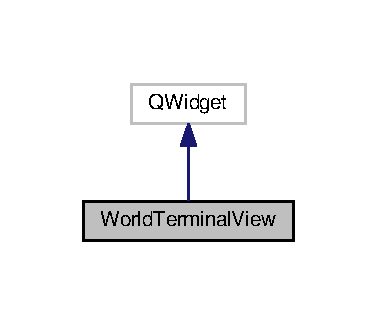
\includegraphics[width=181pt]{d8/da5/classWorldTerminalView__inherit__graph}
\end{center}
\end{figure}


Collaboration diagram for World\+Terminal\+View\+:\nopagebreak
\begin{figure}[H]
\begin{center}
\leavevmode
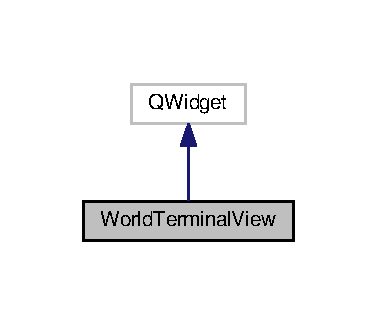
\includegraphics[width=181pt]{df/d82/classWorldTerminalView__coll__graph}
\end{center}
\end{figure}
\subsection*{Public Slots}
\begin{DoxyCompactItemize}
\item 
void \hyperlink{classWorldTerminalView_abca57ada64d0d466fad4e48b26283ee7}{on\+Return\+Pressed} ()\hypertarget{classWorldTerminalView_abca57ada64d0d466fad4e48b26283ee7}{}\label{classWorldTerminalView_abca57ada64d0d466fad4e48b26283ee7}

\begin{DoxyCompactList}\small\item\em Read and execute the typed command. \end{DoxyCompactList}\item 
void \hyperlink{classWorldTerminalView_a39a7a5c66e6184474cf5e43182cca8df}{on\+Enemy\+Defeated} (int x, int y)
\begin{DoxyCompactList}\small\item\em Print info on enemy defeated signal. \end{DoxyCompactList}\item 
void \hyperlink{classWorldTerminalView_ab6ebb9b798c452dbb7bc6859e6c0082c}{on\+Area\+Posioned} (int value, Q\+Rect rect)
\begin{DoxyCompactList}\small\item\em Print info on area\+Poisoned signal. \end{DoxyCompactList}\item 
void \hyperlink{classWorldTerminalView_a9d400f81edbf0b5f6f2779a71311dadf}{on\+Healthpack\+Used} (int x, int y)
\begin{DoxyCompactList}\small\item\em Print info on health\+Pack\+Used signal. \end{DoxyCompactList}\item 
void \hyperlink{classWorldTerminalView_a754cab62b8dbff71fce179c1307fefde}{on\+Health\+Level\+Changed} (int value)
\begin{DoxyCompactList}\small\item\em Print info on health\+Level\+Changed signal. \end{DoxyCompactList}\item 
void \hyperlink{classWorldTerminalView_acce60911ae9ec49a2d25c9df3d0a4aa7}{on\+Position\+Changed} (int x, int y)
\begin{DoxyCompactList}\small\item\em Print info on protagonist position changed. \end{DoxyCompactList}\item 
void \hyperlink{classWorldTerminalView_ac2a90b7f75ef680dfc3acb5ee56e022a}{reload\+View} ()\hypertarget{classWorldTerminalView_ac2a90b7f75ef680dfc3acb5ee56e022a}{}\label{classWorldTerminalView_ac2a90b7f75ef680dfc3acb5ee56e022a}

\begin{DoxyCompactList}\small\item\em Reload the view slot Reloads the view every time the model is reloaded. \end{DoxyCompactList}\end{DoxyCompactItemize}
\subsection*{Public Member Functions}
\begin{DoxyCompactItemize}
\item 
\hyperlink{classWorldTerminalView_a5cf7926b3cf66af1f036f976315fab99}{World\+Terminal\+View} (Q\+Widget $\ast$parent=0)
\begin{DoxyCompactList}\small\item\em Class constructor. \end{DoxyCompactList}\item 
void \hyperlink{classWorldTerminalView_ab9a76421814621d776d641e36946f0e4}{set\+Model} (\hyperlink{classWorldModel}{World\+Model} $\ast$m)
\begin{DoxyCompactList}\small\item\em Set model for the view. \end{DoxyCompactList}\item 
void \hyperlink{classWorldTerminalView_a8a52d3ddd8cef89f14123eb7c8fdaa41}{execute\+Cmd} (Q\+String \&cmd, Q\+String\+List args)
\begin{DoxyCompactList}\small\item\em Execute a command. \end{DoxyCompactList}\item 
void \hyperlink{classWorldTerminalView_a66913418f7408cb2d9abf989b1679163}{help} (Q\+String command=\char`\"{}\char`\"{})
\begin{DoxyCompactList}\small\item\em Print help on a command. \end{DoxyCompactList}\item 
void \hyperlink{classWorldTerminalView_a3b716b8dc01872822824e41115153742}{find} (Q\+String object, float value)
\begin{DoxyCompactList}\small\item\em Print information about a closest object. \end{DoxyCompactList}\item 
void \hyperlink{classWorldTerminalView_a549769ec34738ea2f4d39faddabeb0b3}{print\+Info} (Q\+String object)
\begin{DoxyCompactList}\small\item\em Print info about all objects of a given type. \end{DoxyCompactList}\end{DoxyCompactItemize}


\subsection{Detailed Description}
The \hyperlink{classWorldTerminalView}{World\+Terminal\+View} class. 

\subsection{Constructor \& Destructor Documentation}
\index{World\+Terminal\+View@{World\+Terminal\+View}!World\+Terminal\+View@{World\+Terminal\+View}}
\index{World\+Terminal\+View@{World\+Terminal\+View}!World\+Terminal\+View@{World\+Terminal\+View}}
\subsubsection[{\texorpdfstring{World\+Terminal\+View(\+Q\+Widget $\ast$parent=0)}{WorldTerminalView(QWidget *parent=0)}}]{\setlength{\rightskip}{0pt plus 5cm}World\+Terminal\+View\+::\+World\+Terminal\+View (
\begin{DoxyParamCaption}
\item[{Q\+Widget $\ast$}]{parent = {\ttfamily 0}}
\end{DoxyParamCaption}
)}\hypertarget{classWorldTerminalView_a5cf7926b3cf66af1f036f976315fab99}{}\label{classWorldTerminalView_a5cf7926b3cf66af1f036f976315fab99}


Class constructor. 


\begin{DoxyParams}{Parameters}
{\em parent} & parent object \\
\hline
\end{DoxyParams}


\subsection{Member Function Documentation}
\index{World\+Terminal\+View@{World\+Terminal\+View}!execute\+Cmd@{execute\+Cmd}}
\index{execute\+Cmd@{execute\+Cmd}!World\+Terminal\+View@{World\+Terminal\+View}}
\subsubsection[{\texorpdfstring{execute\+Cmd(\+Q\+String \&cmd, Q\+String\+List args)}{executeCmd(QString &cmd, QStringList args)}}]{\setlength{\rightskip}{0pt plus 5cm}void World\+Terminal\+View\+::execute\+Cmd (
\begin{DoxyParamCaption}
\item[{Q\+String \&}]{cmd, }
\item[{Q\+String\+List}]{args}
\end{DoxyParamCaption}
)}\hypertarget{classWorldTerminalView_a8a52d3ddd8cef89f14123eb7c8fdaa41}{}\label{classWorldTerminalView_a8a52d3ddd8cef89f14123eb7c8fdaa41}


Execute a command. 


\begin{DoxyParams}{Parameters}
{\em cmd} & Command string \\
\hline
{\em args} & Arguments \\
\hline
\end{DoxyParams}
\index{World\+Terminal\+View@{World\+Terminal\+View}!find@{find}}
\index{find@{find}!World\+Terminal\+View@{World\+Terminal\+View}}
\subsubsection[{\texorpdfstring{find(\+Q\+String object, float value)}{find(QString object, float value)}}]{\setlength{\rightskip}{0pt plus 5cm}void World\+Terminal\+View\+::find (
\begin{DoxyParamCaption}
\item[{Q\+String}]{object, }
\item[{float}]{value}
\end{DoxyParamCaption}
)}\hypertarget{classWorldTerminalView_a3b716b8dc01872822824e41115153742}{}\label{classWorldTerminalView_a3b716b8dc01872822824e41115153742}


Print information about a closest object. 

Print information about the closest object of a given type (e = any enemy, pe = poisoned enemy, re = regular enemy, h = health pack). 
\begin{DoxyParams}{Parameters}
{\em object} & type of object \\
\hline
{\em value} & threshold value of the object(minimal for health pack, maximal for enemy) \\
\hline
\end{DoxyParams}
\index{World\+Terminal\+View@{World\+Terminal\+View}!help@{help}}
\index{help@{help}!World\+Terminal\+View@{World\+Terminal\+View}}
\subsubsection[{\texorpdfstring{help(\+Q\+String command="""")}{help(QString command="")}}]{\setlength{\rightskip}{0pt plus 5cm}void World\+Terminal\+View\+::help (
\begin{DoxyParamCaption}
\item[{Q\+String}]{command = {\ttfamily \char`\"{}\char`\"{}}}
\end{DoxyParamCaption}
)}\hypertarget{classWorldTerminalView_a66913418f7408cb2d9abf989b1679163}{}\label{classWorldTerminalView_a66913418f7408cb2d9abf989b1679163}


Print help on a command. 


\begin{DoxyParams}{Parameters}
{\em command} & command name(print overall help if no command is sepcified) \\
\hline
\end{DoxyParams}
\index{World\+Terminal\+View@{World\+Terminal\+View}!on\+Area\+Posioned@{on\+Area\+Posioned}}
\index{on\+Area\+Posioned@{on\+Area\+Posioned}!World\+Terminal\+View@{World\+Terminal\+View}}
\subsubsection[{\texorpdfstring{on\+Area\+Posioned}{onAreaPosioned}}]{\setlength{\rightskip}{0pt plus 5cm}void World\+Terminal\+View\+::on\+Area\+Posioned (
\begin{DoxyParamCaption}
\item[{int}]{value, }
\item[{Q\+Rect}]{rect}
\end{DoxyParamCaption}
)\hspace{0.3cm}{\ttfamily [slot]}}\hypertarget{classWorldTerminalView_ab6ebb9b798c452dbb7bc6859e6c0082c}{}\label{classWorldTerminalView_ab6ebb9b798c452dbb7bc6859e6c0082c}


Print info on area\+Poisoned signal. 


\begin{DoxyParams}{Parameters}
{\em value} & poison level \\
\hline
{\em rect} & poisoned area \\
\hline
\end{DoxyParams}
\index{World\+Terminal\+View@{World\+Terminal\+View}!on\+Enemy\+Defeated@{on\+Enemy\+Defeated}}
\index{on\+Enemy\+Defeated@{on\+Enemy\+Defeated}!World\+Terminal\+View@{World\+Terminal\+View}}
\subsubsection[{\texorpdfstring{on\+Enemy\+Defeated}{onEnemyDefeated}}]{\setlength{\rightskip}{0pt plus 5cm}void World\+Terminal\+View\+::on\+Enemy\+Defeated (
\begin{DoxyParamCaption}
\item[{int}]{x, }
\item[{int}]{y}
\end{DoxyParamCaption}
)\hspace{0.3cm}{\ttfamily [slot]}}\hypertarget{classWorldTerminalView_a39a7a5c66e6184474cf5e43182cca8df}{}\label{classWorldTerminalView_a39a7a5c66e6184474cf5e43182cca8df}


Print info on enemy defeated signal. 


\begin{DoxyParams}{Parameters}
{\em x} & horizontal position of the enemy \\
\hline
{\em y} & vertical position of the enemy \\
\hline
\end{DoxyParams}
\index{World\+Terminal\+View@{World\+Terminal\+View}!on\+Health\+Level\+Changed@{on\+Health\+Level\+Changed}}
\index{on\+Health\+Level\+Changed@{on\+Health\+Level\+Changed}!World\+Terminal\+View@{World\+Terminal\+View}}
\subsubsection[{\texorpdfstring{on\+Health\+Level\+Changed}{onHealthLevelChanged}}]{\setlength{\rightskip}{0pt plus 5cm}void World\+Terminal\+View\+::on\+Health\+Level\+Changed (
\begin{DoxyParamCaption}
\item[{int}]{value}
\end{DoxyParamCaption}
)\hspace{0.3cm}{\ttfamily [slot]}}\hypertarget{classWorldTerminalView_a754cab62b8dbff71fce179c1307fefde}{}\label{classWorldTerminalView_a754cab62b8dbff71fce179c1307fefde}


Print info on health\+Level\+Changed signal. 


\begin{DoxyParams}{Parameters}
{\em value} & health level \\
\hline
\end{DoxyParams}
\index{World\+Terminal\+View@{World\+Terminal\+View}!on\+Healthpack\+Used@{on\+Healthpack\+Used}}
\index{on\+Healthpack\+Used@{on\+Healthpack\+Used}!World\+Terminal\+View@{World\+Terminal\+View}}
\subsubsection[{\texorpdfstring{on\+Healthpack\+Used}{onHealthpackUsed}}]{\setlength{\rightskip}{0pt plus 5cm}void World\+Terminal\+View\+::on\+Healthpack\+Used (
\begin{DoxyParamCaption}
\item[{int}]{x, }
\item[{int}]{y}
\end{DoxyParamCaption}
)\hspace{0.3cm}{\ttfamily [slot]}}\hypertarget{classWorldTerminalView_a9d400f81edbf0b5f6f2779a71311dadf}{}\label{classWorldTerminalView_a9d400f81edbf0b5f6f2779a71311dadf}


Print info on health\+Pack\+Used signal. 


\begin{DoxyParams}{Parameters}
{\em x} & horizontal position of the health pack \\
\hline
{\em y} & vertical position of the health pack \\
\hline
\end{DoxyParams}
\index{World\+Terminal\+View@{World\+Terminal\+View}!on\+Position\+Changed@{on\+Position\+Changed}}
\index{on\+Position\+Changed@{on\+Position\+Changed}!World\+Terminal\+View@{World\+Terminal\+View}}
\subsubsection[{\texorpdfstring{on\+Position\+Changed}{onPositionChanged}}]{\setlength{\rightskip}{0pt plus 5cm}void World\+Terminal\+View\+::on\+Position\+Changed (
\begin{DoxyParamCaption}
\item[{int}]{x, }
\item[{int}]{y}
\end{DoxyParamCaption}
)\hspace{0.3cm}{\ttfamily [slot]}}\hypertarget{classWorldTerminalView_acce60911ae9ec49a2d25c9df3d0a4aa7}{}\label{classWorldTerminalView_acce60911ae9ec49a2d25c9df3d0a4aa7}


Print info on protagonist position changed. 


\begin{DoxyParams}{Parameters}
{\em x} & horizontal position of the protagonist \\
\hline
{\em y} & vertical position of the protagonist \\
\hline
\end{DoxyParams}
\index{World\+Terminal\+View@{World\+Terminal\+View}!print\+Info@{print\+Info}}
\index{print\+Info@{print\+Info}!World\+Terminal\+View@{World\+Terminal\+View}}
\subsubsection[{\texorpdfstring{print\+Info(\+Q\+String object)}{printInfo(QString object)}}]{\setlength{\rightskip}{0pt plus 5cm}void World\+Terminal\+View\+::print\+Info (
\begin{DoxyParamCaption}
\item[{Q\+String}]{object}
\end{DoxyParamCaption}
)}\hypertarget{classWorldTerminalView_a549769ec34738ea2f4d39faddabeb0b3}{}\label{classWorldTerminalView_a549769ec34738ea2f4d39faddabeb0b3}


Print info about all objects of a given type. 


\begin{DoxyItemize}
\item Print information about all objects of a given type (e = all enemies, pe = poisoned enemies, re = regular enemies, h = health packs). 
\begin{DoxyParams}{Parameters}
{\em object} & type of object \\
\hline
\end{DoxyParams}

\end{DoxyItemize}\index{World\+Terminal\+View@{World\+Terminal\+View}!set\+Model@{set\+Model}}
\index{set\+Model@{set\+Model}!World\+Terminal\+View@{World\+Terminal\+View}}
\subsubsection[{\texorpdfstring{set\+Model(\+World\+Model $\ast$m)}{setModel(WorldModel *m)}}]{\setlength{\rightskip}{0pt plus 5cm}void World\+Terminal\+View\+::set\+Model (
\begin{DoxyParamCaption}
\item[{{\bf World\+Model} $\ast$}]{m}
\end{DoxyParamCaption}
)}\hypertarget{classWorldTerminalView_ab9a76421814621d776d641e36946f0e4}{}\label{classWorldTerminalView_ab9a76421814621d776d641e36946f0e4}


Set model for the view. 


\begin{DoxyParams}{Parameters}
{\em m} & model \\
\hline
\end{DoxyParams}


The documentation for this class was generated from the following files\+:\begin{DoxyCompactItemize}
\item 
/home/bobiko/ku-\/leuven/media-\/processing/labs/finaltask/finaltask/src/terminalview/\hyperlink{worldterminalview_8h}{worldterminalview.\+h}\item 
/home/bobiko/ku-\/leuven/media-\/processing/labs/finaltask/finaltask/src/terminalview/\hyperlink{worldterminalview_8cpp}{worldterminalview.\+cpp}\end{DoxyCompactItemize}

\chapter{File Documentation}
\hypertarget{astarcontroller_8cpp}{}\section{/home/bobiko/ku-\/leuven/media-\/processing/labs/finaltask/finaltask/src/controller/astarcontroller.cpp File Reference}
\label{astarcontroller_8cpp}\index{/home/bobiko/ku-\/leuven/media-\/processing/labs/finaltask/finaltask/src/controller/astarcontroller.\+cpp@{/home/bobiko/ku-\/leuven/media-\/processing/labs/finaltask/finaltask/src/controller/astarcontroller.\+cpp}}
{\ttfamily \#include \char`\"{}astarcontroller.\+h\char`\"{}}\\*
{\ttfamily \#include \char`\"{}model/worldmodel.\+h\char`\"{}}\\*
Include dependency graph for astarcontroller.\+cpp\+:\nopagebreak
\begin{figure}[H]
\begin{center}
\leavevmode
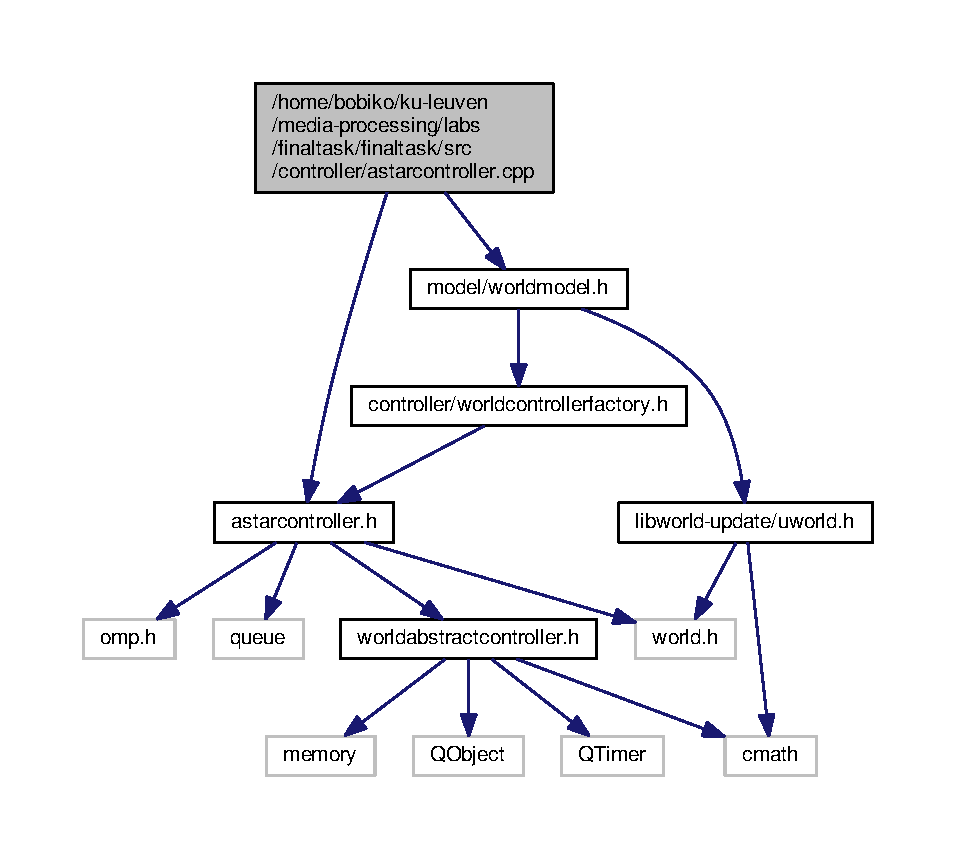
\includegraphics[width=350pt]{dd/d3a/astarcontroller_8cpp__incl}
\end{center}
\end{figure}


\subsection{Detailed Description}
\hyperlink{classWorldControllerFactory}{World\+Controller\+Factory} class definition

\begin{DoxyVersion}{Version}
1.\+0
\end{DoxyVersion}
\begin{DoxyAuthor}{Author}
Vladimir Poliakov 

Brian Segers 

Kasper De Volder 
\end{DoxyAuthor}

\hypertarget{astarcontroller_8h}{}\section{/home/bobiko/ku-\/leuven/media-\/processing/labs/finaltask/finaltask/src/controller/astarcontroller.h File Reference}
\label{astarcontroller_8h}\index{/home/bobiko/ku-\/leuven/media-\/processing/labs/finaltask/finaltask/src/controller/astarcontroller.\+h@{/home/bobiko/ku-\/leuven/media-\/processing/labs/finaltask/finaltask/src/controller/astarcontroller.\+h}}
{\ttfamily \#include $<$omp.\+h$>$}\\*
{\ttfamily \#include $<$queue$>$}\\*
{\ttfamily \#include \char`\"{}worldabstractcontroller.\+h\char`\"{}}\\*
{\ttfamily \#include \char`\"{}world.\+h\char`\"{}}\\*
Include dependency graph for astarcontroller.\+h\+:\nopagebreak
\begin{figure}[H]
\begin{center}
\leavevmode
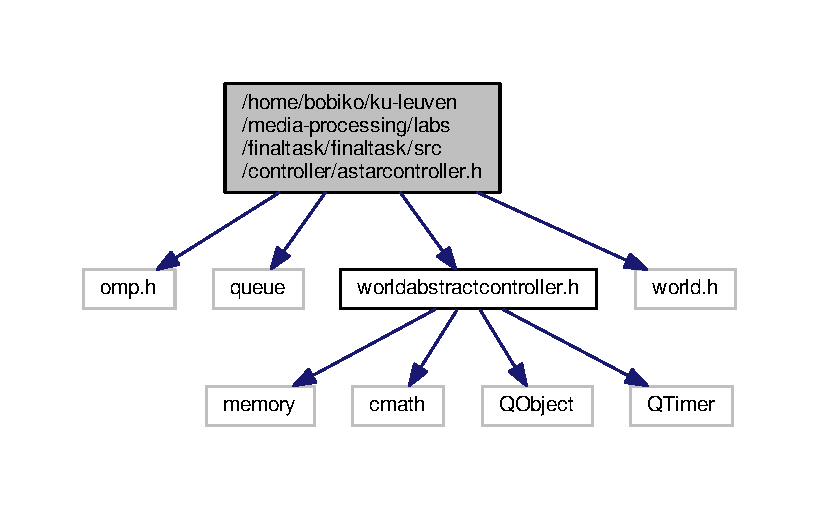
\includegraphics[width=350pt]{d5/dae/astarcontroller_8h__incl}
\end{center}
\end{figure}
This graph shows which files directly or indirectly include this file\+:\nopagebreak
\begin{figure}[H]
\begin{center}
\leavevmode
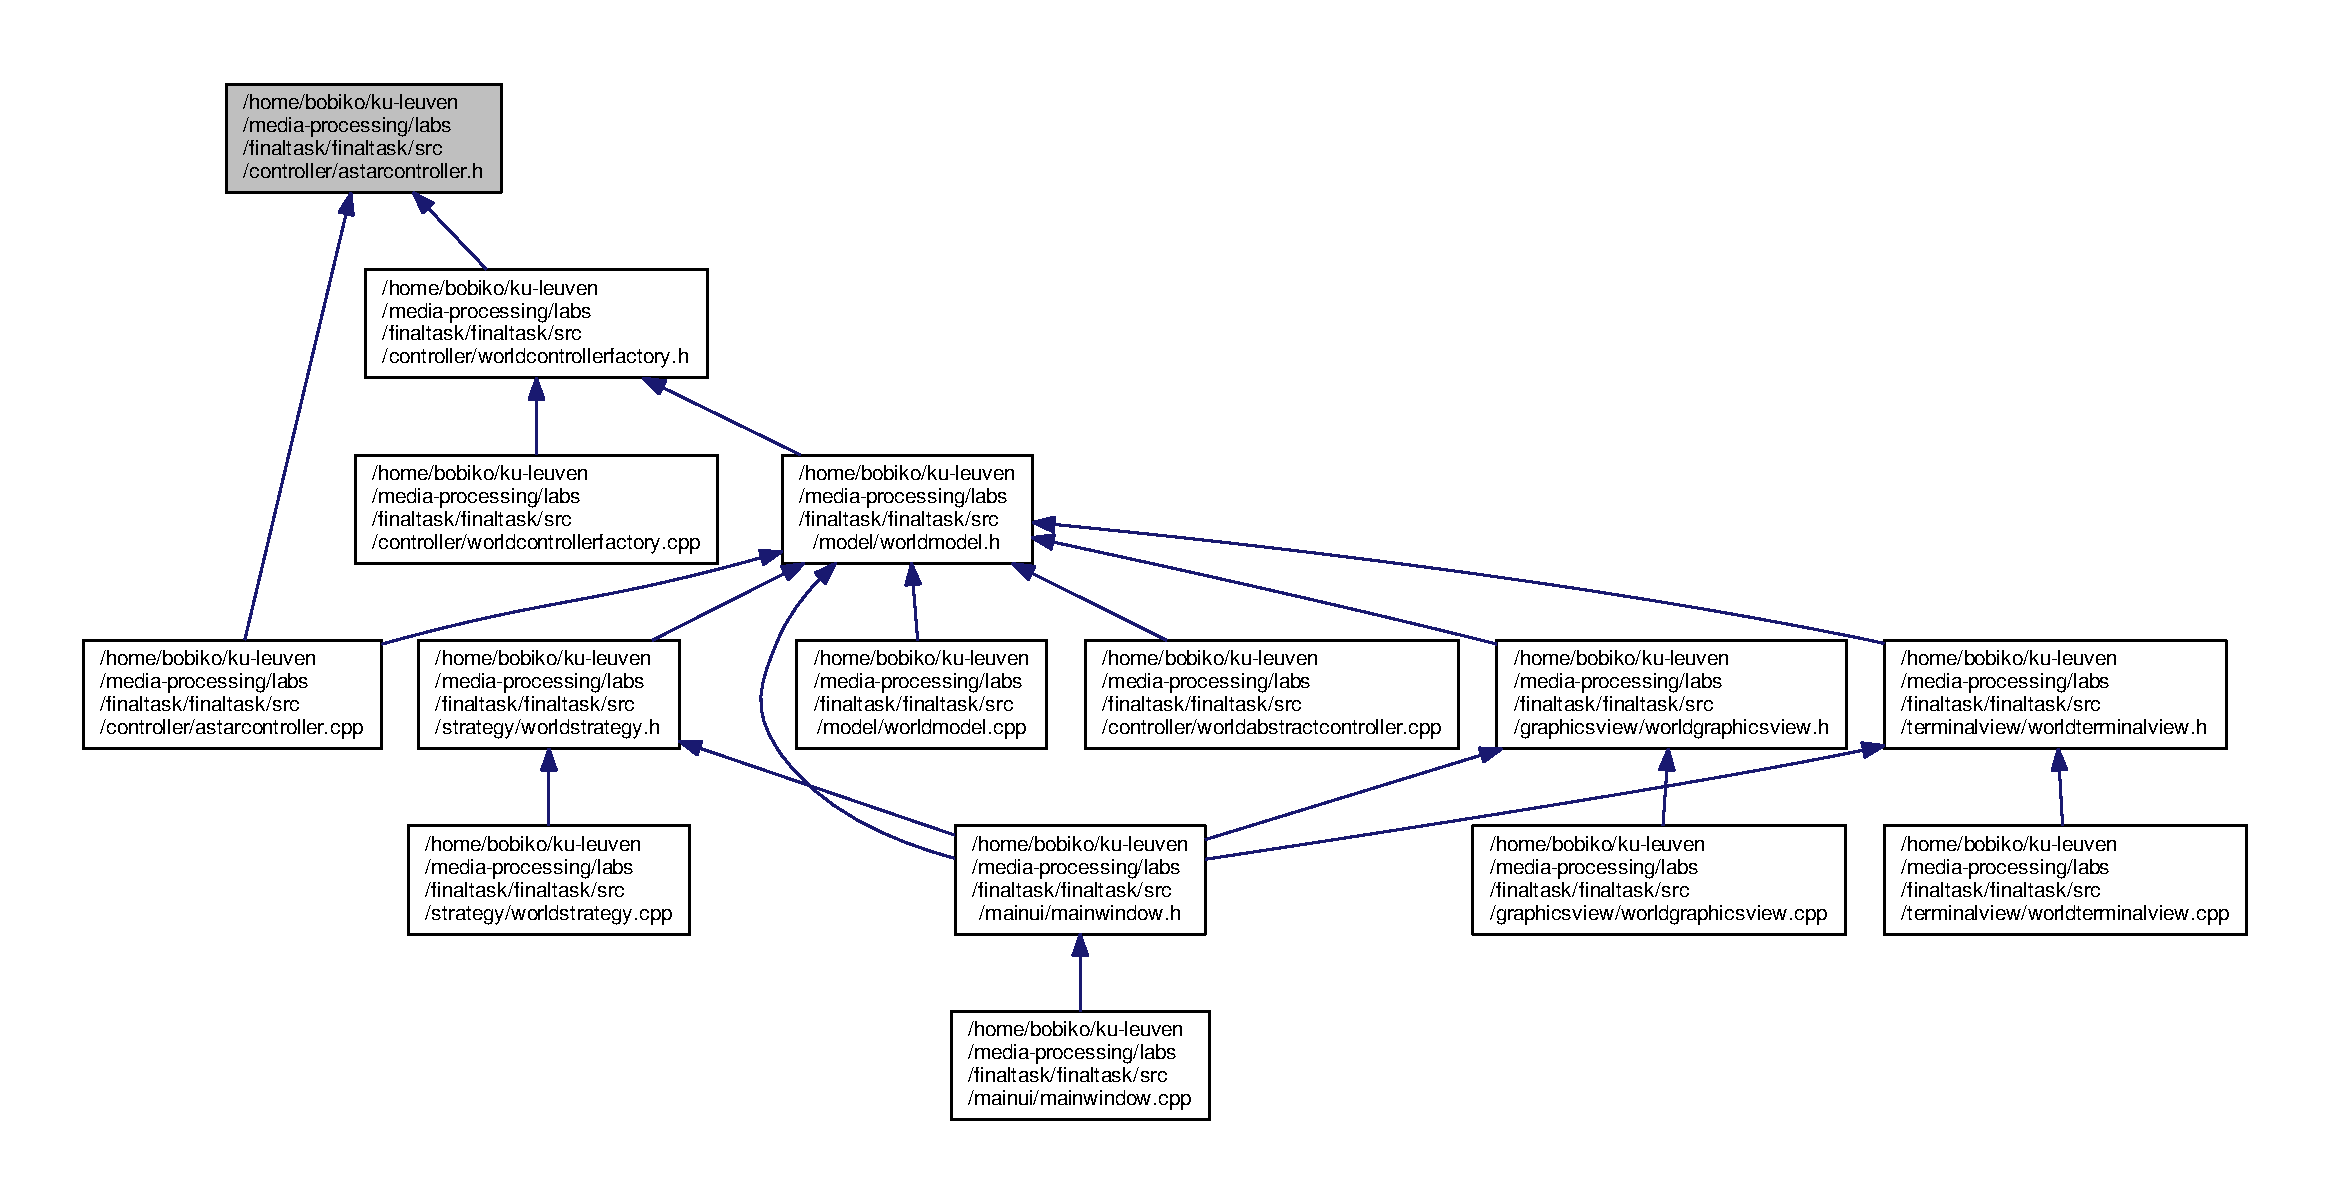
\includegraphics[width=350pt]{dc/d82/astarcontroller_8h__dep__incl}
\end{center}
\end{figure}
\subsection*{Classes}
\begin{DoxyCompactItemize}
\item 
struct \hyperlink{structNode}{Node}
\begin{DoxyCompactList}\small\item\em The \hyperlink{structNode}{Node} struct. \end{DoxyCompactList}\item 
class \hyperlink{classCompareCost}{Compare\+Cost}
\begin{DoxyCompactList}\small\item\em \hyperlink{structNode}{Node} comparison functor. \end{DoxyCompactList}\item 
class \hyperlink{classAStarController}{A\+Star\+Controller}
\begin{DoxyCompactList}\small\item\em A$\ast$ controller. \end{DoxyCompactList}\end{DoxyCompactItemize}


\subsection{Detailed Description}
\hyperlink{classAStarController}{A\+Star\+Controller} class declaration

\begin{DoxyVersion}{Version}
1.\+0
\end{DoxyVersion}
\begin{DoxyAuthor}{Author}
Vladimir Poliakov 

Brian Segers 

Kasper De Volder 
\end{DoxyAuthor}

\hypertarget{worldabstractcontroller_8cpp}{}\section{/home/bobiko/ku-\/leuven/media-\/processing/labs/finaltask/finaltask/src/controller/worldabstractcontroller.cpp File Reference}
\label{worldabstractcontroller_8cpp}\index{/home/bobiko/ku-\/leuven/media-\/processing/labs/finaltask/finaltask/src/controller/worldabstractcontroller.\+cpp@{/home/bobiko/ku-\/leuven/media-\/processing/labs/finaltask/finaltask/src/controller/worldabstractcontroller.\+cpp}}
{\ttfamily \#include \char`\"{}worldabstractcontroller.\+h\char`\"{}}\\*
{\ttfamily \#include \char`\"{}model/worldmodel.\+h\char`\"{}}\\*
Include dependency graph for worldabstractcontroller.\+cpp\+:
\nopagebreak
\begin{figure}[H]
\begin{center}
\leavevmode
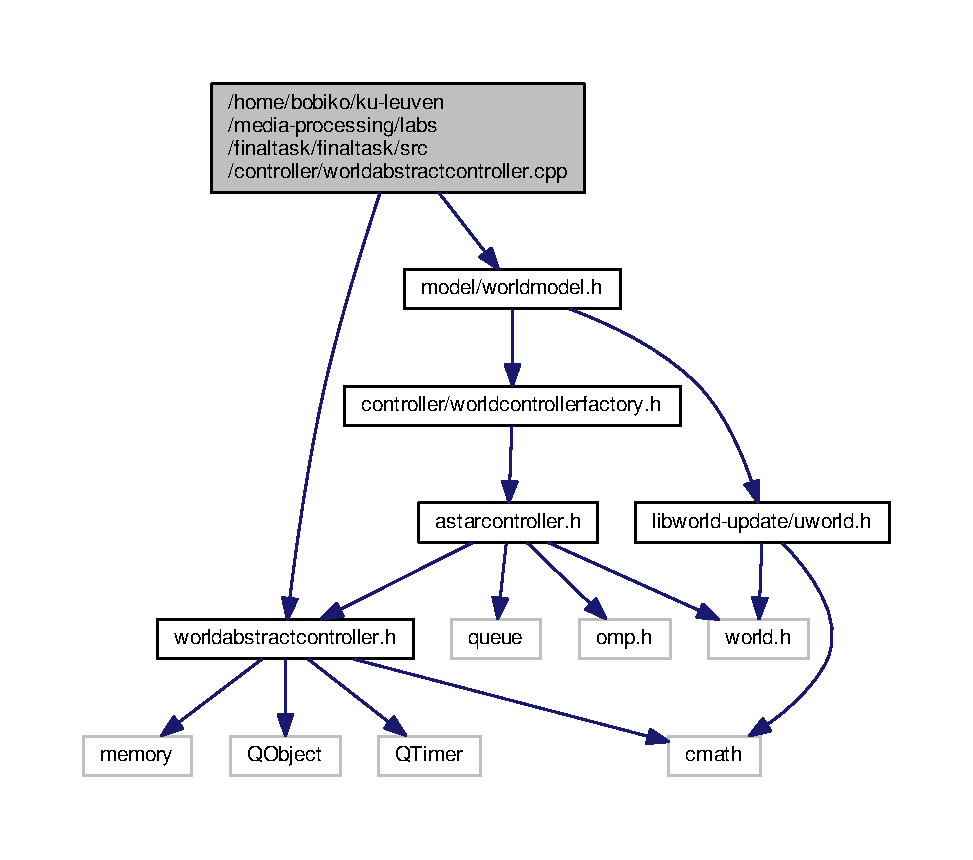
\includegraphics[width=350pt]{d0/d44/worldabstractcontroller_8cpp__incl}
\end{center}
\end{figure}


\subsection{Detailed Description}
\hyperlink{classWorldAbstractController}{World\+Abstract\+Controller} class definition

\begin{DoxyVersion}{Version}
1.\+0
\end{DoxyVersion}
\begin{DoxyAuthor}{Author}
Vladimir Poliakov 

Brian Segers 

Kasper De Volder 
\end{DoxyAuthor}

\hypertarget{worldabstractcontroller_8h}{}\section{/home/bobiko/ku-\/leuven/media-\/processing/labs/finaltask/finaltask/src/controller/worldabstractcontroller.h File Reference}
\label{worldabstractcontroller_8h}\index{/home/bobiko/ku-\/leuven/media-\/processing/labs/finaltask/finaltask/src/controller/worldabstractcontroller.\+h@{/home/bobiko/ku-\/leuven/media-\/processing/labs/finaltask/finaltask/src/controller/worldabstractcontroller.\+h}}
{\ttfamily \#include $<$memory$>$}\\*
{\ttfamily \#include $<$Q\+Object$>$}\\*
{\ttfamily \#include $<$Q\+Vector$>$}\\*
{\ttfamily \#include $<$Q\+Timer$>$}\\*
Include dependency graph for worldabstractcontroller.\+h\+:
\nopagebreak
\begin{figure}[H]
\begin{center}
\leavevmode
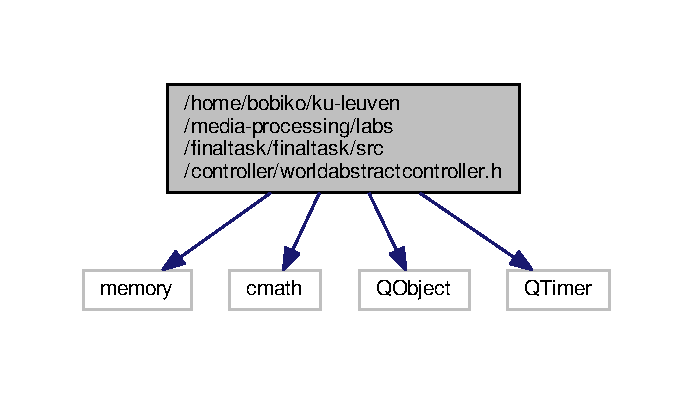
\includegraphics[width=342pt]{d9/d56/worldabstractcontroller_8h__incl}
\end{center}
\end{figure}
This graph shows which files directly or indirectly include this file\+:
\nopagebreak
\begin{figure}[H]
\begin{center}
\leavevmode
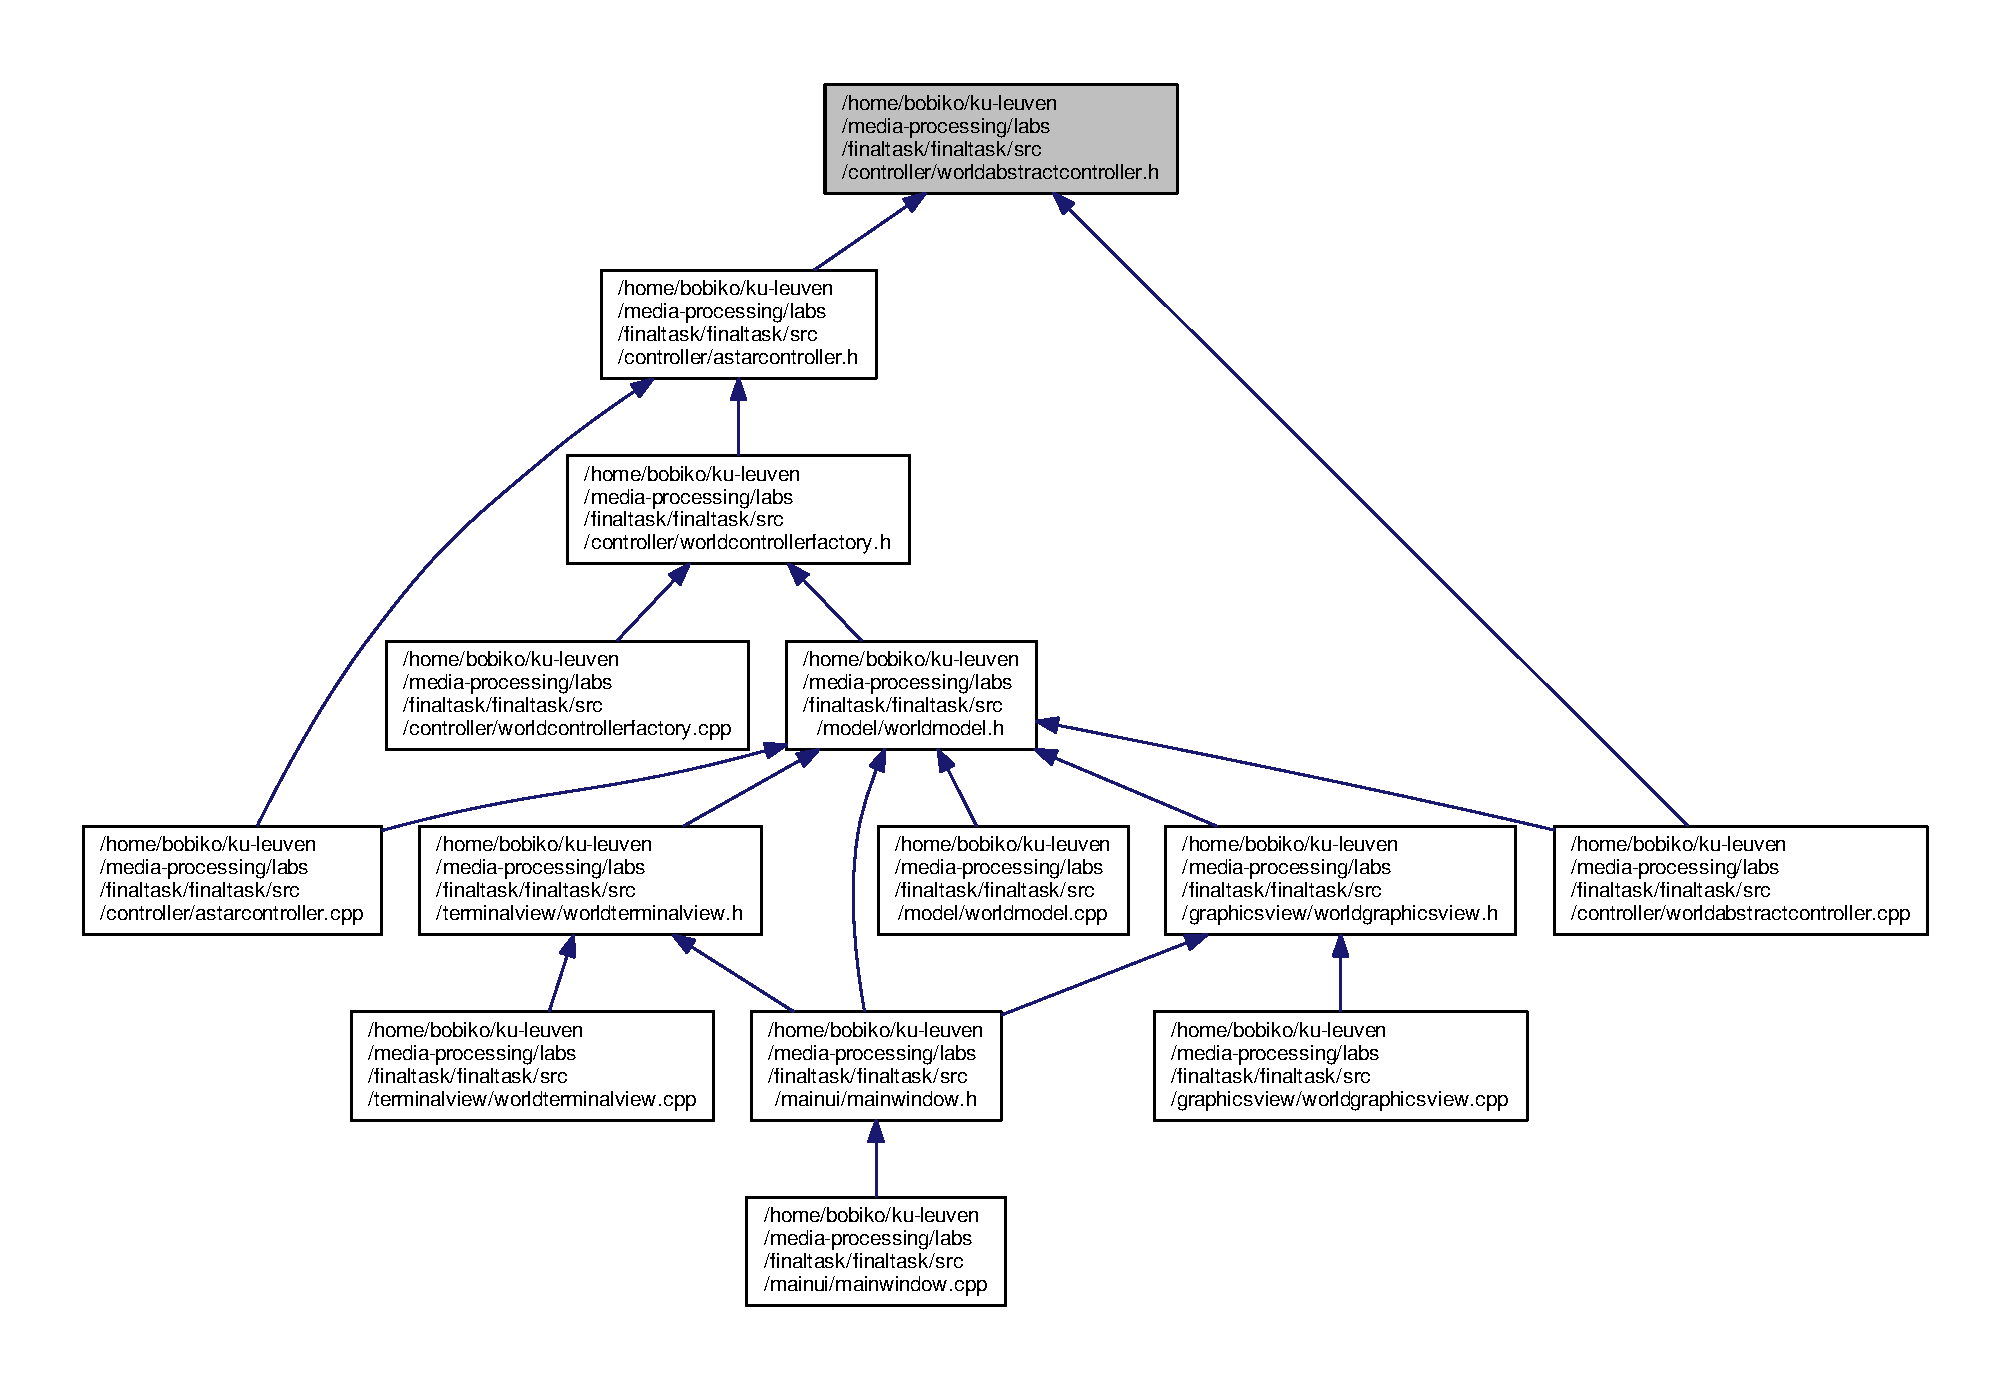
\includegraphics[width=350pt]{d7/d32/worldabstractcontroller_8h__dep__incl}
\end{center}
\end{figure}
\subsection*{Classes}
\begin{DoxyCompactItemize}
\item 
struct \hyperlink{structPath}{Path}
\begin{DoxyCompactList}\small\item\em The \hyperlink{structPath}{Path} struct. \end{DoxyCompactList}\item 
class \hyperlink{classWorldAbstractController}{World\+Abstract\+Controller}
\begin{DoxyCompactList}\small\item\em Abstract controller class. \end{DoxyCompactList}\end{DoxyCompactItemize}
\subsection*{Enumerations}
\begin{DoxyCompactItemize}
\item 
enum \hyperlink{worldabstractcontroller_8h_a842c5e2e69277690b064bf363c017980}{Object\+Type} \{ {\bfseries Health\+Pack}, 
{\bfseries Regular\+Enemy}, 
{\bfseries Poisoned\+Enemy}, 
{\bfseries Any\+Enemy}
 \}\begin{DoxyCompactList}\small\item\em Object type enumeration. \end{DoxyCompactList}
\end{DoxyCompactItemize}


\subsection{Detailed Description}
\hyperlink{classWorldAbstractController}{World\+Abstract\+Controller} class declaration

\begin{DoxyVersion}{Version}
1.\+0
\end{DoxyVersion}
\begin{DoxyAuthor}{Author}
Vladimir Poliakov 

Brian Segers 

Kasper De Volder 
\end{DoxyAuthor}


\subsection{Enumeration Type Documentation}
\index{worldabstractcontroller.\+h@{worldabstractcontroller.\+h}!Object\+Type@{Object\+Type}}
\index{Object\+Type@{Object\+Type}!worldabstractcontroller.\+h@{worldabstractcontroller.\+h}}
\subsubsection[{\texorpdfstring{Object\+Type}{ObjectType}}]{\setlength{\rightskip}{0pt plus 5cm}enum {\bf Object\+Type}}\hypertarget{worldabstractcontroller_8h_a842c5e2e69277690b064bf363c017980}{}\label{worldabstractcontroller_8h_a842c5e2e69277690b064bf363c017980}


Object type enumeration. 

Defines the type of object to search for

\begin{DoxySeeAlso}{See also}
find\+Closest 
\end{DoxySeeAlso}

\hypertarget{worldcontrollerfactory_8cpp}{}\section{/home/bobiko/ku-\/leuven/media-\/processing/labs/finaltask/finaltask/src/controller/worldcontrollerfactory.cpp File Reference}
\label{worldcontrollerfactory_8cpp}\index{/home/bobiko/ku-\/leuven/media-\/processing/labs/finaltask/finaltask/src/controller/worldcontrollerfactory.\+cpp@{/home/bobiko/ku-\/leuven/media-\/processing/labs/finaltask/finaltask/src/controller/worldcontrollerfactory.\+cpp}}
{\ttfamily \#include \char`\"{}worldcontrollerfactory.\+h\char`\"{}}\\*
Include dependency graph for worldcontrollerfactory.\+cpp\+:
\nopagebreak
\begin{figure}[H]
\begin{center}
\leavevmode
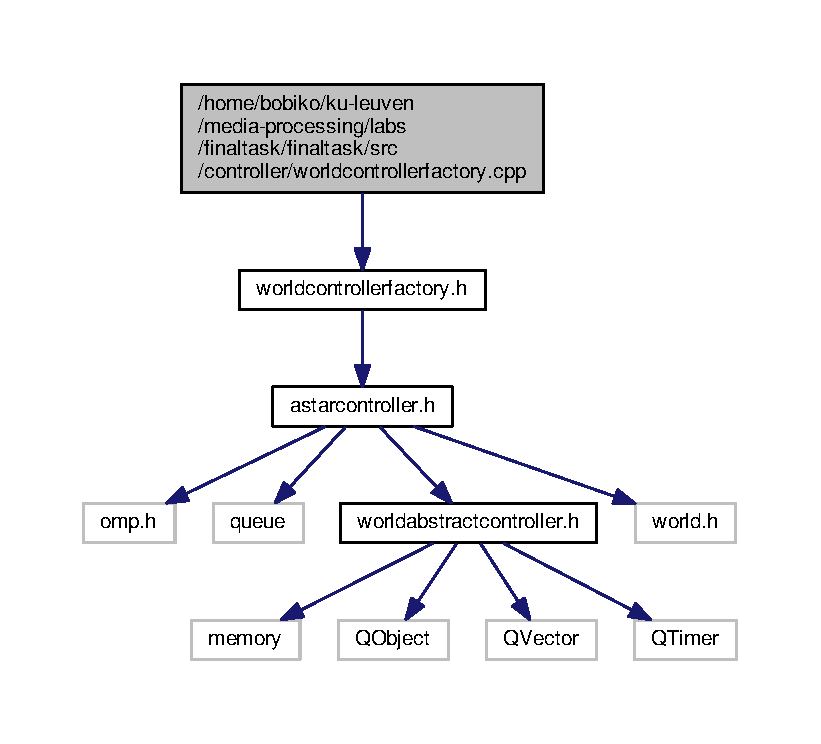
\includegraphics[width=350pt]{d5/ddc/worldcontrollerfactory_8cpp__incl}
\end{center}
\end{figure}


\subsection{Detailed Description}
\hyperlink{classWorldControllerFactory}{World\+Controller\+Factory} class definition

\begin{DoxyVersion}{Version}
1.\+0
\end{DoxyVersion}
\begin{DoxyAuthor}{Author}
Vladimir Poliakov 

Brian Segers 

Kasper De Volder 
\end{DoxyAuthor}

\hypertarget{worldcontrollerfactory_8h}{}\section{/home/bobiko/ku-\/leuven/media-\/processing/labs/finaltask/finaltask/src/controller/worldcontrollerfactory.h File Reference}
\label{worldcontrollerfactory_8h}\index{/home/bobiko/ku-\/leuven/media-\/processing/labs/finaltask/finaltask/src/controller/worldcontrollerfactory.\+h@{/home/bobiko/ku-\/leuven/media-\/processing/labs/finaltask/finaltask/src/controller/worldcontrollerfactory.\+h}}
{\ttfamily \#include \char`\"{}astarcontroller.\+h\char`\"{}}\\*
Include dependency graph for worldcontrollerfactory.\+h\+:
\nopagebreak
\begin{figure}[H]
\begin{center}
\leavevmode
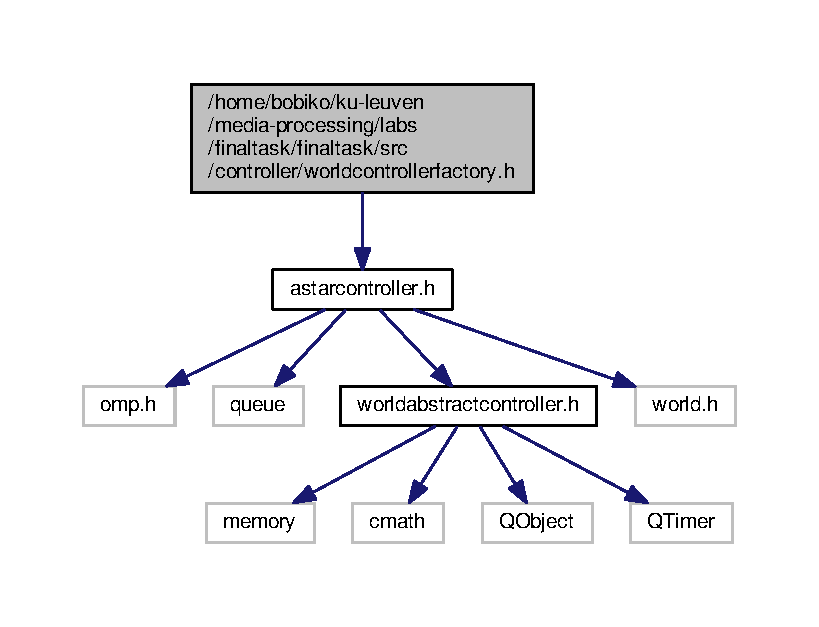
\includegraphics[width=350pt]{d8/deb/worldcontrollerfactory_8h__incl}
\end{center}
\end{figure}
This graph shows which files directly or indirectly include this file\+:
\nopagebreak
\begin{figure}[H]
\begin{center}
\leavevmode
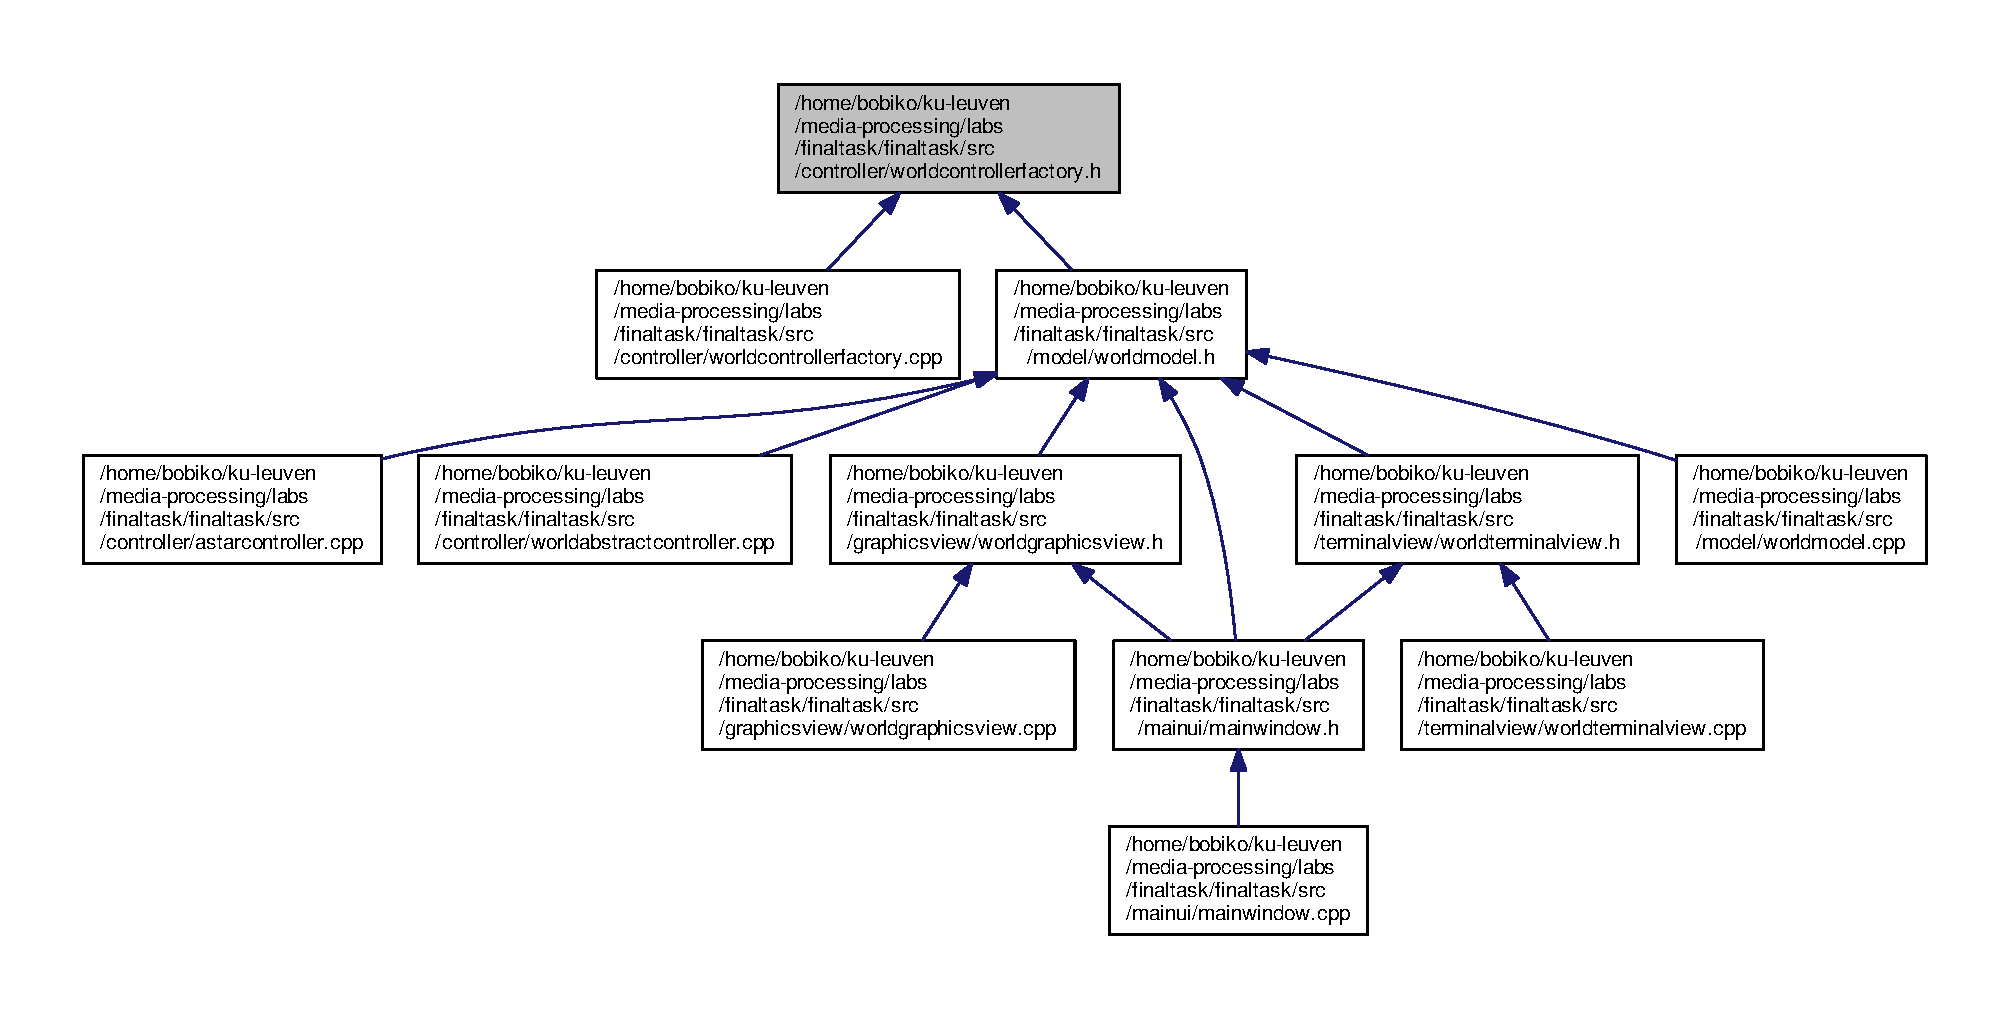
\includegraphics[width=350pt]{da/d6f/worldcontrollerfactory_8h__dep__incl}
\end{center}
\end{figure}
\subsection*{Classes}
\begin{DoxyCompactItemize}
\item 
class \hyperlink{classWorldControllerFactory}{World\+Controller\+Factory}
\begin{DoxyCompactList}\small\item\em Controller factory class. \end{DoxyCompactList}\end{DoxyCompactItemize}
\subsection*{Enumerations}
\begin{DoxyCompactItemize}
\item 
enum \hyperlink{group__controller_ga81059b4122c9dd4608d347eb117ae8c9}{Controller\+Type} \{ {\bfseries A\+Star}
 \}\begin{DoxyCompactList}\small\item\em The Controller\+Type enum. \end{DoxyCompactList}
\end{DoxyCompactItemize}


\subsection{Detailed Description}
\hyperlink{classWorldControllerFactory}{World\+Controller\+Factory} class declaration

\begin{DoxyVersion}{Version}
1.\+0
\end{DoxyVersion}
\begin{DoxyAuthor}{Author}
Vladimir Poliakov 

Brian Segers 

Kasper De Volder 
\end{DoxyAuthor}

\hypertarget{worldgraphicsview_8cpp}{}\section{/home/bobiko/ku-\/leuven/media-\/processing/labs/finaltask/finaltask/src/graphicsview/worldgraphicsview.cpp File Reference}
\label{worldgraphicsview_8cpp}\index{/home/bobiko/ku-\/leuven/media-\/processing/labs/finaltask/finaltask/src/graphicsview/worldgraphicsview.\+cpp@{/home/bobiko/ku-\/leuven/media-\/processing/labs/finaltask/finaltask/src/graphicsview/worldgraphicsview.\+cpp}}
{\ttfamily \#include \char`\"{}worldgraphicsview.\+h\char`\"{}}\\*
Include dependency graph for worldgraphicsview.\+cpp\+:
\nopagebreak
\begin{figure}[H]
\begin{center}
\leavevmode
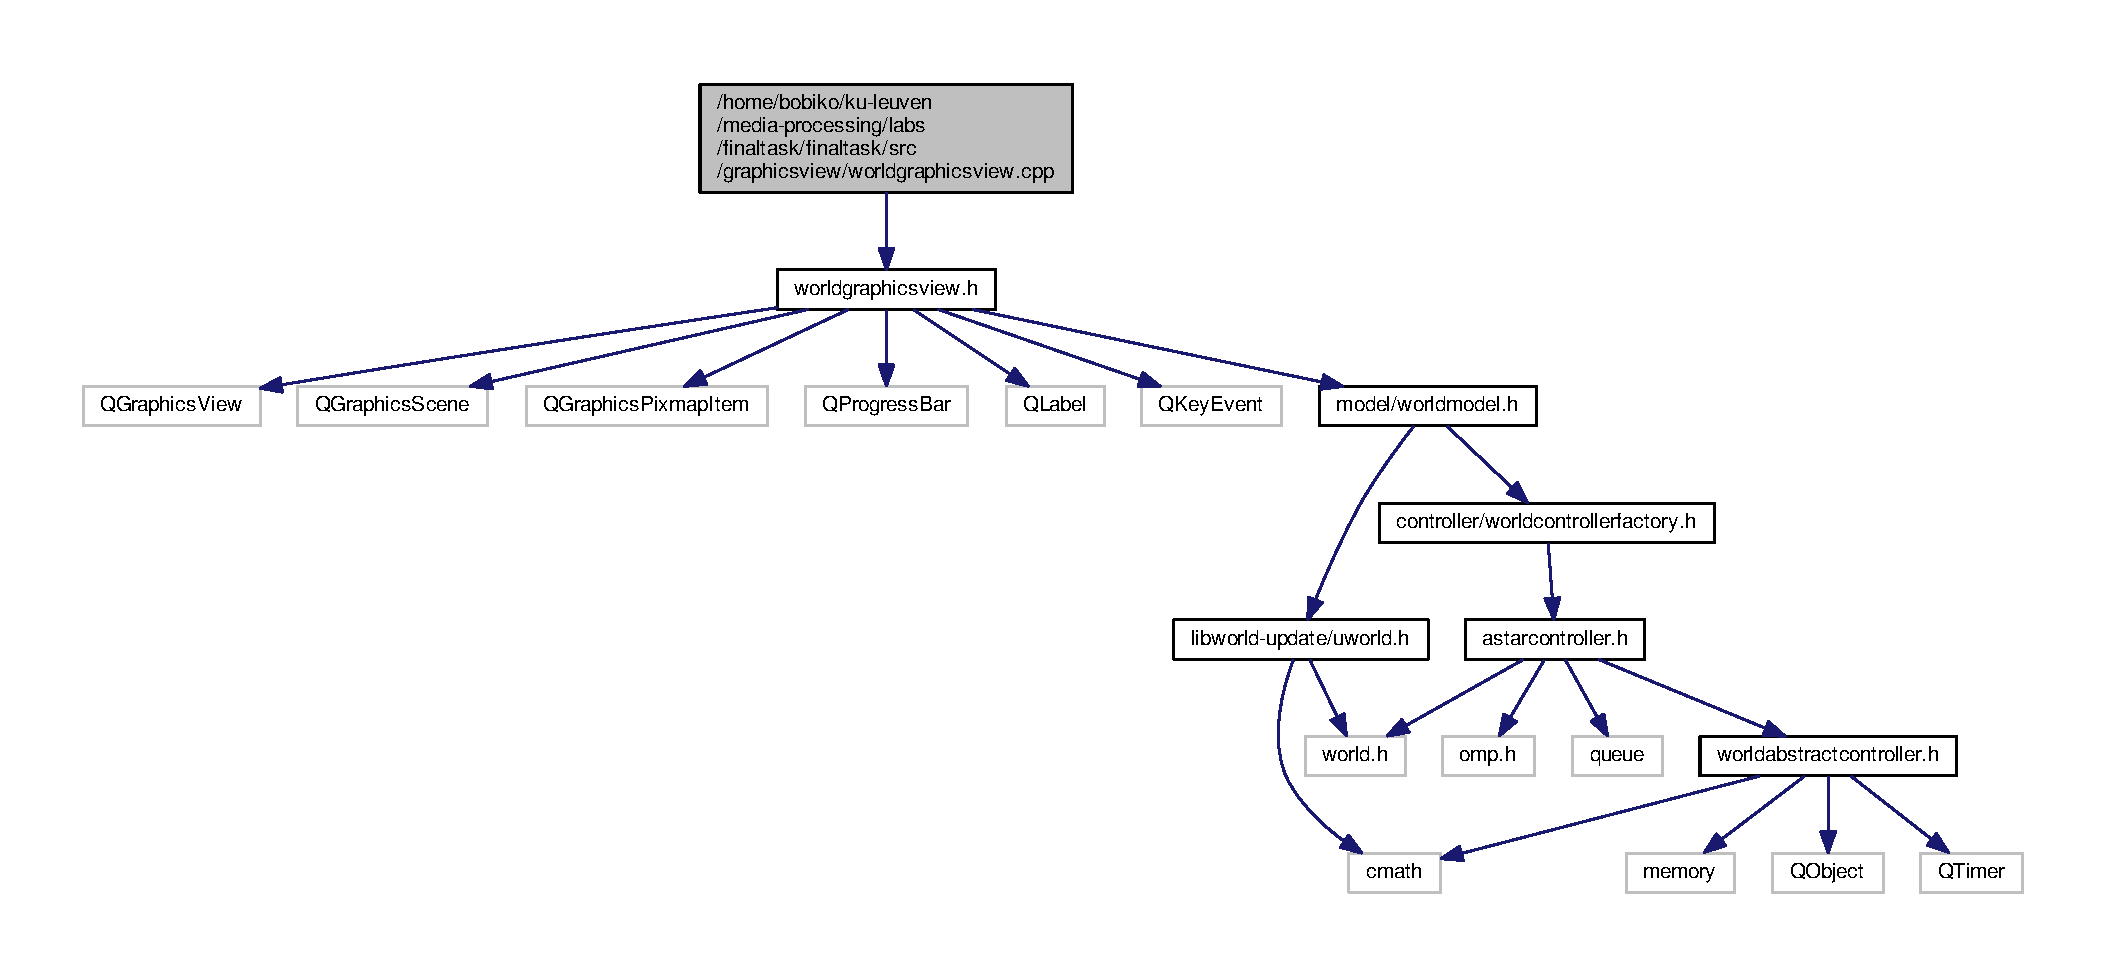
\includegraphics[width=350pt]{d1/de0/worldgraphicsview_8cpp__incl}
\end{center}
\end{figure}


\subsection{Detailed Description}
\hyperlink{classWorldGraphicsView}{World\+Graphics\+View} class definition

\begin{DoxyVersion}{Version}
1.\+0
\end{DoxyVersion}
\begin{DoxyAuthor}{Author}
Vladimir Poliakov 

Brian Segers 

Kasper De Volder 
\end{DoxyAuthor}

\hypertarget{worldgraphicsview_8h}{}\section{/home/bobiko/ku-\/leuven/media-\/processing/labs/finaltask/finaltask/src/graphicsview/worldgraphicsview.h File Reference}
\label{worldgraphicsview_8h}\index{/home/bobiko/ku-\/leuven/media-\/processing/labs/finaltask/finaltask/src/graphicsview/worldgraphicsview.\+h@{/home/bobiko/ku-\/leuven/media-\/processing/labs/finaltask/finaltask/src/graphicsview/worldgraphicsview.\+h}}
{\ttfamily \#include $<$Q\+Graphics\+View$>$}\\*
{\ttfamily \#include $<$Q\+Graphics\+Scene$>$}\\*
{\ttfamily \#include $<$Q\+Graphics\+Pixmap\+Item$>$}\\*
{\ttfamily \#include $<$Q\+Progress\+Bar$>$}\\*
{\ttfamily \#include $<$Q\+Label$>$}\\*
{\ttfamily \#include $<$Q\+Key\+Event$>$}\\*
{\ttfamily \#include \char`\"{}model/worldmodel.\+h\char`\"{}}\\*
Include dependency graph for worldgraphicsview.\+h\+:
\nopagebreak
\begin{figure}[H]
\begin{center}
\leavevmode
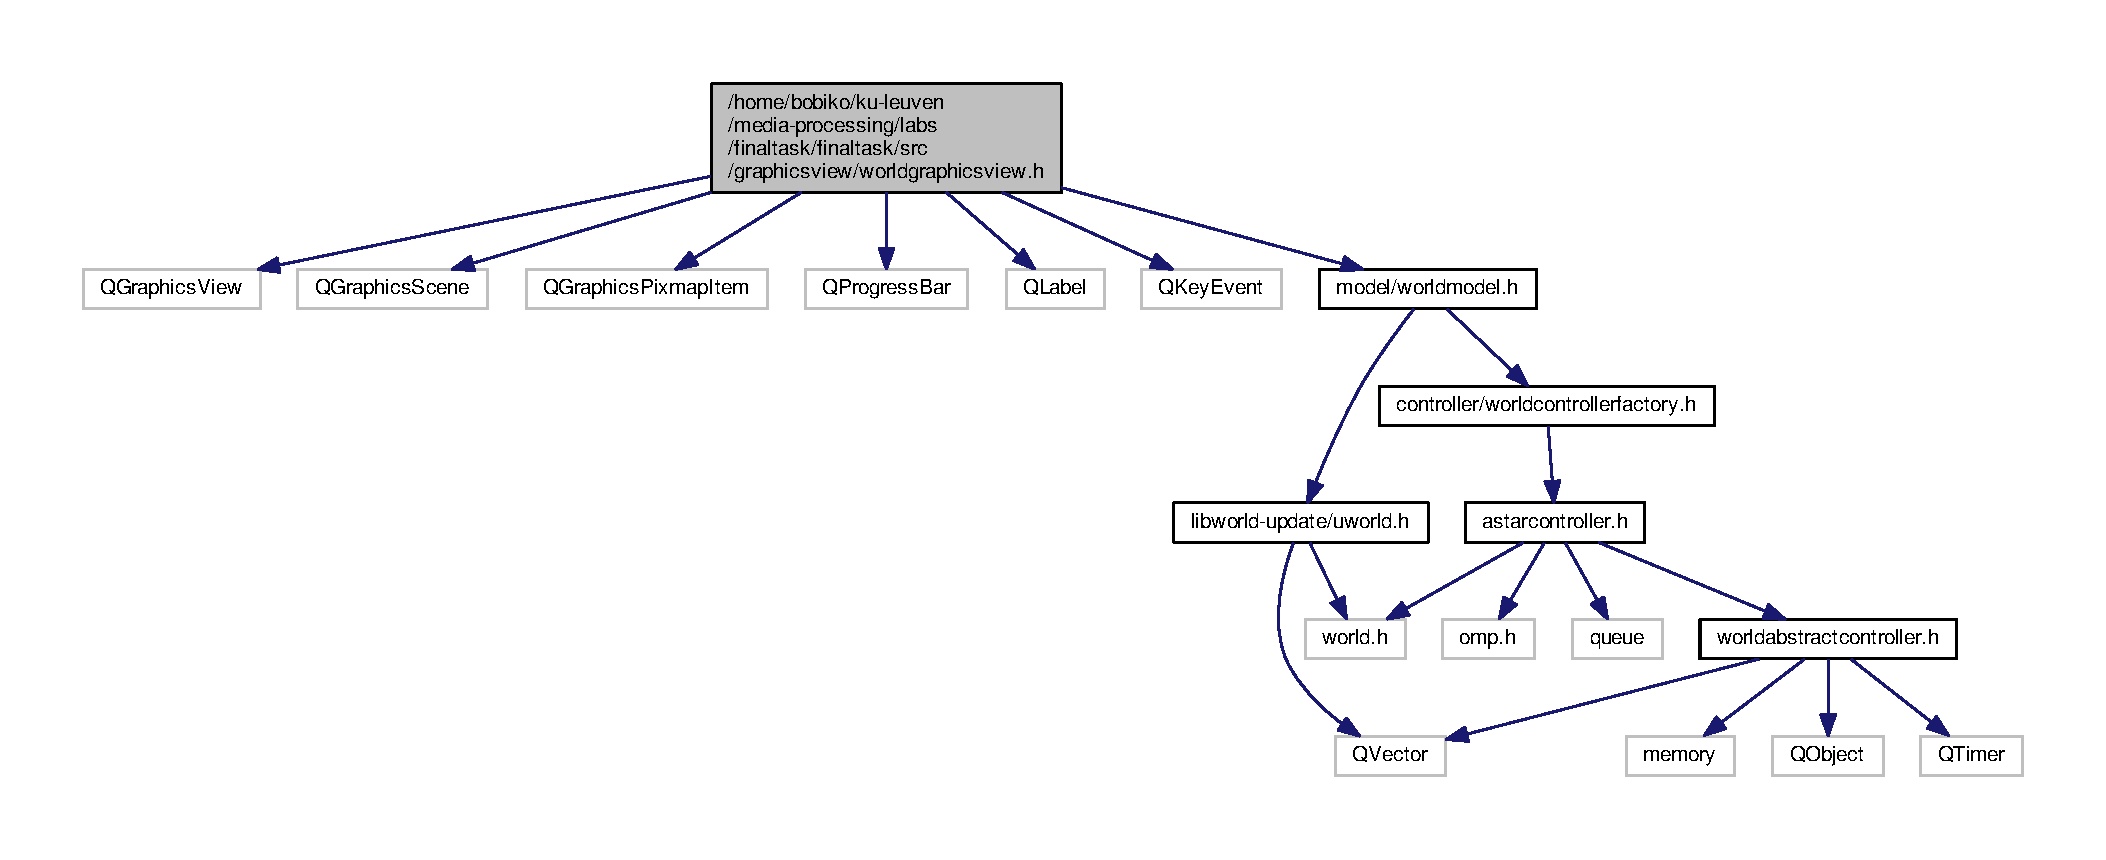
\includegraphics[width=350pt]{dd/d59/worldgraphicsview_8h__incl}
\end{center}
\end{figure}
This graph shows which files directly or indirectly include this file\+:
\nopagebreak
\begin{figure}[H]
\begin{center}
\leavevmode
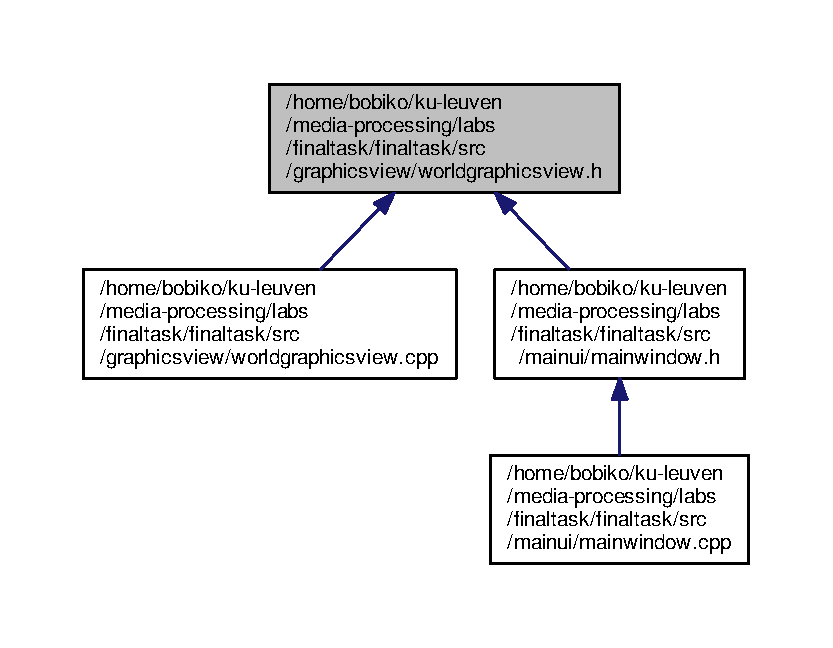
\includegraphics[width=350pt]{df/de5/worldgraphicsview_8h__dep__incl}
\end{center}
\end{figure}
\subsection*{Classes}
\begin{DoxyCompactItemize}
\item 
class \hyperlink{classWorldGraphicsView}{World\+Graphics\+View}
\begin{DoxyCompactList}\small\item\em Graphics view component class implementation. \end{DoxyCompactList}\end{DoxyCompactItemize}


\subsection{Detailed Description}
\hyperlink{classWorldGraphicsView}{World\+Graphics\+View} class declaration

\begin{DoxyVersion}{Version}
1.\+0
\end{DoxyVersion}
\begin{DoxyAuthor}{Author}
Vladimir Poliakov 

Brian Segers 

Kasper De Volder 
\end{DoxyAuthor}

\hypertarget{uworld_8cpp}{}\section{/home/bobiko/ku-\/leuven/media-\/processing/labs/finaltask/finaltask/src/libworld-\/update/uworld.cpp File Reference}
\label{uworld_8cpp}\index{/home/bobiko/ku-\/leuven/media-\/processing/labs/finaltask/finaltask/src/libworld-\/update/uworld.\+cpp@{/home/bobiko/ku-\/leuven/media-\/processing/labs/finaltask/finaltask/src/libworld-\/update/uworld.\+cpp}}
{\ttfamily \#include \char`\"{}uworld.\+h\char`\"{}}\\*
Include dependency graph for uworld.\+cpp\+:
\nopagebreak
\begin{figure}[H]
\begin{center}
\leavevmode
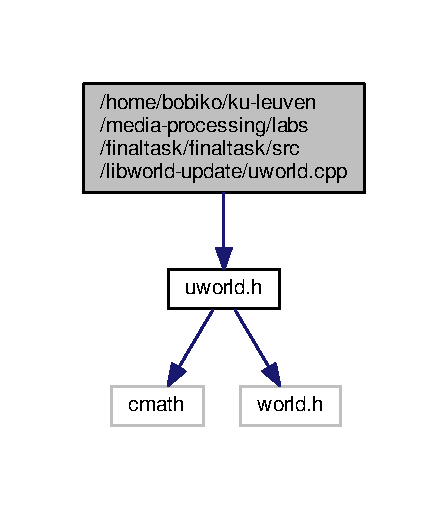
\includegraphics[width=215pt]{d0/d76/uworld_8cpp__incl}
\end{center}
\end{figure}


\subsection{Detailed Description}
libworld-\/update classes definition

\begin{DoxyVersion}{Version}
1.\+0
\end{DoxyVersion}
\begin{DoxyAuthor}{Author}
Vladimir Poliakov 

Brian Segers 

Kasper De Volder 
\end{DoxyAuthor}

\hypertarget{uworld_8h}{}\section{/home/bobiko/ku-\/leuven/media-\/processing/labs/finaltask/finaltask/src/libworld-\/update/uworld.h File Reference}
\label{uworld_8h}\index{/home/bobiko/ku-\/leuven/media-\/processing/labs/finaltask/finaltask/src/libworld-\/update/uworld.\+h@{/home/bobiko/ku-\/leuven/media-\/processing/labs/finaltask/finaltask/src/libworld-\/update/uworld.\+h}}
{\ttfamily \#include $<$Q\+Vector$>$}\\*
{\ttfamily \#include \char`\"{}world.\+h\char`\"{}}\\*
Include dependency graph for uworld.\+h\+:
\nopagebreak
\begin{figure}[H]
\begin{center}
\leavevmode
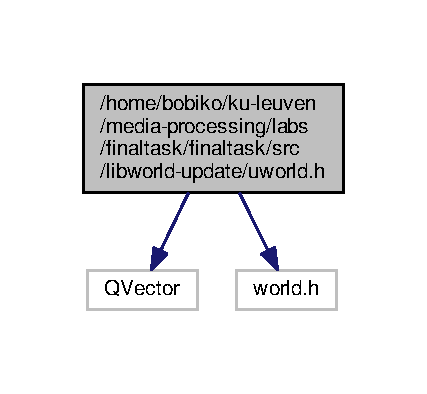
\includegraphics[width=205pt]{db/d9d/uworld_8h__incl}
\end{center}
\end{figure}
This graph shows which files directly or indirectly include this file\+:
\nopagebreak
\begin{figure}[H]
\begin{center}
\leavevmode
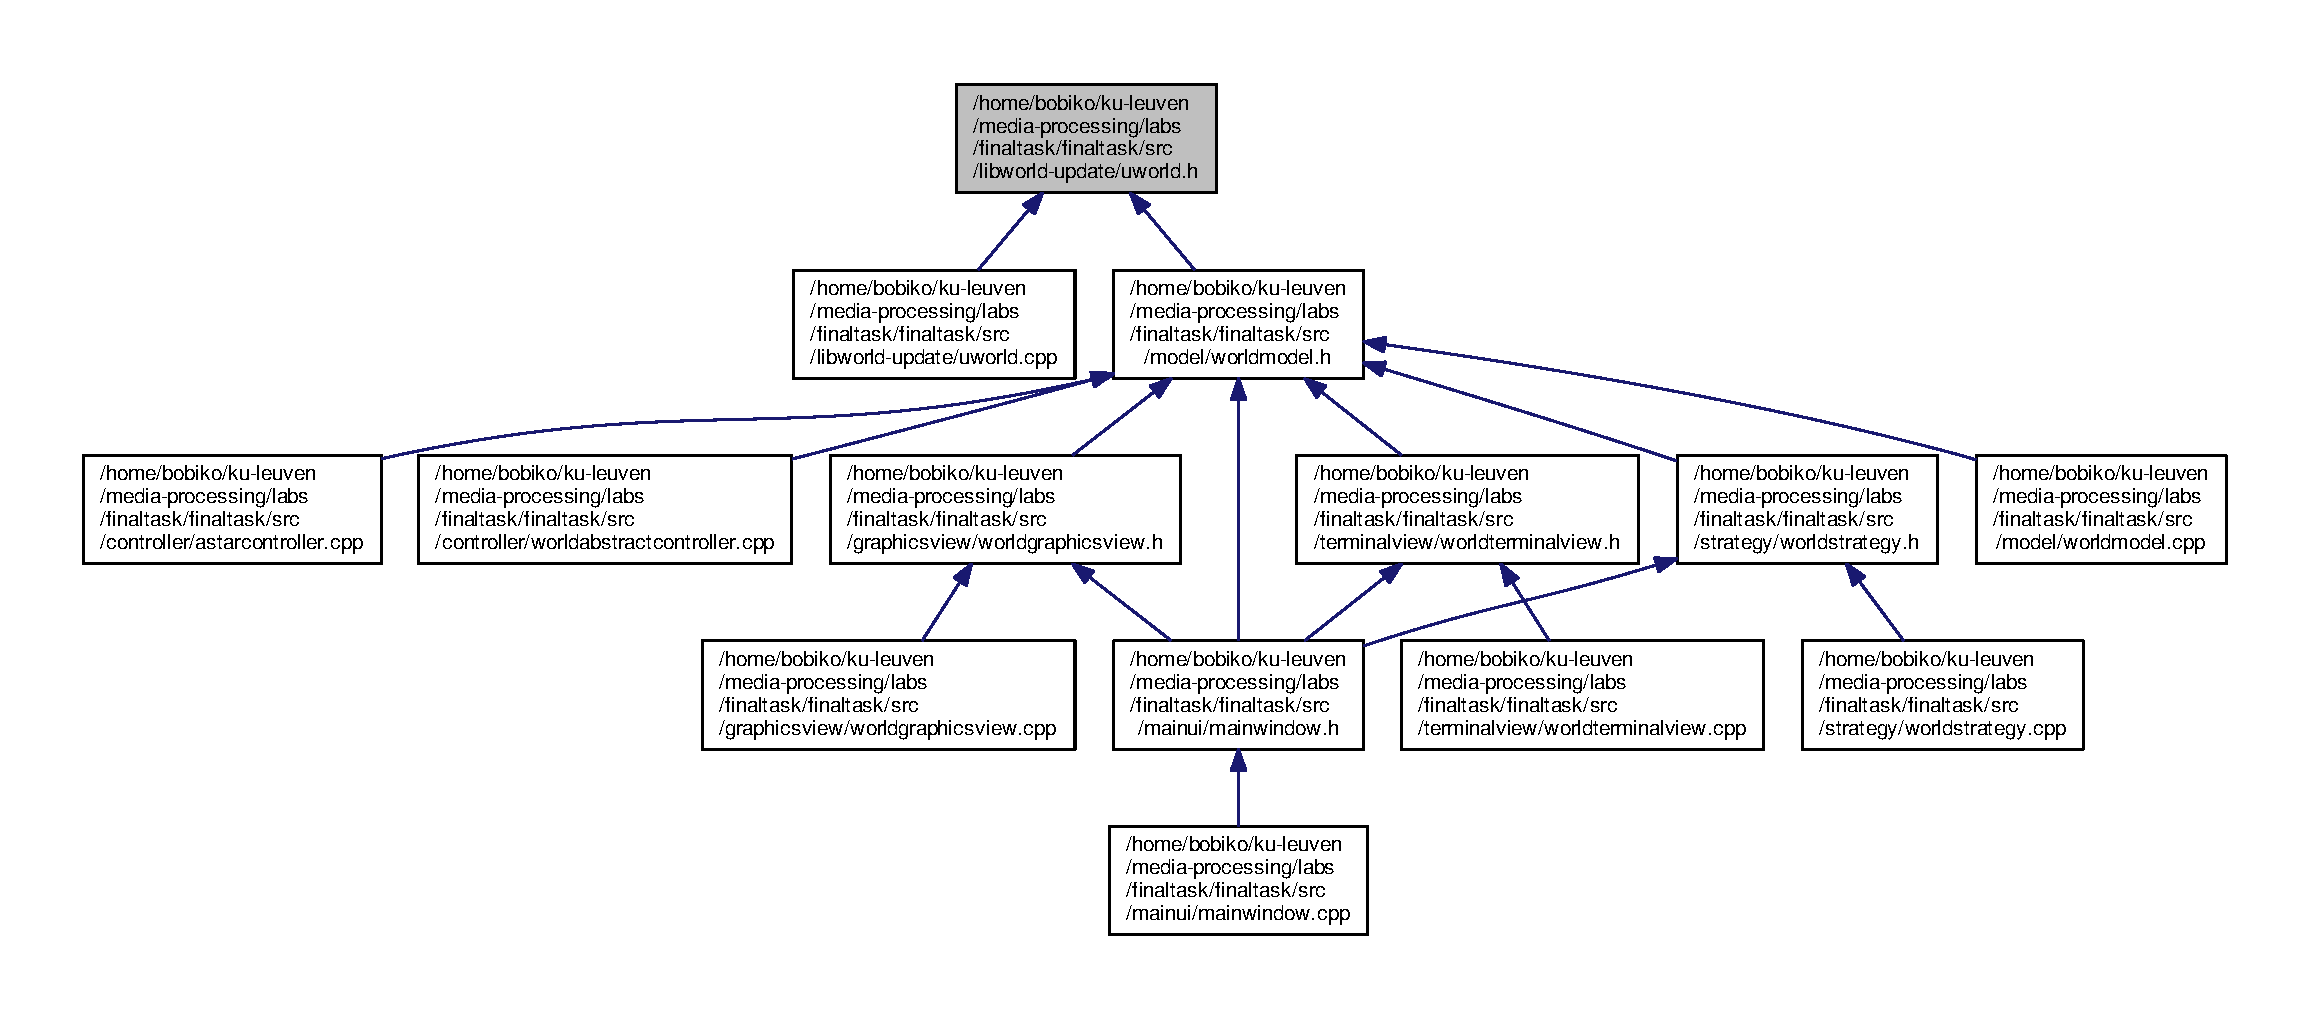
\includegraphics[width=350pt]{d7/ded/uworld_8h__dep__incl}
\end{center}
\end{figure}
\subsection*{Classes}
\begin{DoxyCompactItemize}
\item 
class \hyperlink{classUHealthPack}{U\+Health\+Pack}
\begin{DoxyCompactList}\small\item\em Updated health pack class. \end{DoxyCompactList}\item 
class \hyperlink{classUEnemy}{U\+Enemy}
\begin{DoxyCompactList}\small\item\em Updated enemy class. \end{DoxyCompactList}\item 
class \hyperlink{classUPEnemy}{U\+P\+Enemy}
\begin{DoxyCompactList}\small\item\em Updated poisoned enemy class. \end{DoxyCompactList}\item 
class \hyperlink{classUProtagonist}{U\+Protagonist}
\begin{DoxyCompactList}\small\item\em Updated protagonist class. \end{DoxyCompactList}\item 
class \hyperlink{classUWorld}{U\+World}
\begin{DoxyCompactList}\small\item\em Updated world class. \end{DoxyCompactList}\end{DoxyCompactItemize}


\subsection{Detailed Description}
libworld-\/update classes declaration

\begin{DoxyVersion}{Version}
1.\+0
\end{DoxyVersion}
\begin{DoxyAuthor}{Author}
Vladimir Poliakov 

Brian Segers 

Kasper De Volder 
\end{DoxyAuthor}

\hypertarget{mainwindow_8cpp}{}\section{/home/bobiko/ku-\/leuven/media-\/processing/labs/finaltask/finaltask/src/mainui/mainwindow.cpp File Reference}
\label{mainwindow_8cpp}\index{/home/bobiko/ku-\/leuven/media-\/processing/labs/finaltask/finaltask/src/mainui/mainwindow.\+cpp@{/home/bobiko/ku-\/leuven/media-\/processing/labs/finaltask/finaltask/src/mainui/mainwindow.\+cpp}}
{\ttfamily \#include \char`\"{}mainwindow.\+h\char`\"{}}\\*
{\ttfamily \#include \char`\"{}ui\+\_\+mainwindow.\+h\char`\"{}}\\*
Include dependency graph for mainwindow.\+cpp\+:
\nopagebreak
\begin{figure}[H]
\begin{center}
\leavevmode
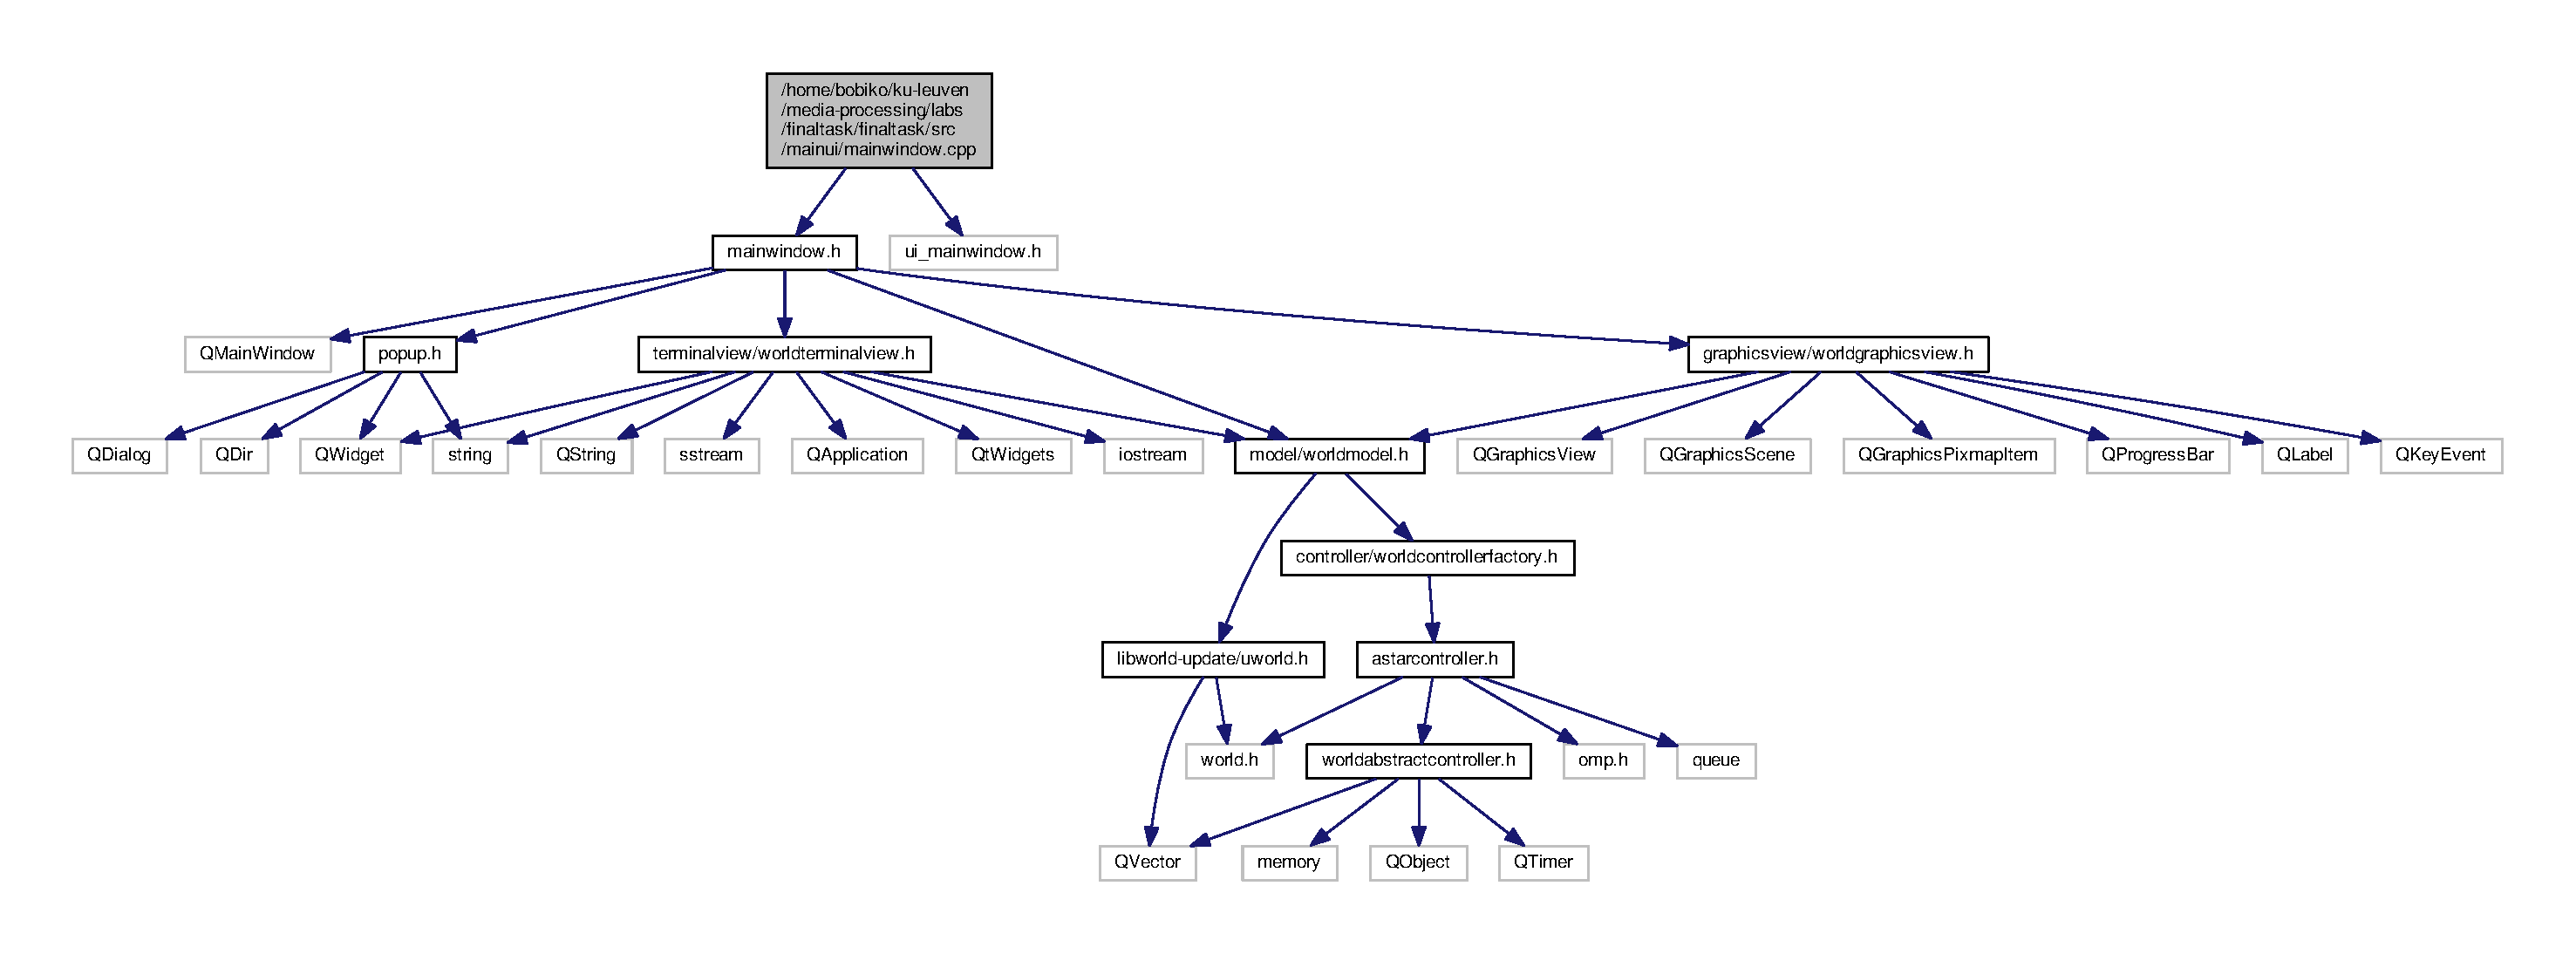
\includegraphics[width=350pt]{d1/dd5/mainwindow_8cpp__incl}
\end{center}
\end{figure}


\subsection{Detailed Description}
\hyperlink{classMainWindow}{Main\+Window} class definition

\begin{DoxyVersion}{Version}
1.\+0
\end{DoxyVersion}
\begin{DoxyAuthor}{Author}
Vladimir Poliakov 

Brian Segers 

Kasper De Volder 
\end{DoxyAuthor}

\hypertarget{mainwindow_8h}{}\section{/home/bobiko/ku-\/leuven/media-\/processing/labs/finaltask/finaltask/src/mainui/mainwindow.h File Reference}
\label{mainwindow_8h}\index{/home/bobiko/ku-\/leuven/media-\/processing/labs/finaltask/finaltask/src/mainui/mainwindow.\+h@{/home/bobiko/ku-\/leuven/media-\/processing/labs/finaltask/finaltask/src/mainui/mainwindow.\+h}}
{\ttfamily \#include $<$Q\+Main\+Window$>$}\\*
{\ttfamily \#include \char`\"{}terminalview/worldterminalview.\+h\char`\"{}}\\*
{\ttfamily \#include \char`\"{}graphicsview/worldgraphicsview.\+h\char`\"{}}\\*
{\ttfamily \#include \char`\"{}model/worldmodel.\+h\char`\"{}}\\*
{\ttfamily \#include \char`\"{}popup.\+h\char`\"{}}\\*
Include dependency graph for mainwindow.\+h\+:
\nopagebreak
\begin{figure}[H]
\begin{center}
\leavevmode
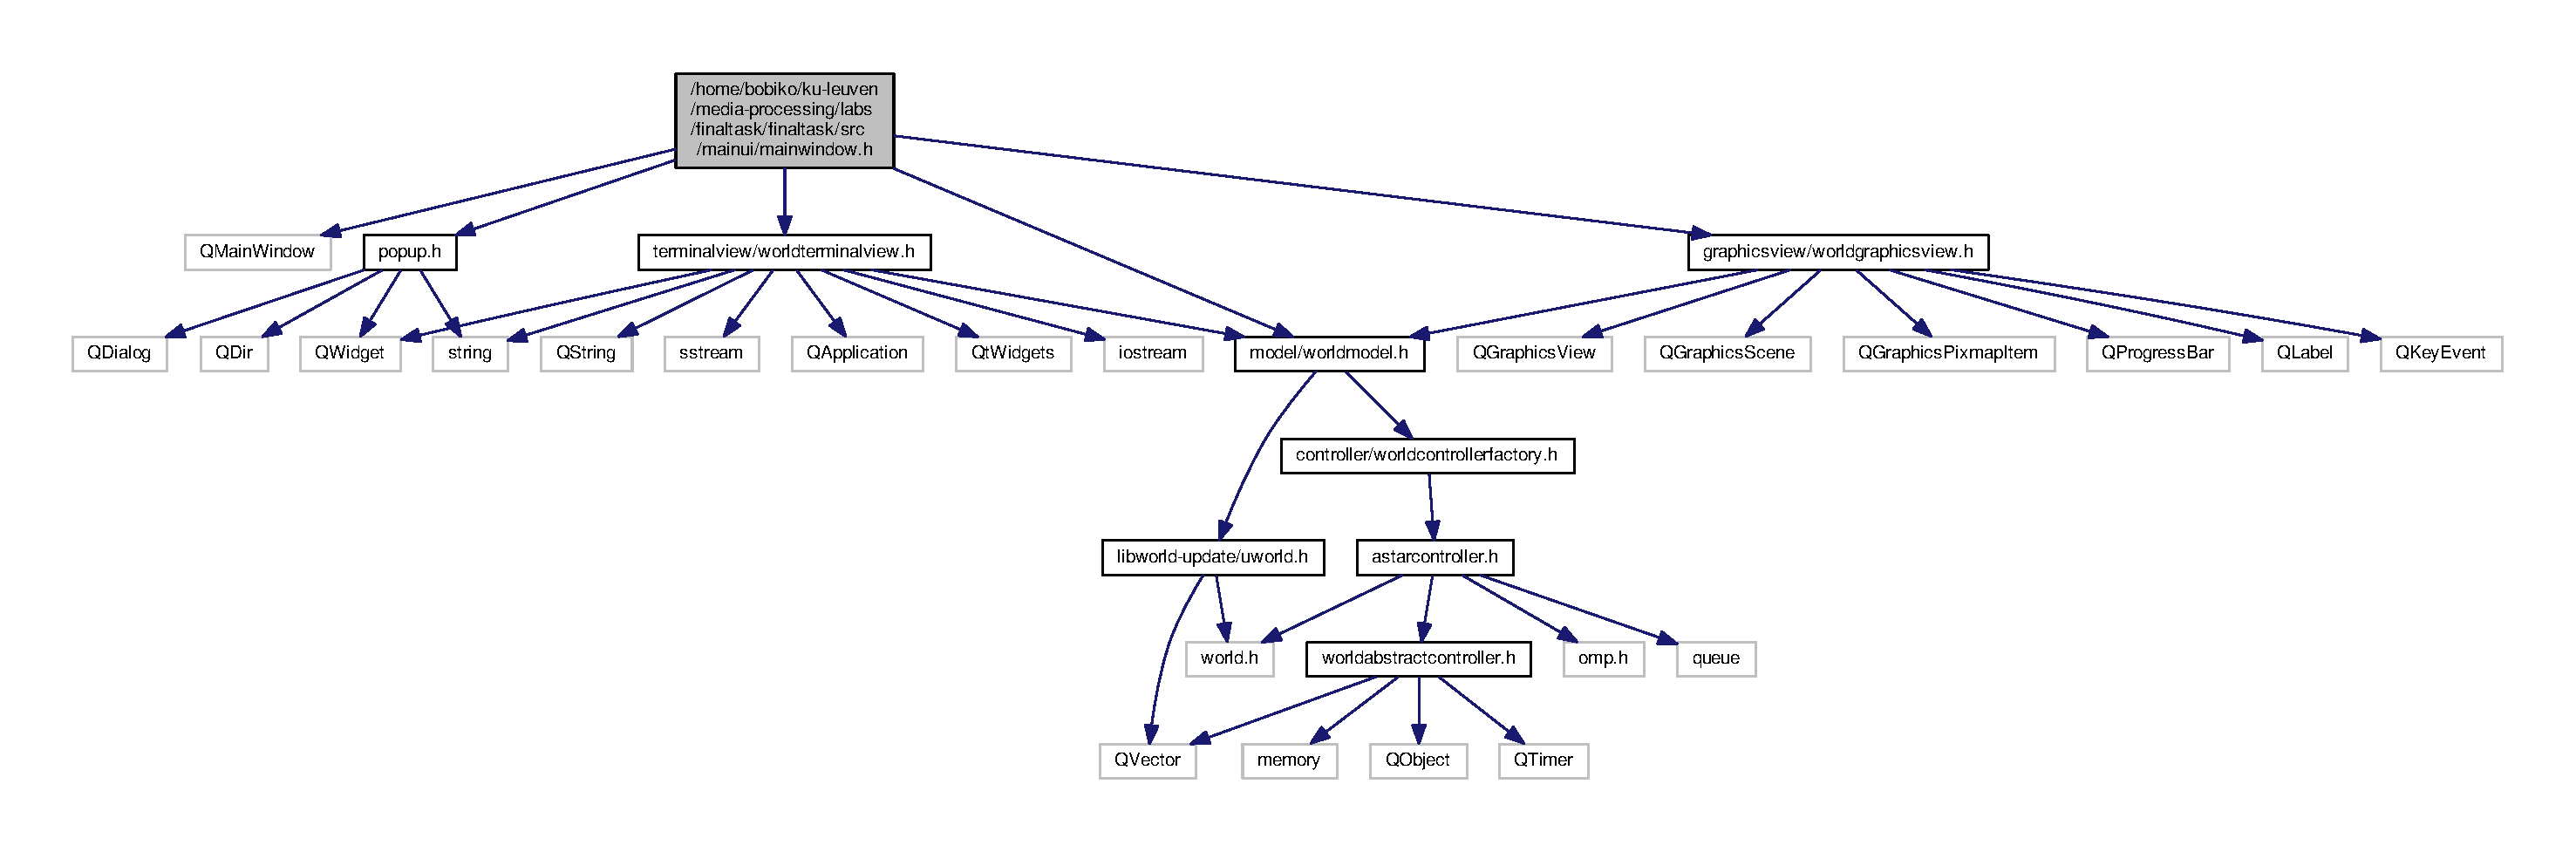
\includegraphics[width=350pt]{d2/d32/mainwindow_8h__incl}
\end{center}
\end{figure}
This graph shows which files directly or indirectly include this file\+:
\nopagebreak
\begin{figure}[H]
\begin{center}
\leavevmode
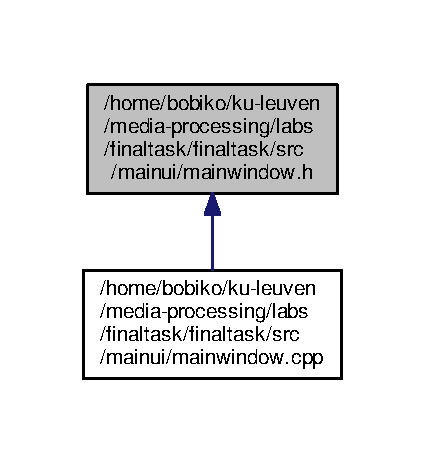
\includegraphics[width=204pt]{dc/d59/mainwindow_8h__dep__incl}
\end{center}
\end{figure}
\subsection*{Classes}
\begin{DoxyCompactItemize}
\item 
class \hyperlink{classMainWindow}{Main\+Window}
\begin{DoxyCompactList}\small\item\em Main window of the application. \end{DoxyCompactList}\end{DoxyCompactItemize}


\subsection{Detailed Description}
\hyperlink{classMainWindow}{Main\+Window} class declaration

\begin{DoxyVersion}{Version}
1.\+0
\end{DoxyVersion}
\begin{DoxyAuthor}{Author}
Vladimir Poliakov 

Brian Segers 

Kasper De Volder 
\end{DoxyAuthor}

\hypertarget{popup_8cpp}{}\section{/home/bobiko/ku-\/leuven/media-\/processing/labs/finaltask/finaltask/src/mainui/popup.cpp File Reference}
\label{popup_8cpp}\index{/home/bobiko/ku-\/leuven/media-\/processing/labs/finaltask/finaltask/src/mainui/popup.\+cpp@{/home/bobiko/ku-\/leuven/media-\/processing/labs/finaltask/finaltask/src/mainui/popup.\+cpp}}
{\ttfamily \#include \char`\"{}popup.\+h\char`\"{}}\\*
{\ttfamily \#include \char`\"{}ui\+\_\+popup.\+h\char`\"{}}\\*
Include dependency graph for popup.\+cpp\+:
\nopagebreak
\begin{figure}[H]
\begin{center}
\leavevmode
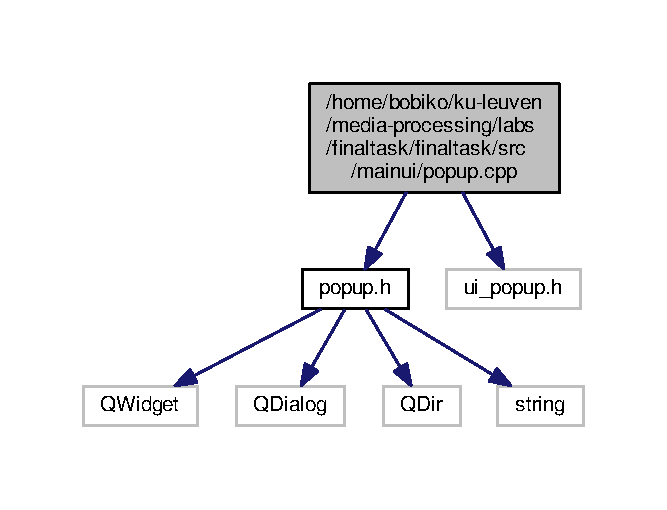
\includegraphics[width=320pt]{dc/d01/popup_8cpp__incl}
\end{center}
\end{figure}


\subsection{Detailed Description}
Startup dialog class definition

\begin{DoxyVersion}{Version}
1.\+0
\end{DoxyVersion}
\begin{DoxyAuthor}{Author}
Vladimir Poliakov 

Brian Segers 

Kasper De Volder 
\end{DoxyAuthor}

\hypertarget{popup_8h}{}\section{/home/bobiko/ku-\/leuven/media-\/processing/labs/finaltask/finaltask/src/mainui/popup.h File Reference}
\label{popup_8h}\index{/home/bobiko/ku-\/leuven/media-\/processing/labs/finaltask/finaltask/src/mainui/popup.\+h@{/home/bobiko/ku-\/leuven/media-\/processing/labs/finaltask/finaltask/src/mainui/popup.\+h}}
{\ttfamily \#include $<$Q\+Widget$>$}\\*
{\ttfamily \#include $<$Q\+Dialog$>$}\\*
{\ttfamily \#include $<$Q\+Dir$>$}\\*
{\ttfamily \#include $<$string$>$}\\*
Include dependency graph for popup.\+h\+:\nopagebreak
\begin{figure}[H]
\begin{center}
\leavevmode
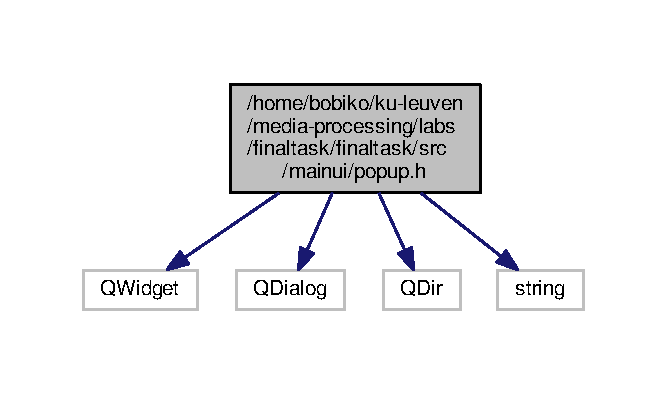
\includegraphics[width=320pt]{db/d6d/popup_8h__incl}
\end{center}
\end{figure}
This graph shows which files directly or indirectly include this file\+:\nopagebreak
\begin{figure}[H]
\begin{center}
\leavevmode
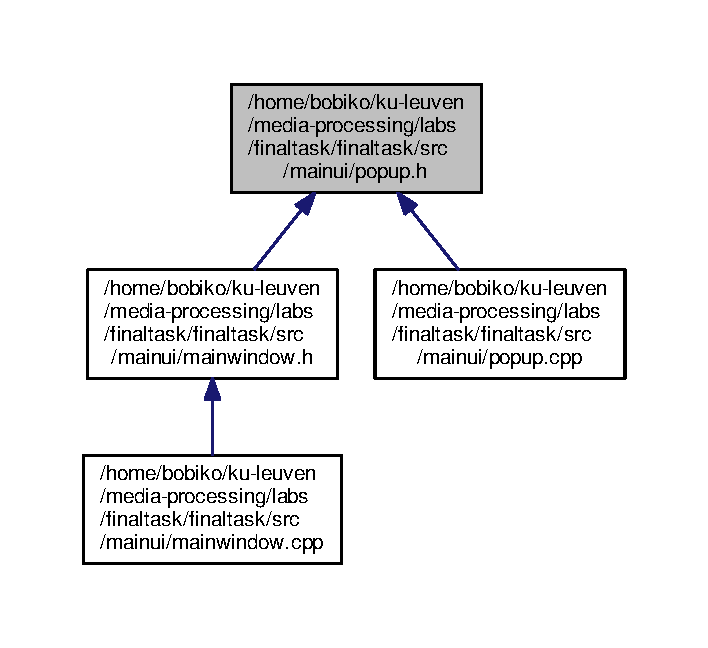
\includegraphics[width=340pt]{d3/db9/popup_8h__dep__incl}
\end{center}
\end{figure}
\subsection*{Classes}
\begin{DoxyCompactItemize}
\item 
struct \hyperlink{structValues}{Values}
\begin{DoxyCompactList}\small\item\em Current values of \hyperlink{classPopup}{Popup} controls. \end{DoxyCompactList}\item 
class \hyperlink{classPopup}{Popup}
\begin{DoxyCompactList}\small\item\em Stratup dialog class. \end{DoxyCompactList}\end{DoxyCompactItemize}


\subsection{Detailed Description}
Startup dialog class declaration

\begin{DoxyVersion}{Version}
1.\+0
\end{DoxyVersion}
\begin{DoxyAuthor}{Author}
Vladimir Poliakov 

Brian Segers 

Kasper De Volder 
\end{DoxyAuthor}

\hypertarget{worldmodel_8cpp}{}\section{/home/bobiko/ku-\/leuven/media-\/processing/labs/finaltask/finaltask/src/model/worldmodel.cpp File Reference}
\label{worldmodel_8cpp}\index{/home/bobiko/ku-\/leuven/media-\/processing/labs/finaltask/finaltask/src/model/worldmodel.\+cpp@{/home/bobiko/ku-\/leuven/media-\/processing/labs/finaltask/finaltask/src/model/worldmodel.\+cpp}}
{\ttfamily \#include \char`\"{}worldmodel.\+h\char`\"{}}\\*
Include dependency graph for worldmodel.\+cpp\+:\nopagebreak
\begin{figure}[H]
\begin{center}
\leavevmode
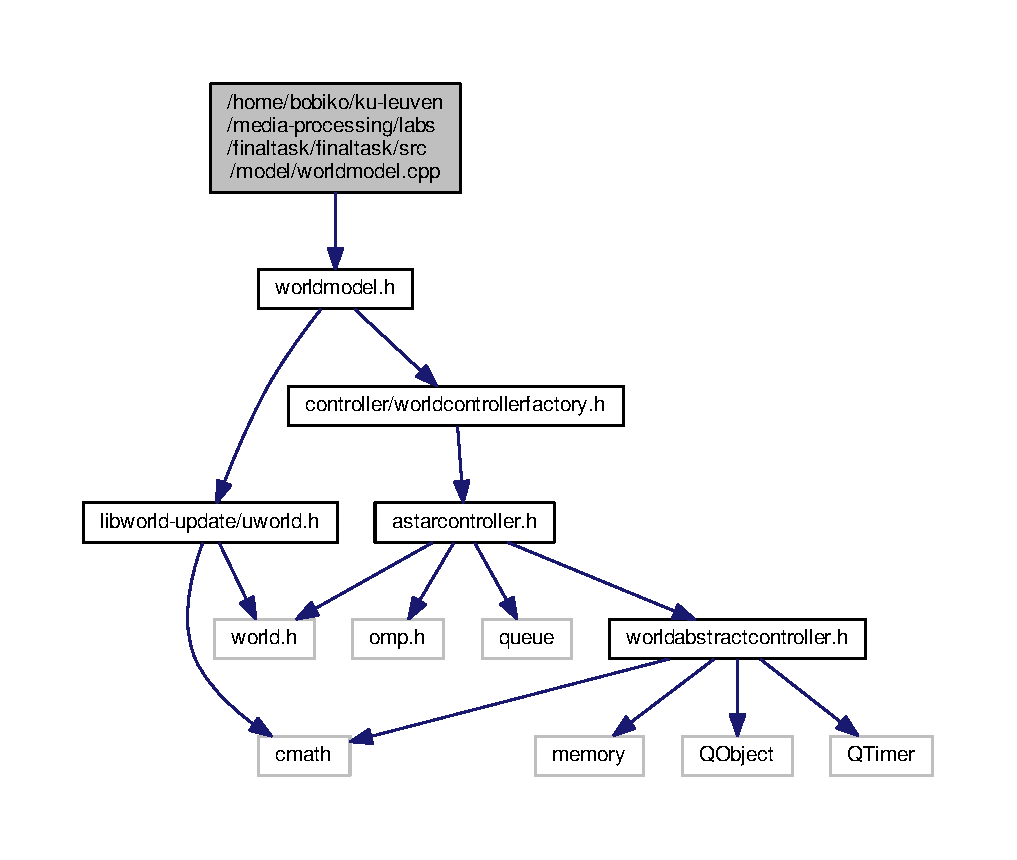
\includegraphics[width=350pt]{df/d31/worldmodel_8cpp__incl}
\end{center}
\end{figure}


\subsection{Detailed Description}
\hyperlink{classWorldModel}{World\+Model} class definition

\begin{DoxyVersion}{Version}
1.\+0
\end{DoxyVersion}
\begin{DoxyAuthor}{Author}
Vladimir Poliakov 

Brian Segers 

Kasper De Volder 
\end{DoxyAuthor}

\hypertarget{worldmodel_8h}{}\section{/home/bobiko/ku-\/leuven/media-\/processing/labs/finaltask/finaltask/src/model/worldmodel.h File Reference}
\label{worldmodel_8h}\index{/home/bobiko/ku-\/leuven/media-\/processing/labs/finaltask/finaltask/src/model/worldmodel.\+h@{/home/bobiko/ku-\/leuven/media-\/processing/labs/finaltask/finaltask/src/model/worldmodel.\+h}}
{\ttfamily \#include \char`\"{}libworld-\/update/uworld.\+h\char`\"{}}\\*
{\ttfamily \#include \char`\"{}controller/worldcontrollerfactory.\+h\char`\"{}}\\*
Include dependency graph for worldmodel.\+h\+:
\nopagebreak
\begin{figure}[H]
\begin{center}
\leavevmode
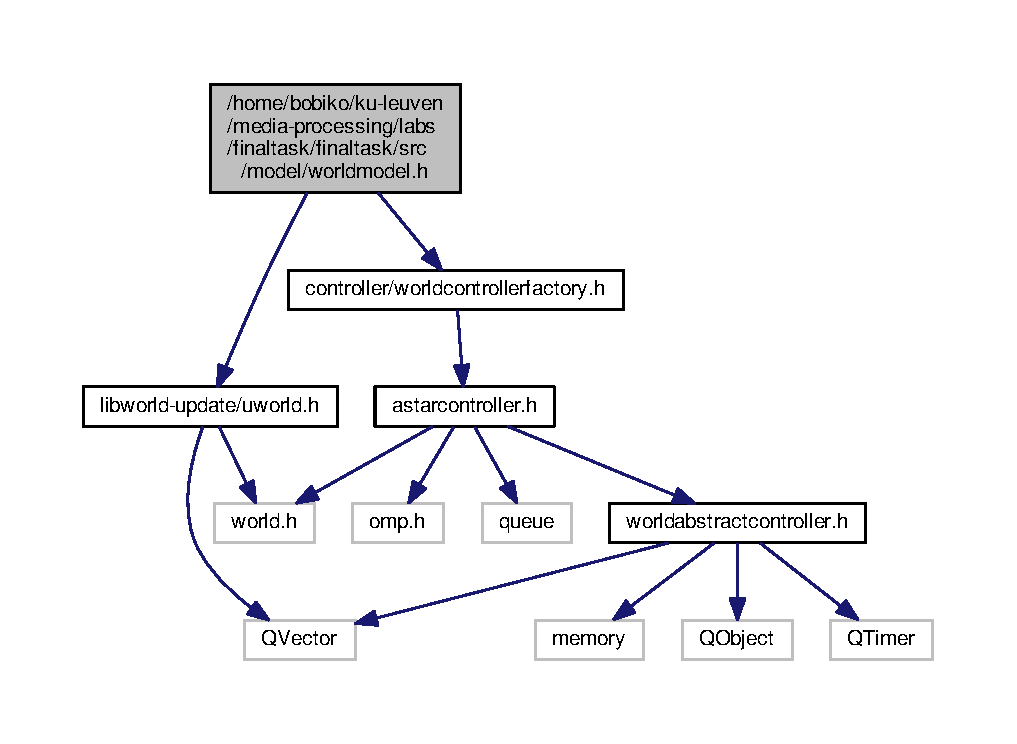
\includegraphics[width=350pt]{d8/d5b/worldmodel_8h__incl}
\end{center}
\end{figure}
This graph shows which files directly or indirectly include this file\+:
\nopagebreak
\begin{figure}[H]
\begin{center}
\leavevmode
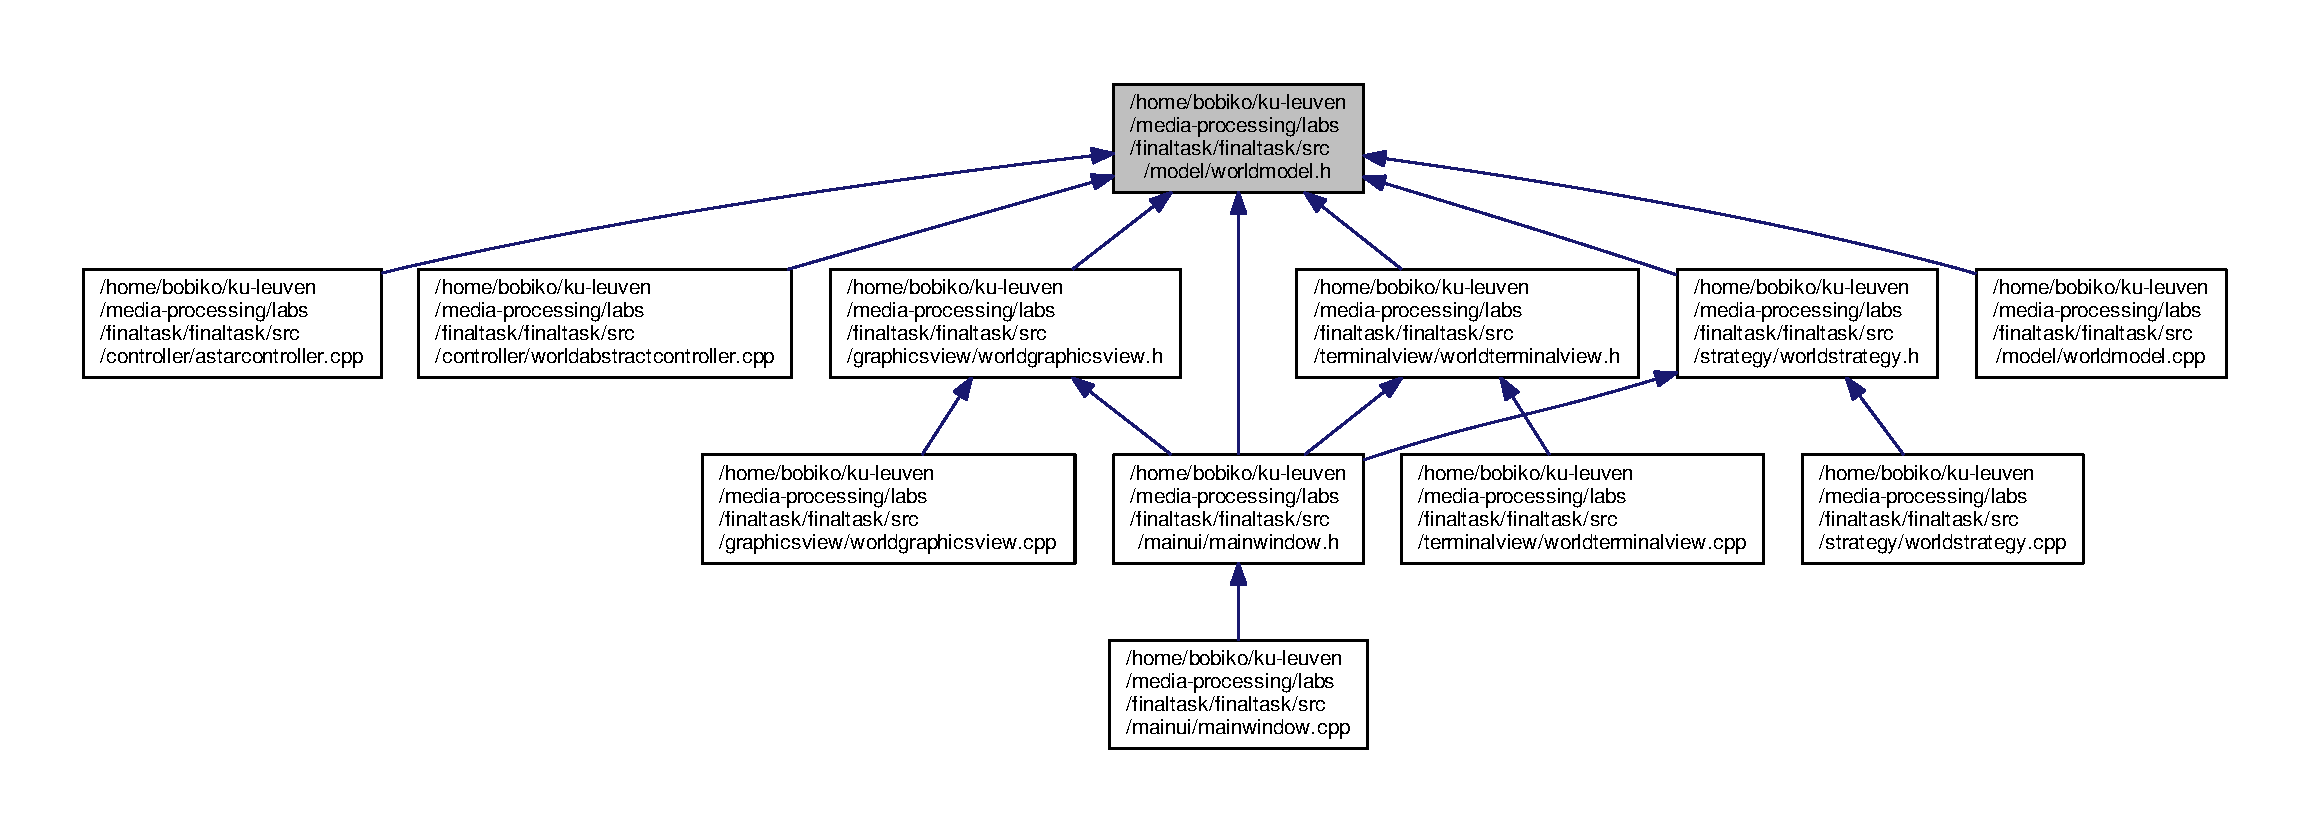
\includegraphics[width=350pt]{d2/d38/worldmodel_8h__dep__incl}
\end{center}
\end{figure}
\subsection*{Classes}
\begin{DoxyCompactItemize}
\item 
class \hyperlink{classWorldModel}{World\+Model}
\begin{DoxyCompactList}\small\item\em Model component implementation. \end{DoxyCompactList}\end{DoxyCompactItemize}


\subsection{Detailed Description}
\hyperlink{classWorldModel}{World\+Model} class declaration

\begin{DoxyVersion}{Version}
1.\+0
\end{DoxyVersion}
\begin{DoxyAuthor}{Author}
Vladimir Poliakov 

Brian Segers 

Kasper De Volder 
\end{DoxyAuthor}

\hypertarget{worldterminalview_8cpp}{}\section{/home/bobiko/ku-\/leuven/media-\/processing/labs/finaltask/finaltask/src/terminalview/worldterminalview.cpp File Reference}
\label{worldterminalview_8cpp}\index{/home/bobiko/ku-\/leuven/media-\/processing/labs/finaltask/finaltask/src/terminalview/worldterminalview.\+cpp@{/home/bobiko/ku-\/leuven/media-\/processing/labs/finaltask/finaltask/src/terminalview/worldterminalview.\+cpp}}
{\ttfamily \#include \char`\"{}worldterminalview.\+h\char`\"{}}\\*
Include dependency graph for worldterminalview.\+cpp\+:
\nopagebreak
\begin{figure}[H]
\begin{center}
\leavevmode
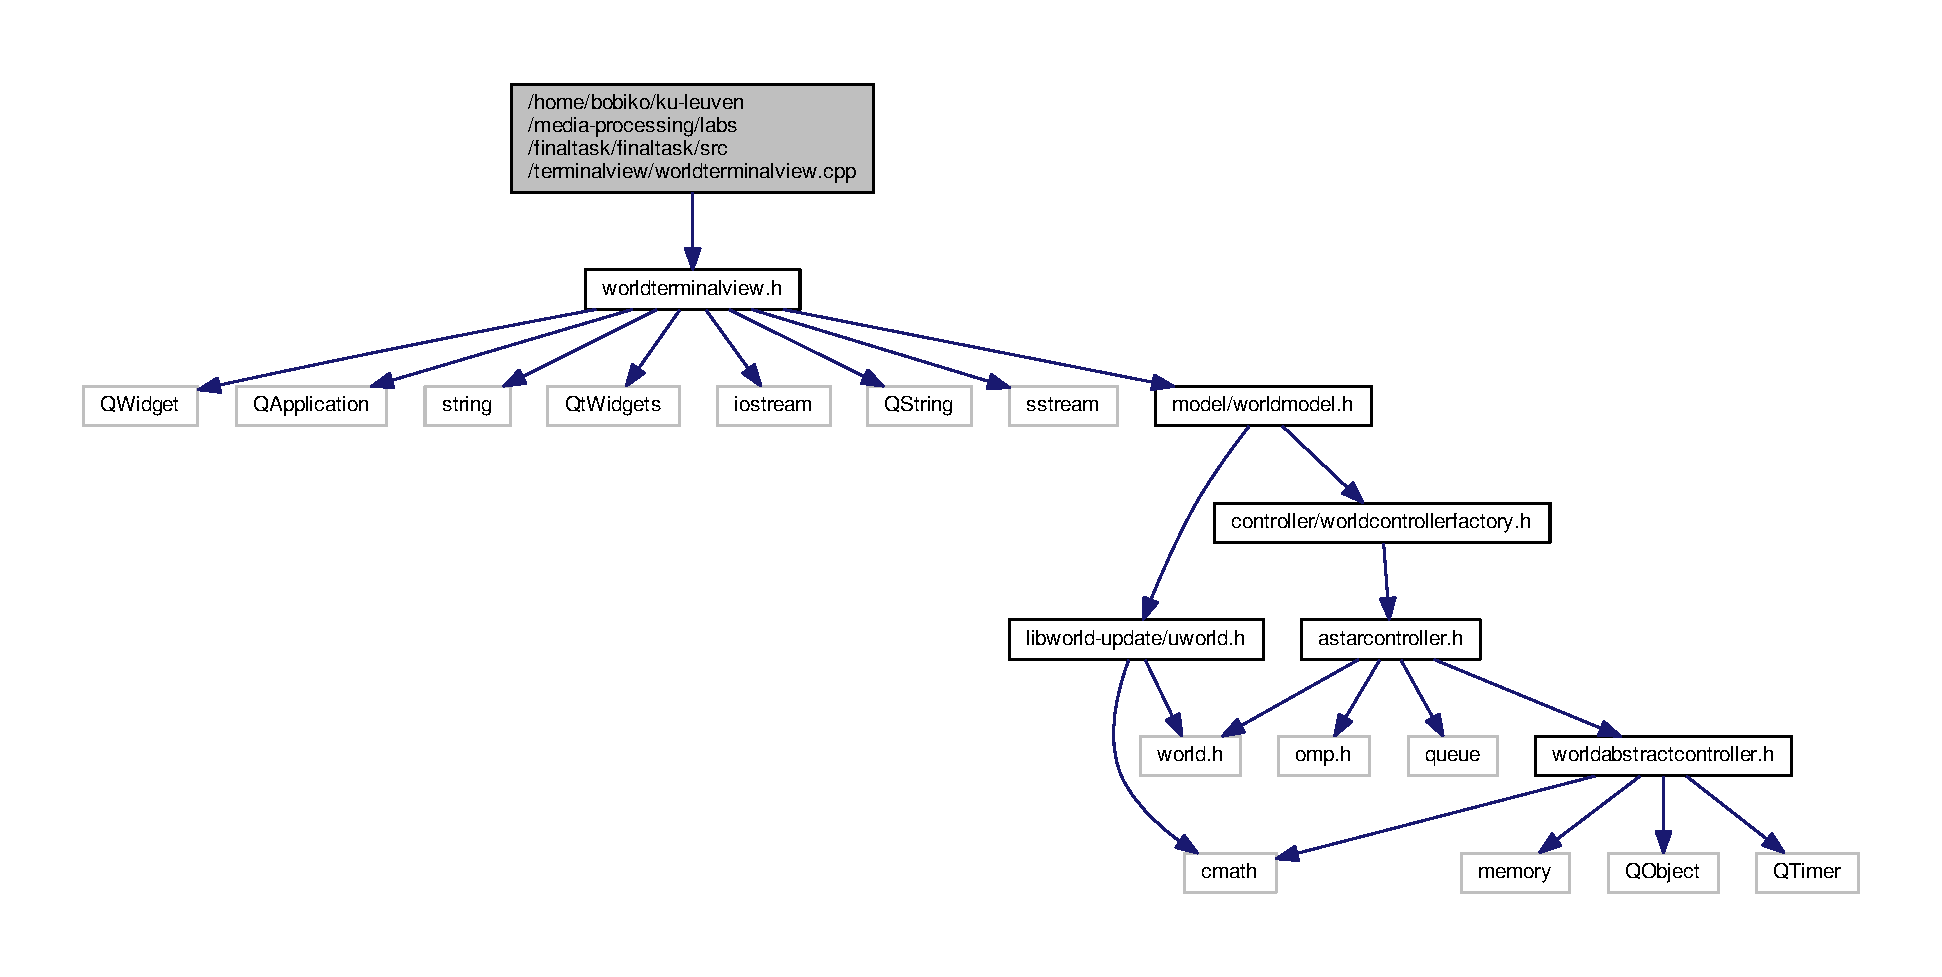
\includegraphics[width=350pt]{dc/d71/worldterminalview_8cpp__incl}
\end{center}
\end{figure}


\subsection{Detailed Description}
\hyperlink{classWorldTerminalView}{World\+Terminal\+View} class definition

\begin{DoxyVersion}{Version}
1.\+0
\end{DoxyVersion}
\begin{DoxyAuthor}{Author}
Vladimir Poliakov 

Brian Segers 

Kasper De Volder 
\end{DoxyAuthor}

\hypertarget{worldterminalview_8h}{}\section{/home/bobiko/ku-\/leuven/media-\/processing/labs/finaltask/finaltask/src/terminalview/worldterminalview.h File Reference}
\label{worldterminalview_8h}\index{/home/bobiko/ku-\/leuven/media-\/processing/labs/finaltask/finaltask/src/terminalview/worldterminalview.\+h@{/home/bobiko/ku-\/leuven/media-\/processing/labs/finaltask/finaltask/src/terminalview/worldterminalview.\+h}}
{\ttfamily \#include $<$Q\+Widget$>$}\\*
{\ttfamily \#include $<$Q\+Application$>$}\\*
{\ttfamily \#include $<$string$>$}\\*
{\ttfamily \#include $<$Qt\+Widgets$>$}\\*
{\ttfamily \#include $<$iostream$>$}\\*
{\ttfamily \#include $<$Q\+String$>$}\\*
{\ttfamily \#include $<$sstream$>$}\\*
{\ttfamily \#include \char`\"{}model/worldmodel.\+h\char`\"{}}\\*
Include dependency graph for worldterminalview.\+h\+:
\nopagebreak
\begin{figure}[H]
\begin{center}
\leavevmode
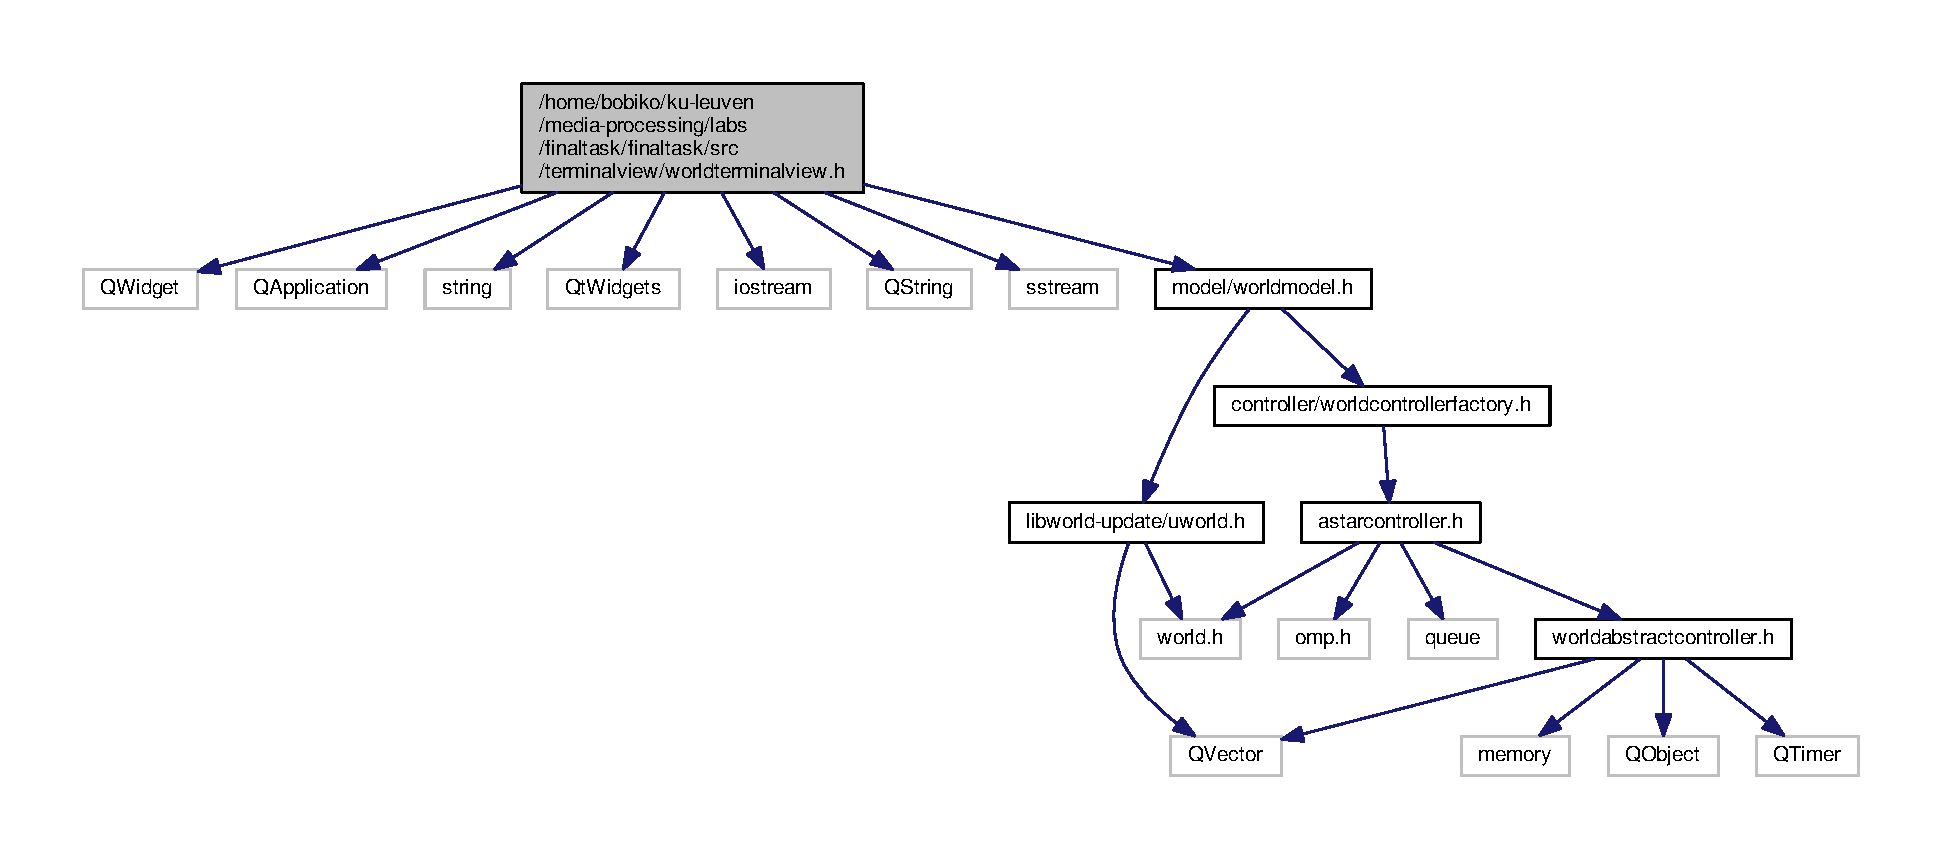
\includegraphics[width=350pt]{dd/d49/worldterminalview_8h__incl}
\end{center}
\end{figure}
This graph shows which files directly or indirectly include this file\+:
\nopagebreak
\begin{figure}[H]
\begin{center}
\leavevmode
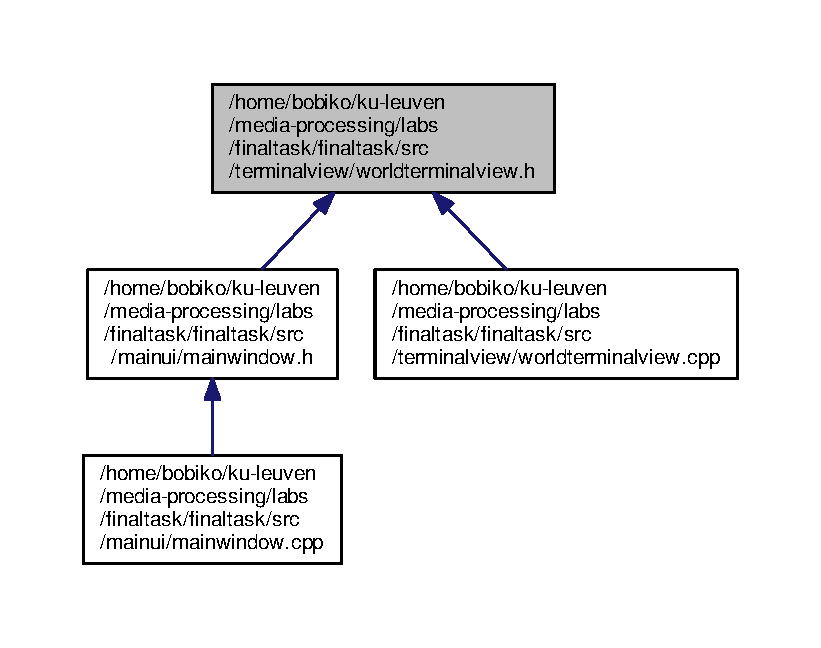
\includegraphics[width=350pt]{db/d4a/worldterminalview_8h__dep__incl}
\end{center}
\end{figure}
\subsection*{Classes}
\begin{DoxyCompactItemize}
\item 
class \hyperlink{classWorldTerminalView}{World\+Terminal\+View}
\begin{DoxyCompactList}\small\item\em The \hyperlink{classWorldTerminalView}{World\+Terminal\+View} class. \end{DoxyCompactList}\end{DoxyCompactItemize}


\subsection{Detailed Description}
\hyperlink{classWorldTerminalView}{World\+Terminal\+View} class declaration

\begin{DoxyVersion}{Version}
1.\+0
\end{DoxyVersion}
\begin{DoxyAuthor}{Author}
Vladimir Poliakov 

Brian Segers 

Kasper De Volder 
\end{DoxyAuthor}

%--- End generated contents ---

% Index
\backmatter
\newpage
\phantomsection
\clearemptydoublepage
\addcontentsline{toc}{chapter}{Index}
\printindex

\end{document}
